% Arquivo principal para trabalhos acadêmicos da UDESC - Joinville

% abnTeX2: Modelo de Trabalho Academico em conformidade com 
% ABNT NBR 14724:2011: Informacao e documentacao - Trabalhos academicos -
% Apresentacao

% Edited by: Eduardo H. Couto
% e-mail: ehcouto@hotmail.com
% ------------------------------------------------------------------------
% ------------------------------------------------------------------------

\documentclass[
	12pt,				% tamanho da fonte
	openright,			% capítulos começam em pág ímpar (insere página vazia caso preciso)
	oneside,			% para impressão em verso e anverso. Oposto a oneside
	a4paper,			% tamanho do papel. 
	chapter=TITLE,		% títulos de capítulos convertidos em letras maiúsculas
	%section=TITLE,		% títulos de seções convertidos em letras maiúsculas
	%subsection=TITLE,	% títulos de subseções convertidos em letras maiúsculas
	%subsubsection=TITLE,% títulos de subsubseções convertidos em letras maiúsculas
	% -- opções do pacote babel --
	english,			% idioma adicional para hifenização
	brazil,				% o último idioma é o principal do documento
	]{./Data/udesc}

\usepackage{./Data/udescsty}
\usepackage{color,graphicx}
\usepackage[table,xcdraw]{xcolor}


% ---
% Informações de dados para CAPA e FOLHA DE ROSTO
% ---
\titulo{Agil It - Sistema Gerenciador de Ordens de Manutenção de
	Equipamento}
\autor{Julio Thomazelli Júnior, Lucas Matheus da Silva Gonçalves, Márcio Henrique Meier}
\local{Jaraguá do Sul}
\data{2019}
\fulldata{09 de Junho de 2019}
\orientador{Prof. Tathiana Duarte do Amarante}
\instituicao{Serviço Nacional de Aprendizagem Industrial - SENAI}
\tipodoc{Dissertação}
\curso{Sistemas para Internet}
\area{Gerenciamento de Ordens de Manutenção}
\preambulo{Projeto Integrador de Desenvolvimento de Software para a empresa DUAS RODAS}
% ---

% ----
% Início do documento
% ----
\begin{document}
% ----------------------------------------------------------
% ELEMENTOS PRÉ-TEXTUAIS
% ----------------------------------------------------------
% Retira espaço extra obsoleto entre as frases.
\frenchspacing 

% \pretextual

% ---
% Capa
% ---
\imprimircapa
% ---

% ---
% Folha de rosto
% (o * indica que haverá a ficha bibliográfica)
% ---
\imprimirfolhaderosto*
% ---

% ---
% Inserir a ficha bibliografica
% ---

% Isto é um exemplo de Ficha Catalográfica, ou ``Dados internacionais de
% catalogação-na-publicação''. Você pode utilizar este modelo como referência. 
% Porém, provavelmente a biblioteca da sua universidade lhe fornecerá um PDF
% com a ficha catalográfica definitiva após a defesa do trabalho. Quando estiver
% com o documento, salve-o como PDF no diretório do seu projeto e substitua todo
% o conteúdo de implementação deste arquivo pelo comando abaixo:
%
% \begin{fichacatalografica}
%     \includepdf{fig_ficha_catalografica.pdf}
% \end{fichacatalografica}
%\begin{fichacatalografica}
%	\vspace*{\fill}					% Posição vertical
%	\hrule							% Linha horizontal
%	\begin{center}					% Minipage Centralizado
%	\begin{minipage}[c]{12.5cm}		% Largura
%	
%	\imprimirautor
%	
%	\hspace{0.5cm} \imprimirtitulo  / \imprimirautor. --
%	\imprimirlocal, \imprimirdata-
%	
%	
%	\hspace{0.5cm} \imprimirorientadorRotulo~\imprimirorientador\\
%	
%	\hspace{0.5cm}
%	\parbox[t]{\textwidth}{\imprimirtipotrabalho~--~\imprimirinstituicao,
%	\imprimirdata.}\\
%	
%	
%	\end{minipage}
%	\end{center}
%	\hrule
%\end{fichacatalografica}
% ---


% ---
% Inserir errata (Se necessário)
% ---
%\begin{errata}
%Elemento opcional da \citeonline[4.2.1.2]{NBR14724:2011}. Exemplo:
%
%\vspace{\onelineskip}
%
%FERRIGNO, C. R. A. \textbf{Tratamento de neoplasias ósseas apendiculares com
%reimplantação de enxerto ósseo autólogo autoclavado associado ao plasma
%rico em plaquetas}: estudo crítico na cirurgia de preservação de membro em
%cães. 2011. 128 f. Tese (Livre-Docência) - Faculdade de Medicina Veterinária e
%Zootecnia, Universidade de São Paulo, São Paulo, 2011.
%
%\begin{table}[htb]
%\center
%\footnotesize
%\begin{tabular}{|p{1.4cm}|p{1cm}|p{3cm}|p{3cm}|}
%  \hline
%   \textbf{Folha} & \textbf{Linha}  & \textbf{Onde se lê}  & \textbf{Leia-se}  \\
%    \hline
%    1 & 10 & auto-conclavo & autoconclavo\\
%   \hline
%\end{tabular}
%\end{table}
%
%\end{errata}
% ---

% ---
% Inserir folha de aprovação
% ---

% Isto é um exemplo de Folha de aprovação, elemento obrigatório da NBR
% 14724/2011 (seção 4.2.1.3). Você pode utilizar este modelo até a aprovação
% do trabalho. Após isso, substitua todo o conteúdo deste arquivo por uma
% imagem da página assinada pela banca com o comando abaixo:
%
% \includepdf{folhadeaprovacao_final.pdf}
%
% ---

% ---
% Dedicatória
% ---
% ---

% ---
% Agradecimentos
% ---
% ---

% ---
% Epígrafe
% ---
% ---

% ---
% RESUMOS
% ---


% resumo em português
\begin{resumo}
	Atualmente, o processo de ordens de manutenção da indústria Duas Rodas é realizado manualmente, fazendo com que a empresa consuma muito papel, prejudicando o meio ambiente e como consequência, acabam se perdendo com a quantidade de informações acumuladas. Sendo assim, o projeto tem como objetivo apresentar e transformar o antigo processo em um fluxo totalmente digital com a aplicação web para gerenciar as ordens e a aplicação mobile para executá-las.
	
	\vspace{\onelineskip}
	
	\noindent
	\textbf{Palavras-chaves}: Sistema, WEB, Mobile, Ordem de Manutenção, Digital.
\end{resumo}

% resumo em inglês
\begin{resumo}[Abstract]
	\begin{otherlanguage*}{english}
		Currently, the maintenance order process for the Duas Rodas industry is carried out manually, causing the company to consume a lot of paper, damaging the environment and, as a consequence, they end up being lost with the amount of accumulated information. Therefore, the project aims to present and transform the old process into a fully digital flow with a web application to manage orders and a mobile application to execute them.
		
		\vspace{\onelineskip}
		
		\noindent 
		\textbf{Key-words}: System, WEB, Mobile, Maintenance Order, Digital.
	\end{otherlanguage*}
\end{resumo}


% ---
% inserir lista de ilustrações
% ---
\pdfbookmark[0]{\listfigurename}{lof}
\listoffigures*
\cleardoublepage
% ---

% ---
% inserir lista de tabelas
% ---
%\pdfbookmark[0]{\listtablename}{lot}
%\listoftables*
%\cleardoublepage
% ---

% ---
% inserir lista de abreviaturas e siglas
% ---
\begin{siglas}
  \item[MVP]      Minimum Viable Product
  \item[API]      Application Programming Interface
  \item[ORM]      Object-Relational Mapping
  \item[OM]		  Ordem de Manutenção
  \item[ERP]      Software de gerenciamento de empresas
  \item[SAP]	  ERP alemão conhecido mundialmente
  \item[WEB]	  Internet
  \item[UC]		  Unidade Curricular
\end{siglas}
% ---


% ---
% inserir o sumario
% ---
\pdfbookmark[0]{\contentsname}{toc}
\tableofcontents*
\cleardoublepage
% ---

\textual
% ---

% ----------------------------------------------------------
% ELEMENTOS TEXTUAIS
% ----------------------------------------------------------
\chapter{Introdução ao Documento}

A empresa Duas Rodas possui sua sede em Jaraguá do Sul, Santa Catarina e tem como principal ramo a indústria de alimentos \footnote{\url{ https://www.duasrodas.com/}}. Para a execução de suas tarefas diárias, seus funcionários contam com o auxílio direto de máquinas de pequeno, médio e grande porte, e sabe-se que esses equipamentos necessitam, de manutenção preditiva e corretiva  de tempos em tempos. Para tanto, se faz necessário ajustes adequados e rápidos para que não haja baixa produtividade e consequentemente uma redução em seus proventos.

Esses equipamentos precisam passar por uma série de cuidados e estar em bom estado para o uso dos seus colaboradores. Portanto, é de extrema importância para empresa Duas Rodas ter um controle e um bom fluxo de manutenções desses equipamentos, de modo a não haver uma inatividade desnecessária, e quando necessário a manutenção, esta seja rápida e eficiente.

% CAP 1.1
% ---
\section{Tema}
% ---
O projeto consiste no desenvolvimento de um sistema de ordem de manutenção de máquinas e equipamentos que busca minimizar os trâmites burocráticos e demorados que hoje está sendo utilizado.

% CAP 1.2
% ---
\section{Objetivo do Projeto}
% ---
O objetivo do projeto é que a empresa alimentícia Duas Rodas consiga digitalizar
o fluxo de manutenção de seus equipamentos não afetando a demanda de serviço e facilitando a execução das OMs que encontra-se em fila.

% CAP 1.3
%---
\section{Delimitação do Problema}
%---
Atualmente a empresa Duas Rodas gera ordens de manutenção no SAP e imprime um formulário padrão. Esse formulário é passado para o manutentor, que realizará a manutenção e preencherá todos os campos necessários do formulário. Após a finalização da manutenção, os usuários responsáveis assinam esse formulário para comprovar que o problema foi resolvido. Após as assinaturas, o formulário é enviado a um usuário administrativo que irá aprovar e enviar ao SAP.
% ---

% CAP 1.4
% ---
\section{Justificativa da Escolha do Tema}
% ---
Este projeto surgiu por meio da deficiência encontrada nos setores de manutenção da empresa, onde os mesmos relataram os problemas e dificuldades na execução de manutenção nas máquinas e equipamentos. Desta forma, em parceria com a instituição de ensino SENAI e o Curso de Sistemas para Internet de Jaraguá do Sul, resolveu-se implementar no Projeto Integrador, o desenvolvimento de um Software baseado no gerenciamento de ordens de manutenção.

% CAP 1.5
% ---
\section{Análise de riscos}
A análise de riscos tem como objetivo identificar os possíveis problemas durante e após o desenvolvimento do projeto a fim de elaborar um plano de ação para solucionar rapidamente o problema de fato \cite{schmitzanalise}.


Segundo \cite{de2003engenharia}, um grande volume de dados publicados aponta para os riscos que correm os projetos de software executados sem a utilização de processos adequados. Um levantamento publicado, a partir de
uma base de dados de 4.000 projetos, constatou a ocorrência frequente dos seguintes
problemas. 

\begin{itemize}
	\item 70\% dos projetos de grandes aplicativos sofre de instabilidade dos requisitos. Os requisitos
	crescem tipicamente cerca de 1\% ao mês, atingindo níveis de mais de 25\% de inchaço ao final
	do projeto.
	\item Pelo menos 50\% dos projetos são executados com níveis de produtividade abaixo do normal.
	\item Pelo menos 25\% do software de prateleira e 50\% dos produtos feitos por encomenda
	apresentam níveis de defeitos superiores ao razoável. 
	\item Produtos feitos sob pressão de prazos podem quadruplicar o número de defeitos.
	\item Pelo menos 50\% dos grandes projetos de software estouram seu orçamento e seu prazo. 
	
\end{itemize}


Sendo assim, foi identificado os fatores de risco, no qual o projeto em questão possa estar exposto. Nela, faz-se uma análise do impacto e probabilidade de fatores prejudiciais ao projeto .
\newpage
\begin{table}[]
	\begin{tabular}{|l|l|l|}
		\hline
		\rowcolor[HTML]{EFEFEF} 
		\textbf{Riscos}                     & \textbf{Probabilidade} & \textbf{Impacto} \\ \hline
		\rowcolor[HTML]{DD7346} 
		Mudança de escopo                   & 90\%                   & 2                \\ \hline
		\rowcolor[HTML]{DD7346} 
		Entrega no prazo                    & 70\%                   & 3                \\ \hline
		\rowcolor[HTML]{DD7346} 
		Integração com SAP                  & 70\%                   & 2                \\ \hline
		\rowcolor[HTML]{FFFE65} 
		Implantação na empresa              & 60\%                   & 2                \\ \hline
		\rowcolor[HTML]{FFFE65} 
		Conexão com o banco de dados        & 60\%                   & 3                \\ \hline
		\rowcolor[HTML]{FFFE65} 
		Aceitação da usabilidade do sistema & 50\%                   & 2                \\ \hline
		\rowcolor[HTML]{FFFE65} 
		Usuários inexperientes              & 40\%                   & 2                \\ \hline
		\rowcolor[HTML]{9AFF99} 
		Mudanças na tecnologia              & 20\%                   & 3                \\ \hline
		\rowcolor[HTML]{9AFF99} 
		Segurança dos dados                 & 15\%                   & 2                \\ \hline
		\rowcolor[HTML]{9AFF99} 
		Conexão com a rede                  & 10\%                   & 2                \\ \hline
		\rowcolor[HTML]{9AFF99} 
		Falta de profissionais              & 5\%                    & 3                \\ \hline
	\end{tabular}
	\caption{\label{tebela_risco} Tabela de Riscos Agil.it}
\end{table}

Na tabela \ref{tebela_risco} estão mapeados os principais riscos identificados para o projeto Agil It. Nela, a probabilidade indica a chance do risco ocorrer e o impacto é uma escala de um a três(1-3) do quanto o risco pode afetar a conclusão e entrega do projeto.

% CAP 1.6
% ---
\section{Método de Trabalho}
% ---
Para o desenvolvimento do projeto será utilizado a metodologia SCRUM no formato MVP (Produto Mínimo Viável).

O Scrum, criado em 1993 por Ken Schwaber e Jeff Sutherland, tem a origem de seu nome no “jogo de rúgbi e se refere à maneira como um time trabalha junto para avançar com a bola no campo. Alinhamento cuidado, unidade de propósito, clareza de objetivo, tudo se unindo \cite{rocha2015metodologia}.
A metodologia SCRUM consiste em quebrar o sistema em várias partes pequenas e fazer entregas a cada ciclo, que normalmente possuem de 1 a 2 semanas.
Enquanto o formato MVP prega o desenvolvimento de algo com o menor investimento possível, a fim da validação da ideia ou conceito utilizado.

% CAP 1.7
% ---
\section{Organização do Trabalho}
% ---
Este documento se dará da seguinte maneira: será feito uma descrição geral do sistema, os requisitos do sistema, a análise e design e a implementação do sistema.

% CAP 1.8
% ---
\section{Glossário}
SCRUM:		Metodologia ágil de desenvolvimento de projetos.

MVP:		Produto com o mínimo valor possível, visado para validação da ideia do projeto.

API:		Interface para comunicação entre diferentes aplicações.

ORM:		Tecnologia que auxilia o gerenciamento do banco de dados através da modelagens de classes.

Express:	Tecnologia que abstrai requisições web.

Sequelize:	Biblioteca de ORM para bancos relacionais, incluindo SQL Server.

Feedback:	Retorno a um acontecimento.

Software:	Programa de computador.

UC:			Unidade Curricular.

EAP:		Estrutura Analítica do Projeto.

% ---
\chapter{Fundamentação Teórica}

\section{Sistemas Computacionais}

Os sistemas computacionais tomaram conta da sociedade atual, o uso de tecnologias computacionais vem tendo muito espaço na comunidade, seja fazendo uso de um computador pessoal, smartphone ou um tablet. Sendo assim, tais dispositivos foram criado essencialmente para satisfazer as necessidades das empresas de forma a garantir e resolver seus problemas organizacionais, ou seja a criação de uma ferramenta que possa armazenar e cruzar dados e informações sem que sejam necessárias pilhas de papéis. Estes sistemas garantem às empresas a possibilidade de atingir mercados em locais mais distantes. \cite{MATTIOLI2020}.

Destaca-se, que o sistema da informação é um tipo especializado de sistema, que pode ser definido de várias formas. Com isso, pode-se entender que sistemas são séries de elementos ou componentes inter-relacionados que coletam entrada de dados, manipulando-os, processando-os, disseminando a saída dos dados e informações, fornecendo assim um mecanismo de \textit{feedback}. \cite{STAIR2008}.

Atualmente a palavra \textbf{sistema} é mal utilizada, usa-se de forma indiscriminada e sem qualquer tipo de fundamento, ou ainda, é usada para expressar determinadas situações dentro de um software, principalmente nos meios empresariais conforme explica \cite{ROSSINI2006}.

Diante disso, é importante conceituar dados, sendo estes como fatos básicos, por exemplo, o nome e a quantidade de horas trabalhadas em uma semana de um funcionário, quantidade de peça em estoque ou pedidos. Importante mencionar que as informações são compostas por um conjunto de fatos organizados de modo a terem valor adicional, além do valor dos fatos propriamente ditos. Portanto, quando dados são organizados ou alcançados de maneira significativa, se transformam em informações. \cite{STAIR2008}.

Conforme informações acima dispostas, apesar do termo sistema estar muito difundido e utilizado muitas vezes de forma leviana, seu significado é bastante preciso. Um sistema é um conjunto de elementos que trabalham de forma integrada a atingir uma ou mais finalidades.
Para que o sistema funcione corretamente, é necessário transformar dados em informações de forma que seus objetivos sejam alcançados, desde a finalidade única de cada elemento até a totalidade das funcionalidades integradas do mesmo.
Com base nisso, na sequência será abordado o assunto referente ao gerenciamento de ordem de manutenção.

\section{Computação Verde}

Computação ou TI Verde é um conjunto de iniciativas de investimento na implantação, uso e gerenciamento a fim de minimizar o impacto negativo ambiental na área de tecnologia da informação. \cite{CQP_MMD_2020}.

O investimento de capital em computação verde é composto por três dimensões: estrutural, humano e relacional.
O capital estrutural refere-se a infraestrutura da TI que engloba \textit{hardware}, \textit{software}, redes e tecnologia da informação. O capital humano é a capacidade e experiência dos profissionais de TI a respeito de conservação de energia em tecnologia e desenvolvimento pessoal com capacidades em TI verde, obtida através de treinamento e estudos. Por último, o capital relacional envolve o gerenciamento da TI verde e a relação das organizações com seus parceiros e usuários, implementando conceitos de proteção ambiental em produtos e serviços. \cite{CQP_MMD_2020}.

Com isso, a adoção das práticas de TI verde propicia uma operação mais sustentável às organizações, gerando economia com energia, papel, água, transporte, espaço físico, manutenção e descarte, proporcionando assim valor tanto para a organização quanto para a sociedade \cite{TallesMoura2017}.

\section{Planejamento e Gerenciamento de Projetos de Software}

Um projeto é um empreendimento temporário que objetiva criar um produto, resultado ou serviço único, que no caso de projeto de software é o sistema em funcionamento \cite{Julia_Mara_2018}.

Os projetos de software apresentam particularidades principalmente por desenvolver produtos incompreensíveis e pela dificuldade do seu gerenciamento, além da falta de comunicação entre os gerentes/desenvolvedores e os clientes/usuários \cite{Prado1999}. As etapas de desenvolvimento seguem um ciclo de vida com fases próprias, tais como a especificação de requisitos, análise, projeto, implementação, testes e implantação \cite{Ralf_Teresa_Erica2018}.

A competitividade e os avanços tecnológicos provocaram um aumento na exigência de qualidade e na complexidade de decisões administrativas. Para obter êxito em um projeto é necessário planejar e gerenciar com eficiência a execução de diversas atividades independentes, pois o grau de risco e incerteza quanto ao sucesso do projeto são elevados \cite{Maria_Isabel_2001}.

Para gerir um projeto, é possível utilizar modelos mais prescritivos como o PMBoK, mais adaptativos como o Scrum ou híbridos.
Os modelos prescritivos possuem uma estrutura formal de elementos do processo como atividades e tarefas, um fluxo de trabalho que descreve como cada um destes elementos deve ocorrer e como eles são relacionados. A busca pela estrutura e a ordem é uma característica importante deste tipo de modelo, que normalmente são compostos por \textit{frameworks} como PMBoK, PRINCE2 e IPMA\cite{Julia_Mara_2018}.
Enquanto os modelos prescritivos presam principalmente pela metodologia e pelo fluxo dos processos, modelos adaptativos como os oriundos do manifesto ágil, são focados na interação entre os usuários no processo de construção do produto através de uma abordagem iterativa e adaptativa\cite{Julia_Mara_2018}.
Os métodos ágeis possuem valores fundamentais, que foram definidos no manifesto ágil, de 2001:
\begin{itemize}
	\item Indivíduos e interação entre eles mais que processos e ferramentas;
	\item Software em funcionamento mais que documentação abrangente;
	\item Software em funcionamento mais que documentação abrangente;
	\item Responder a mudanças mais que seguir um plano.
\end{itemize}

A figura \ref{planejamento_21} mostra o ciclo de gerenciamento de projetos de software. O controle atua tanto no planejamento quanto no desenvolvimento, proporcionando desvios que originam ações corretivas. Entretanto, a avaliação ao final do projeto, reabastece o planejamento com novos projetos e ideias, prosseguindo assim em ciclo indeterminado. Já os padrões são definidos a partir dos controles e das avaliações para controlar e planejar o decorrer do projeto.

\begin{figure}[htb]
	\caption{\label{planejamento_21}Planejamento de Projeto}
	\begin{center}
		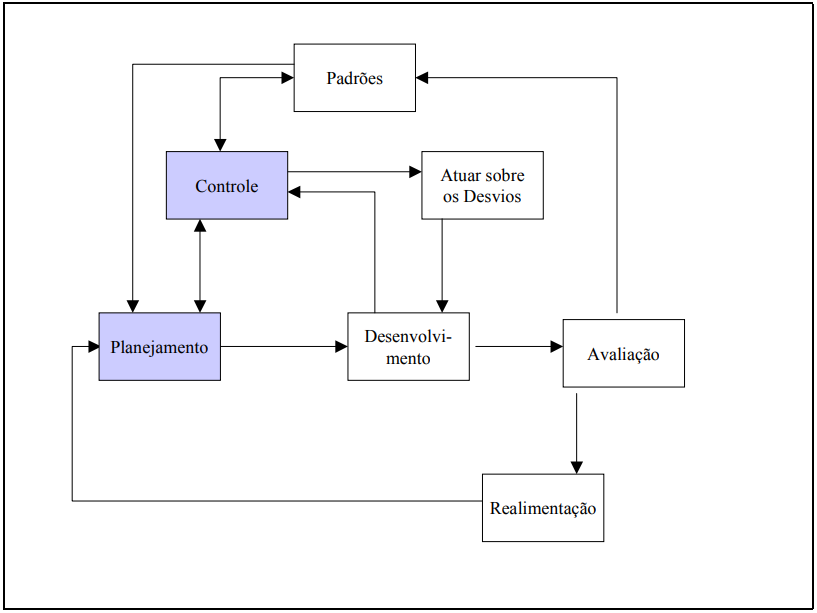
\includegraphics[scale=0.45]{./Figuras/planejamento_projeto.png}
	\end{center}
	\legend{Fonte: \cite{Maria_Isabel_2001}}
\end{figure}

\section{UML}

\section{RUP}

\section{GIT}
\chapter{Descrição Geral do Sistema}
%---

%---
O Software de gestão empresarial utilizado pela empresa Duas Rodas atualmente é o SAP, nele é controlado todo fluxo operacional e de funcionamento da empresa. O Agil.It trabalhará em conjunto com o SAP no módulo de manutenção de equipamentos, atuando como meio digitalizado e fazendo ponte com o SAP onde irá integrar informações prévias e competentes às ordens de manutenção.

Dividido em duas aplicações independentes, o sistema é capaz de trabalhar de forma autônoma, podendo receber e enviar dados via API ou realizar cadastros manualmente na aplicação WEB. Enquanto no aplicativo será possível acompanhar as ordens, fazer apontamentos e realizar breves consultas.

% CAP 2.1
% ---
\section{Descrição do Problema}
% ---
A gestão do processo de manutenção de máquinas é feita de forma manual, com isso, há bastante retrabalho para repassar todos os dados ao sistema, outra preocupação é o gasto com folhas de papel. Em adendo, não há uma boa análise dos problemas comuns, equipamentos mais problemáticos, eficiência dos técnicos, entre outras.

Como o processo é feito manualmente, há bastante retrabalho por parte dos administradores e líderes do setor em questão. O tempo consumido pelos colaboradores para a correção dos problemas não permite tempo hábil para fazer a análise dos defeitos ocorridos, sendo assim existe uma dificuldade em realizar métricas desde equipamentos problemáticos até ineficiência dos técnicos.

Outra preocupação que objetiva a automatização das ordens de manutenção é o consumo excessivo de papel, pois a tendência das empresas é serem cada vez mais sustentáveis e portanto, ao digitalizar o processo de ordem de manutenção, a empresa Duas Rodas poderá  ter maiores índices de sustentabilidade e alcançar um maior destaque entre as demais empresas.
%---
% CAP 2.2

\subsection{Cenário Atual}
No processo de manutenção de equipamentos, a empresa Duas Rodas emite uma ordem de manutenção pelo SAP. Após a emissão, é impresso um formulário e entregue ao técnico elencado para a realização da manutenção. O técnico então preenche os campos básicos do formulário e depois preenche os campos que detalham as operações realizadas, bem como os componentes utilizados. Ao finalizar a manutenção, são colhidas 3 assinaturas, a do operador da máquina, a do técnico da manutenção e a do líder de manutenção, sendo que cada uma das partes pode negar a assinatura e solicitar alterações na manutenção realizada. Com todas as assinaturas rubricadas, o formulário é enviado a um funcionário administrativo que digitaliza as informações preenchidas no SAP. Além de gerar um retrabalho imenso, há um problema com a caligrafia dos técnicos, o que dificulta a digitalização dos dados. Com o volume atual de manutenções, é inviável manter o fluxo dessa forma. Com isso, entra o projeto Agil It. Atuando como meio digitalizador, faz a ponte entre a manutenção na fábrica e o sistema SAP, fazendo com que não haja mais retrabalho e eliminando totalmente os papeis utilizados nos formulários.


\begin{figure}[H]
	\caption{\label{cenario_atual1}Cenário Atual}
	\begin{center}
		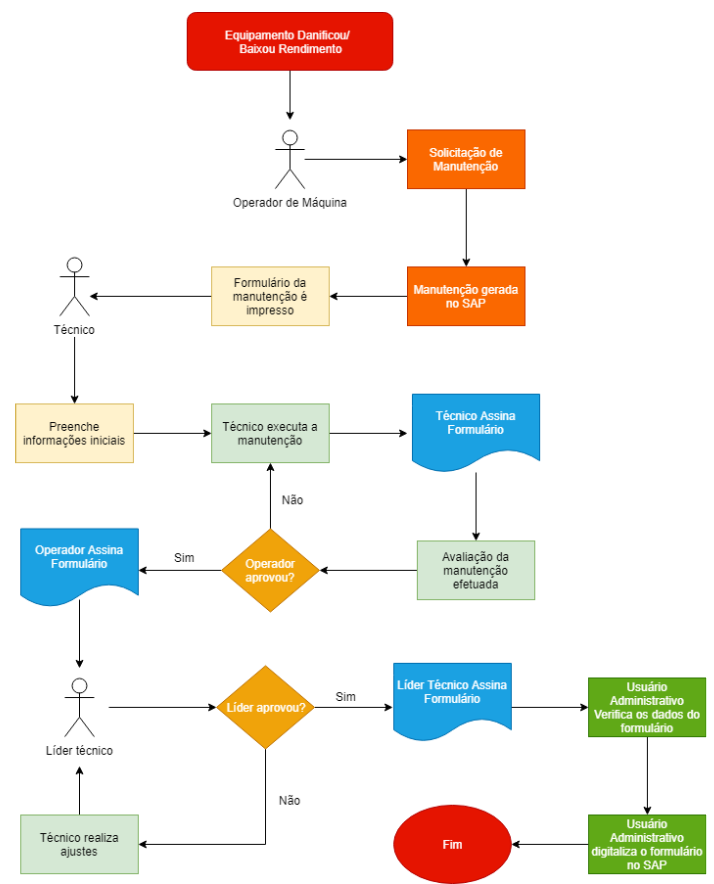
\includegraphics[scale=0.75]{./Figuras/cenario-atual1.png}
	\end{center}
	\legend{Fonte: Os Autores(2020)}
\end{figure}


\subsection{Cenário Com Agil.It}
No processo de manutenção de equipamentos com a Agil.It, a ordem de manutenção será gerada no SAP e os dados serão integrados ao sistema Agil.It. Ao ser integrado, o técnico de manutenção receberá uma notificação informando que tem uma nova OM e ele poderá visualizá-la em seu monitor no aplicativo mobile ou na aplicação WEB. Ele poderá então iniciar a manutenção e fazer os apontamentos das operações e componentes. Após finalizar a manutenção, o técnico assinará a ordem de manutenção. Após isso, o operador do equipamento será notificado e a OM ficará disponível para sua avaliação, podendo este aceitar ou recusar de acordo com as realizações do trabalho. Caso recuse, o operador deve informar o motivo da rejeição ao sistema que então, irá reabrir a OM e solicitar ao técnico para verificar. Caso o operador aceite a execução do trabalho de manutenção, o mesmo deverá assinar a OM e com isto, o sistema notificará o líder técnico, sendo o trabalho deste, averiguar a execução da tarefa, o mesmo também poderá rejeitar e solicitar alterações. Após concluído, ele deve assinar a OM. Com as 3 assinaturas colhidas, o sistema irá notificar o usuário administrador e ele poderá liberar a OM para integração com o SAP.

\begin{figure}[H]
	\caption{\label{figure:cenario_agilit1}Cenário Agil.It}
	\begin{center}
		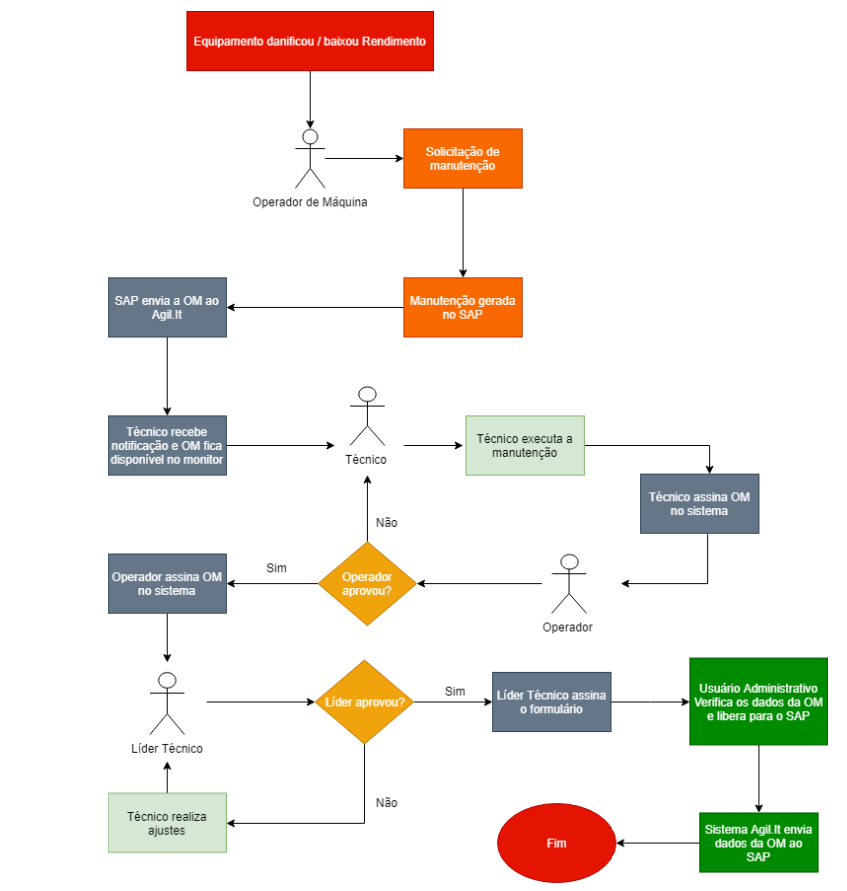
\includegraphics[scale=0.70]{./Figuras/cenario-agilit1.png}
	\end{center}
	\legend{Fonte: os autores (2020)}
\end{figure}
%---
% CAP 2.4
% ---
\section{Principais Envolvidos e suas Características}

% CAP 2.4.1
% ---
\subsection{Usuários do Sistema}
% ---
O Sistema contemplará 4 tipos de usuários, o administrador, o técnico de manutenção, o chefe de manutenção e o operário. Cada usuário terá acessos e funções diferentes no sistema. Todos terão acesso tanto a parte web da aplicação quanto a parte mobile (aplicativo).

\begin{itemize}
	
	\item O usuário administrador será responsável pelos cadastros gerais, poderá consultar e finalizar ordens de manutenção.
	
	\item O técnico de manutenção terá a visão de ordens de manutenção pendentes para ele, podendo iniciar ou pausar alguma a qualquer momento. Após finalizada, poderá realizar a assinatura da ordem.
	
	\item O chefe de manutenção receberá requisições de ordens de manutenção feitas por operadores e irá cadastrar ao sistema. Poderá distribuir as ordens aos técnicos, realizar consultas gerais e assinar as ordens.
	
	\item O operador, que poderá requisitar uma ordem de manutenção ao administrador, acompanhar as ordens solicitadas por ele e assinar a ordem após a conclusão.
	
\end{itemize}
% CAP 2.4.2
% ---
\subsection{Desenvolvedores do Sistema}
% ---

Por trás de todo o desenvolvimento do sistema Agil.It, existe uma equipe de três pessoas formada por Júlio Thomazelli que atua como desenvolvedor na Voce Pede Softwares para Bares e Restaurantes há aproximadamente um ano e meio, com experiência nas tecnologias Angular, Ionic, Object Pascal e Java. A equipe também conta com o desenvolvedor e líder do setor de tickets da startup Clinicorp Solutions, trabalha como fullstack utilizando Node.js no back-end , React.js no front-end e React-Native para dispositivos mobiles há dois anos. Fechando a equipe, a Agil.it possui como gerente de projeto Márcio Henrique Meier, desenvolvedor na empresa Adapcon Processamento de Dados com grande experiência com as linguagens de programação Caché, Vue.js e Node.js, vivencia a área há exatamente três anos.
Os três desenvolvedores são formados como Técnico em Desenvolvimento de Software e acadêmicos do sexto semestre do Tecnólogo em Sistemas para Internet na faculdade Senai de Jaraguá do Sul.

\begin{table}[H]
	\centering
	\caption{\label{tabela_desenvolvedores}Tabela de desenvolvedores Agil.It}
	\begin{tabular}{|l|l|}
		\hline
		\textbf{Desenvolvedor} & \textbf{Atividade}    \\ \hline
		Julio                  & Aplicativo Mobile     \\ \hline
		Lucas                  & Aplicativo Web        \\ \hline
		Márcio                 & Back End / Integração \\ \hline
	\end{tabular}
	\legend{Fonte: os autores (2020)}
\end{table}



\section{Regras de Negócio}
% ---
No contexto da Engenharia de Software as Regras de Negócios são tratadas como alguns requisitos de software, pois sem elas, o software não existiria. Regras de negócio são premissas e restrições aplicadas a uma operação comercial de uma empresa, que precisam ser atendidas para que o negócio funcione da maneira esperada \cite{crerie2008identificacao}.

Segundo \cite{2001SilviaInes} Regras de negócios são mais que declarações sobre campos de dados ou implementação do sistema, elas definem tarefas dos atores da organização, os serviços que a organização dispõem e os recursos necessários para apoiar os processos do negócio.

Já \cite{1997kilovSimmonds} são mais enfáticos, para eles uma regra de negócio deve ser objetiva e definida em termos de notações matemáticas de proposições, mostrando que precisão é essencial quando formula-se as regras de negócio. Uma proposição é um fato ou estado observável de negócio envolvendo uma ou mais entidades pelo qual é possível afirmar ou negar a vericidade dessas entidades.

Desta forma as regras de negócio da empresa de Alimentos Duas Rodas seriam:

\begin{subalineas}
	\item {Os administradores, líderes de manutenção e líderes de setor poderão criar ordens de manutenção};
	\item {Apenas o administrador poderá finalizar ordens de manutenção};
	\item {Os cadastros só serão possíveis na versão web};
	\item {Cada ordem de manutenção deve conter uma assinatura do técnico de manutenção, uma do operador ou líder de setor e uma do administrador};
	\item {Cada ordem de manutenção só pode ser finalizada após ter as 3 assinaturas};
	\item {Somente administradores terão acesso à tela de pendência de assinaturas};
	\item {Cada técnico de manutenção só pode ter uma ordem iniciada por vez};
	\item {Técnicos de manutenção podem pausar ordens de manutenção};
	\item {Técnicos de manutenção podem ter várias ordens pausadas ao mesmo tempo};
	\item {Pode haver mais de um técnico de manutenção por ordem de manutenção};
	\item {Uma ordem deve ter um técnico de manutenção principal};
\end{subalineas}




% ---
\chapter{Requisitos do Sistema}
Os requisitos são capacidades que devem ser atendidas ou possuídas por um sistema para resolver um problema ou atingir um objetivo, O conjunto de todos os requisitos que formam a base para o desenvolvimento subsequente de um software \cite{vazquez2016}. Neles são definidos como serão os comportamentos do sistema e seus fluxos. Eles serão abordados em dois segmentos: Os Requisitos funcionais que são fluxos do sistema e os requisitos não funcionais que são necessários para a utilização do sistema.

\section{Requisitos Funcionais}

{ Conforme \cite{essi2005}, requisitos funcionais são as necessidades descritas pelo cliente, onde a equipe do projeto analisa e
especifica as funções, desempenho, interfaces e restrições, conforme as fases das metodologias aplicadas. Sua finalidade é disntringuir as dependências do sistema para que o mesmo funcione de acordo com os requisitos informados pelo cliente. }

\subsection{Cadastros}


\begin{subalineas}
	\item {Usuários};
	\item {Setores};
	\item {Máquinas};
	\item {Unidades de medida};
	\item {Peças};
	\item {Tipos de estoques};
	\item {Estoque de peças};
	\item {Ordem de manutenção}.
\end{subalineas}

\subsection{Consultas}
\begin{subalineas}
	\item {Máquinas};
	\item {Estoque de peças};
	\item {Ordem de manutenção};
	\item {Login};
	\item {Logoff}.
\end{subalineas}

\subsection{Funcionalidades}
\begin{subalineas}
	\item {Monitor de ordens em aberto};
	\item {Solicitação de abertura de ordem de manutenção};
	\item {Central de notificação}.
\end{subalineas}

\section{Requisitos Não Funcionais}

{\cite{IIBA2005} relata que o propósito dos requisitos não funcionais é descrever as qualidades requeridas para um sistema, como sua usabilidade e seu desempenho. Em sistemas alguns destes requisitos podem determinar tecnologias ou algoritmos específicos a serem utilizados, garantindo compatibilidade com sistemas existentes \cite{cordeiro2007}

\subsection{Funcionalidades}
\begin{subalineas}
	\item {Sistema desenvolvido para web};
	\item {Utilizar o banco MS Sql Server};
	\item {Usuários devem ter acesso à computadores e/ou dispositivos móveis}.
\end{subalineas}

\section{Fluxograma do Sistema Desenvolvido}

{Segundo \cite{pejeronimo2002} fluxograma é uma representação gráfica das tarefas de um determinado processo, sendo de forma sequencial a execução delas. \cite{roberthurt} relata que um fluxograma fornece um panorama de alto nível sobre um sistema de informação.

\newpage
\begin{figure}[htb]
	\caption{\label{flux_sys}Fluxo do AGIL.IT}
	\begin{center}
		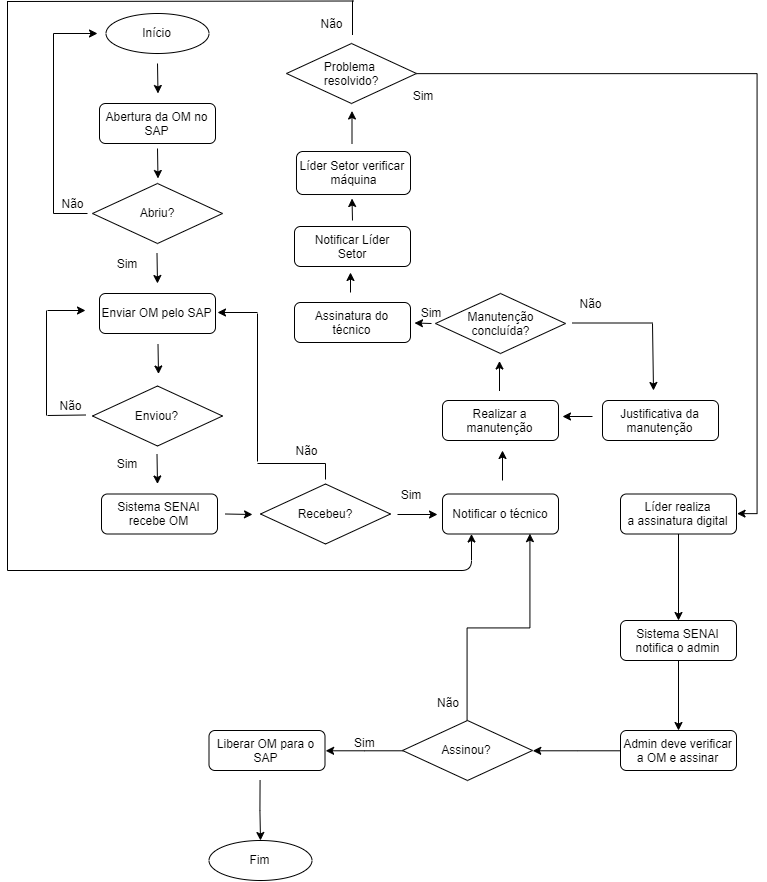
\includegraphics[scale=0.55]{./Figuras/fluxo-sistema.png}
	\end{center}
	\legend{Fonte: Próprio Autor, 2019}
\end{figure}

Na Figura \ref{flux_sys} é possível verificar todo o fluxo do sistema onde começa e termina com a integração do SAP.
O sistema irá receber a OM do SAP e notificar o técnico. Após o técnico realizar a manutenção os usuários realizam as assinaturas e o usuário administrador analisa e libera a OM para a integração.


\section{Diagrama de Caso de Uso do Sistema }

{Diagramas dos casos de uso são técnicas utilizadas para captar os requisitos funcionais de um sistema, descrevem as interações entre usuários de um sistema e o próprio sistema, fornecendo uma narrativa sobre como ele é utilizado \cite{umlessencial2005}. Para \cite{carniello2003} seu objetivo principal consiste em definir o comportamento de um sistema, sem revelar sua estrutura interna.}

\newpage
\begin{figure}[htb]
	\caption{\label{caso_uso}Caso de Uso do AGIL.IT}
	\begin{center}
		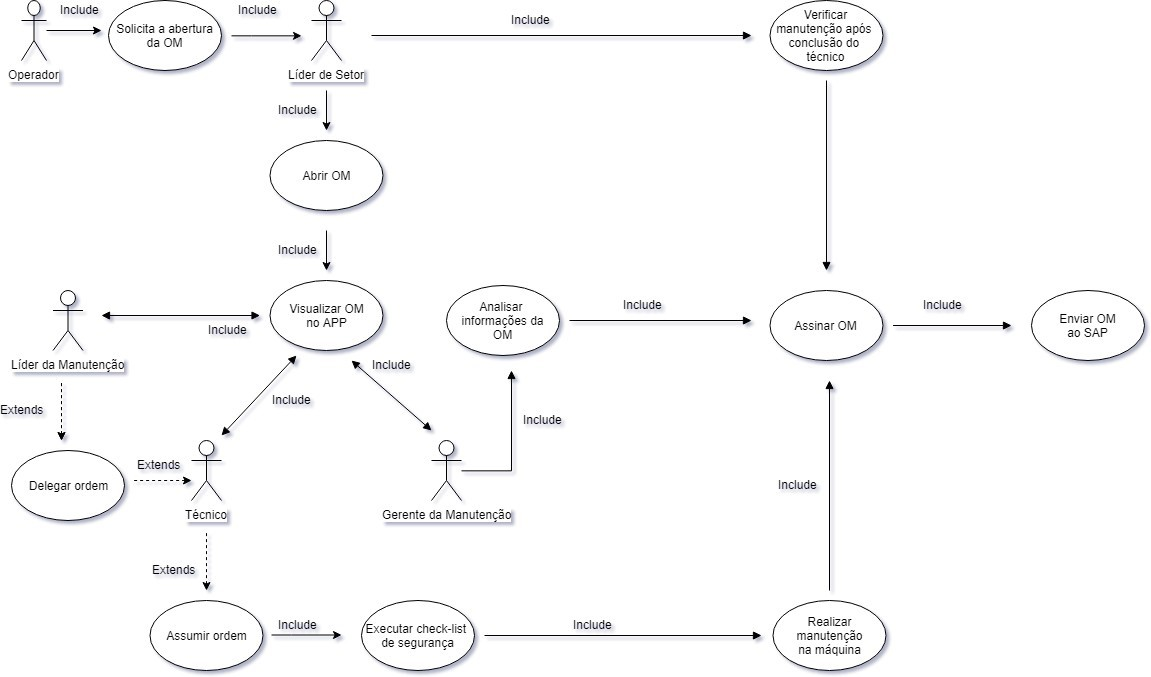
\includegraphics[scale=0.50]{./Figuras/caso-uso.png}
	\end{center}
	\legend{Fonte: Próprio Autor, 2019}
\end{figure}

Na Figura \ref{caso_uso} é possível verificar quais ações cada ator desempenhará no sistema.
Os operadores de máquinas e os líderes de manutenção verificam a manutenção feita e assinam a OM. O técnico realizará a manutenção e verificará as peças necessárias para realizar a assistência ao equipamento e se as mesmas possuem estoque disponível. E o administrador realizará cadastros e encerará as ordens de manutenção.


\section{Entidade de Relacionamento do Banco de Dados}

{Planejar todas as etapas, dedicando a atenção especialmente ao projeto de estruturação do banco de dados. Com a estrutura pronta, a facilidade para dar manutenção no sistema fica muito mais fácil.
Tem como objetivo, obter uma descrição de forma abstrata dos dados que serão armazenados no banco de dados \cite{2010_erbd}. }


\newpage
\begin{figure}[htb]
	\caption{\label{entidade_relacionamento}Entidade de Relacionamento}
	\begin{center}
		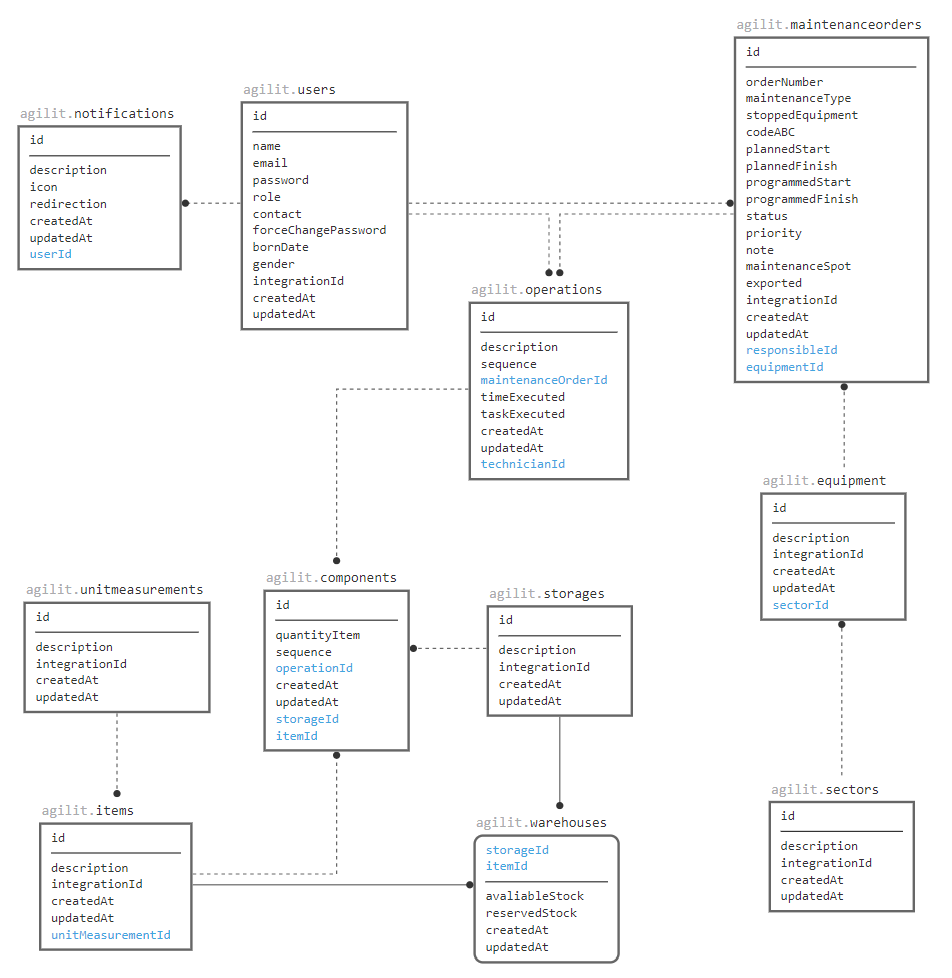
\includegraphics[scale=0.70]{./Figuras/er3.png}
	\end{center}
	\legend{Fonte: Próprio Autor, 2019}
\end{figure}

A Figura \ref{entidade_relacionamento} mostra toda a entidade de relacionamento do banco de dados, onde cada tabela representa uma estrutura de dados no banco de dados e as ligações entre elas demonstram relacionamentos que essas tabelas possuem entre si.


\newpage
\section{Cronograma do Projeto}


Todo bom projeto deve ter um cronograma e um planejamento de ação, baseado nisso, foi elaborado dois cronogramas: um apresentando todo o conteúdo aprendido no semestre e outro montando plano de ação para implementação do projeto.

As figuras a seguir, são cronogramas que demonstram a trajetória do desenvolvimento do projeto. Divididos por semestre, os cronogramas listam as atividades aprendidas nas UCs, com todas as partes teóricas e práticas onde o objetivo principal é implementar todo conhecimento adquirido em prol de um projeto único: A unificação de todas as UCs do curso de Sistemas para Internet.

\begin{figure}[htb]
	\caption{\label{cron-3-semestre}Cronograma de Aprendizagem: Terceiro Semestre}
	\begin{center}
		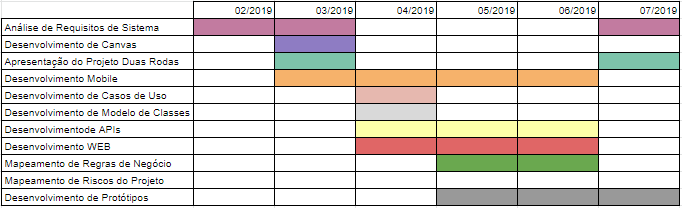
\includegraphics[scale=0.90]{./Figuras/cronograma-3-semestre.png}
	\end{center}
\end{figure}


\begin{figure}[htb]
	\caption{\label{cron-4-semestre}Cronograma de Aprendizagem: Quarto Semestre}
	\begin{center}
		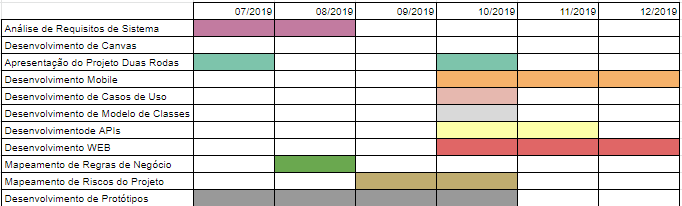
\includegraphics[scale=0.90]{./Figuras/cronograma-4-semestre.png}
	\end{center}
\end{figure}


\begin{figure}[htb]
	\caption{\label{cron-4-semestre}Cronograma de Aprendizagem: Quinto Semestre}
	\begin{center}
		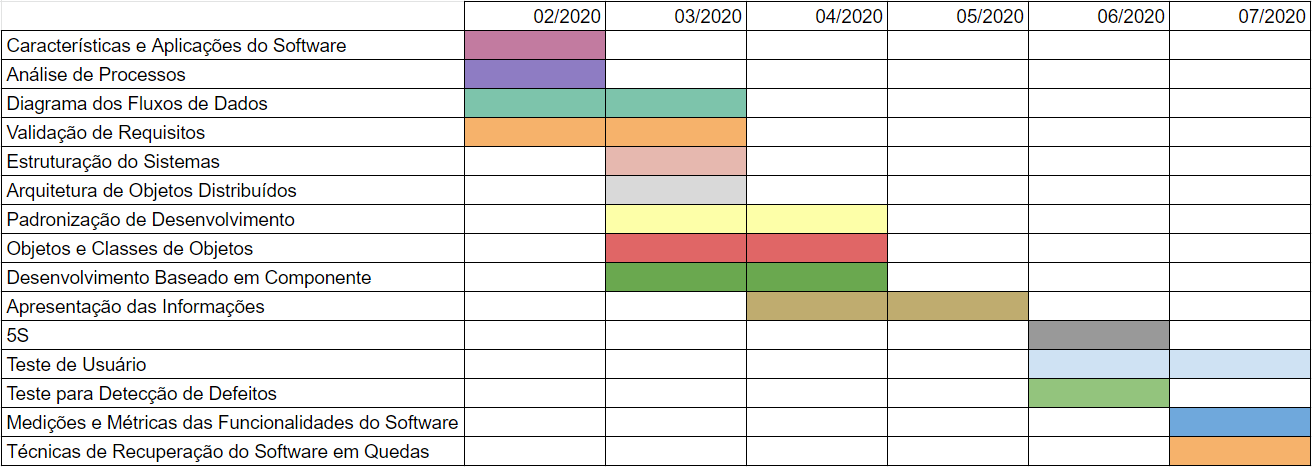
\includegraphics[scale=0.70]{./Figuras/cronograma-5-semestre.png}
	\end{center}
\end{figure}
\chapter{Protótipo}
A prototipação é uma etapa de suma importância no desenvolvimento de projeto de software. Além de melhorar a produtividade da equipe, ela facilita o entendimento dos requisitos do sistema e permite a apresentação de de conceitos e funcionalidades da aplicação de modo simplificado.
Nesse trabalho foi utilizado a prototipação visual cujo ênfase se aplica a estética e usabilidade. Nesse tipo de protótipo é possível identificar o layout e a identidade visual da aplicação. \cite{dextra2013prototipacao}

\section{Aplicação WEB}
A aplicação web tem como foco o gerenciamento de toda a aplicação envolvendo consultas e cadastros gerais do sistema.
Apesar desse foco acentuado à gestão, é possível desempenhar todos os papeis dentro da aplicação web.

\newpage
\subsection{Login}

\begin{figure}[htb]
	\caption{\label{web_login}Tela de Login do Agil.It}
	\begin{center}
		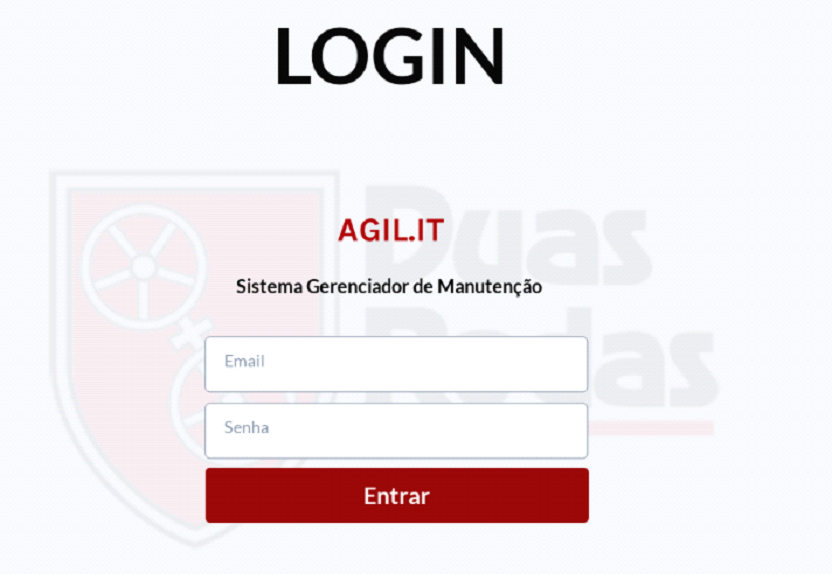
\includegraphics[scale=0.70]{./Figuras/web/login.png}
	\end{center}
	\legend{Fonte: Próprio Autor, 2019}
\end{figure}

A tela \ref{web_login} será a página responsável por autenticar os usuários e garantir a segurança do sistema.

\newpage
\subsection{Configurações do Sistema}

\begin{figure}[htb]
	\caption{\label{web_configuracao}Configuração do Sistema}
	\begin{center}
		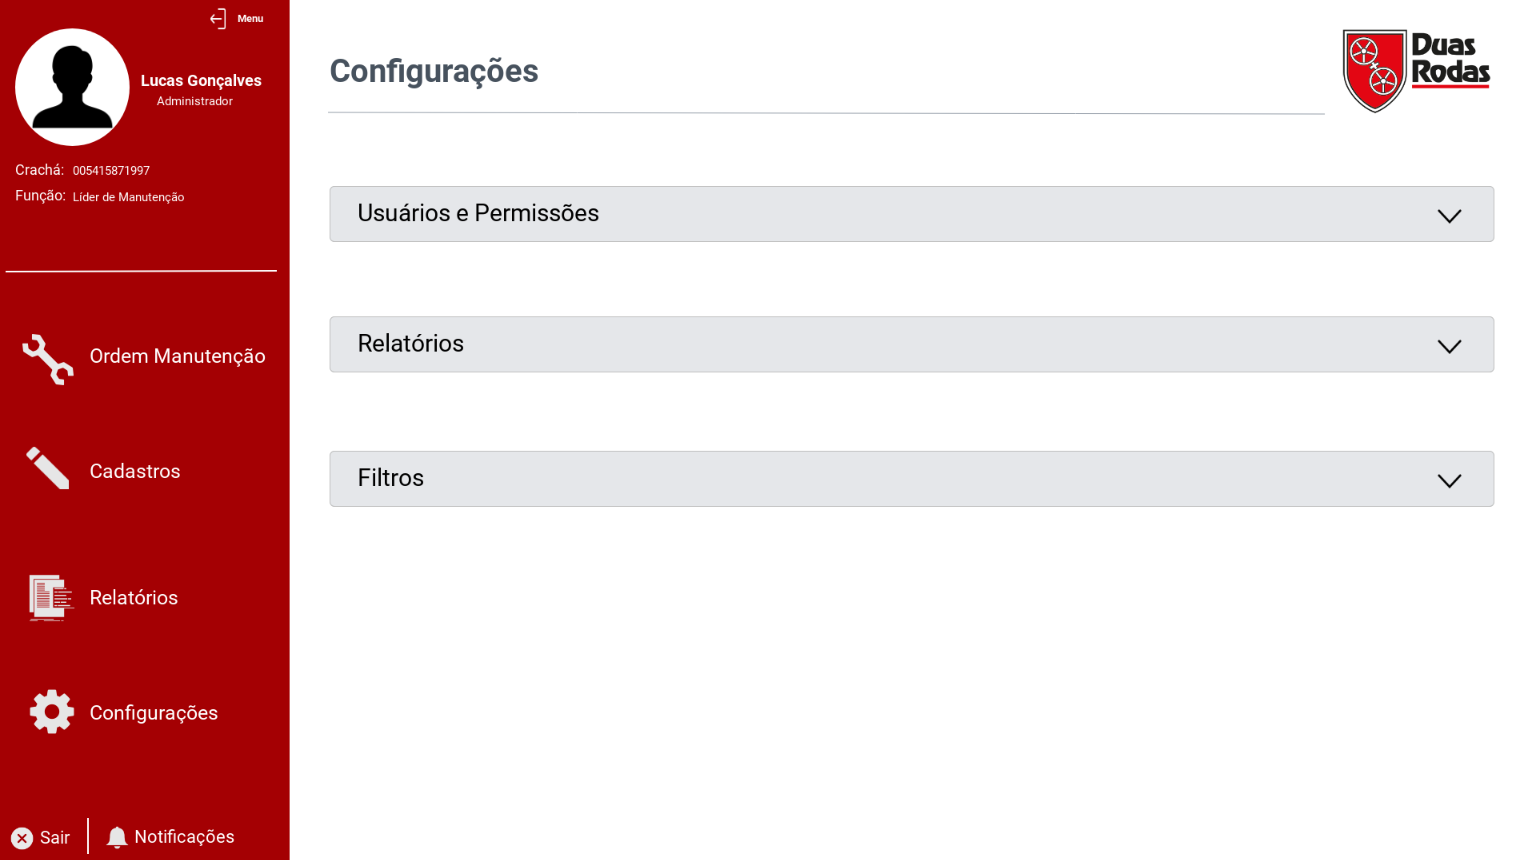
\includegraphics[scale=0.40]{./Figuras/web/configuracoes.png}
	\end{center}
	\legend{Fonte: Próprio Autor, 2019}
\end{figure}

Na tela \ref{web_configuracao} é possível configurar os níveis de acessos dos usuários dentro do sistema bem como quais campos o usuário tem acesso em relatórios e em filtros de tela.

\newpage
\subsection{Cadastro de Usuário}

\begin{figure}[htb]
	\caption{\label{web_cad-user}Cadastro de Usuários}
	\begin{center}
		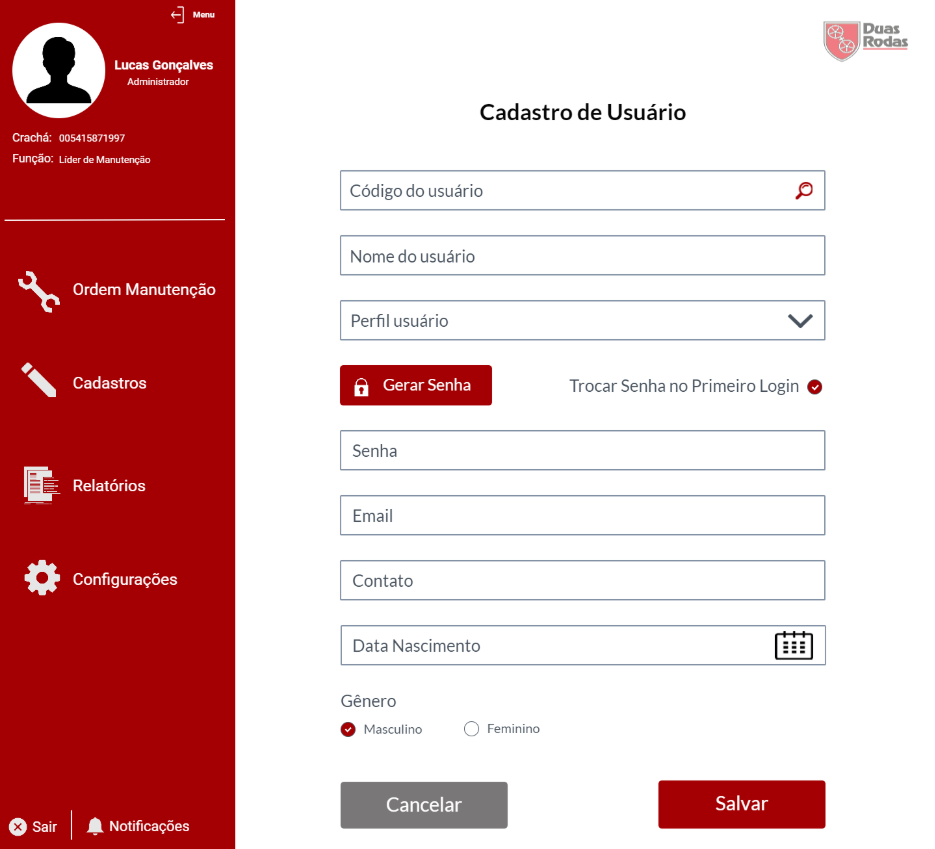
\includegraphics[scale=0.70]{./Figuras/web/cad-user.png}
	\end{center}
	\legend{Fonte: Próprio Autor, 2019}
\end{figure}

Na tela \ref{web_cad-user} será possível cadastrar usuários que utilizarão o sistema.

\newpage
\subsection{Cadastro de Tipo de Máquina}

\begin{figure}[htb]
	\caption{\label{web_cad-tipo-maquina}Cadastro de Tipo de Máquina}
	\begin{center}
		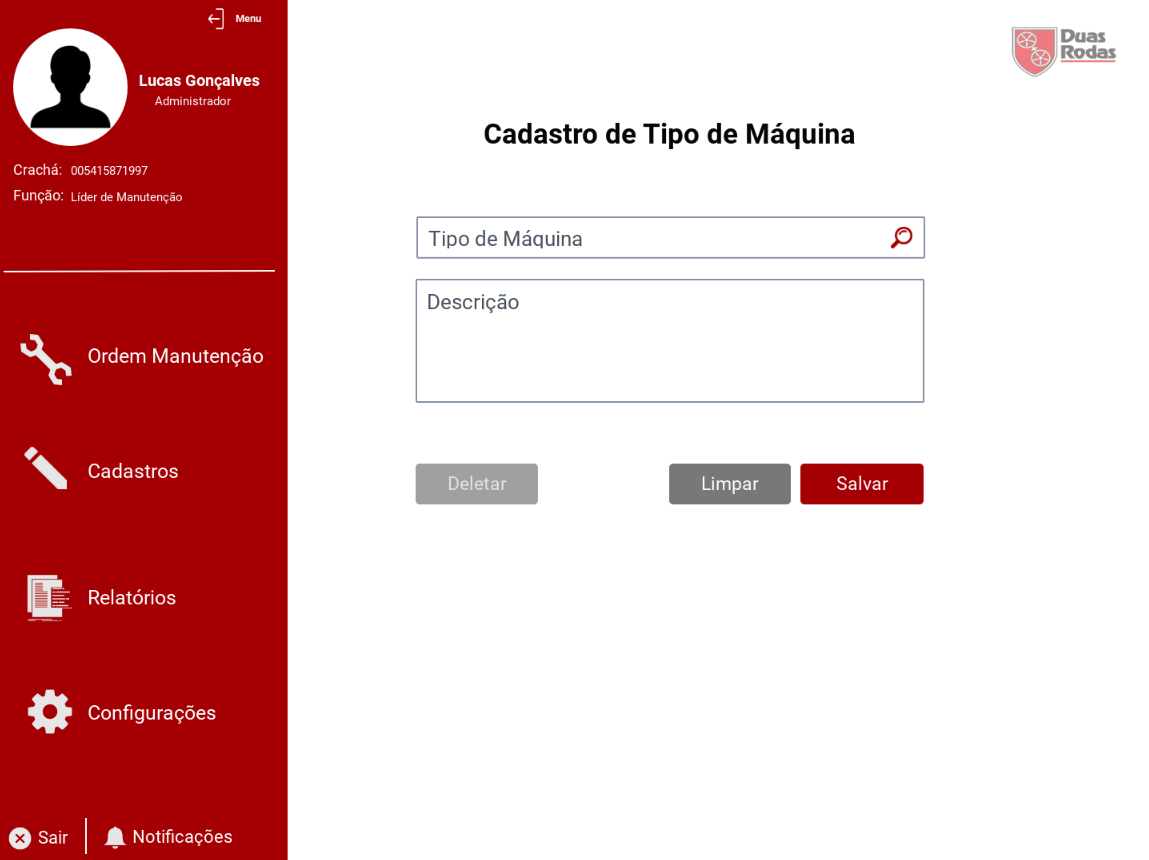
\includegraphics[scale=0.55]{./Figuras/web/cad-tipo-maquina.png}
	\end{center}
	\legend{Fonte: Próprio Autor, 2019}
\end{figure}

Na tela \ref{web_cad-tipo-maquina} é possível cadastrar o tipo de máquina.

\newpage
\subsection{Cadastro de Componente de Máquina}

\begin{figure}[htb]
	\caption{\label{web_cad-componente-maquina}Cadastro de Componente de Máquina}
	\begin{center}
		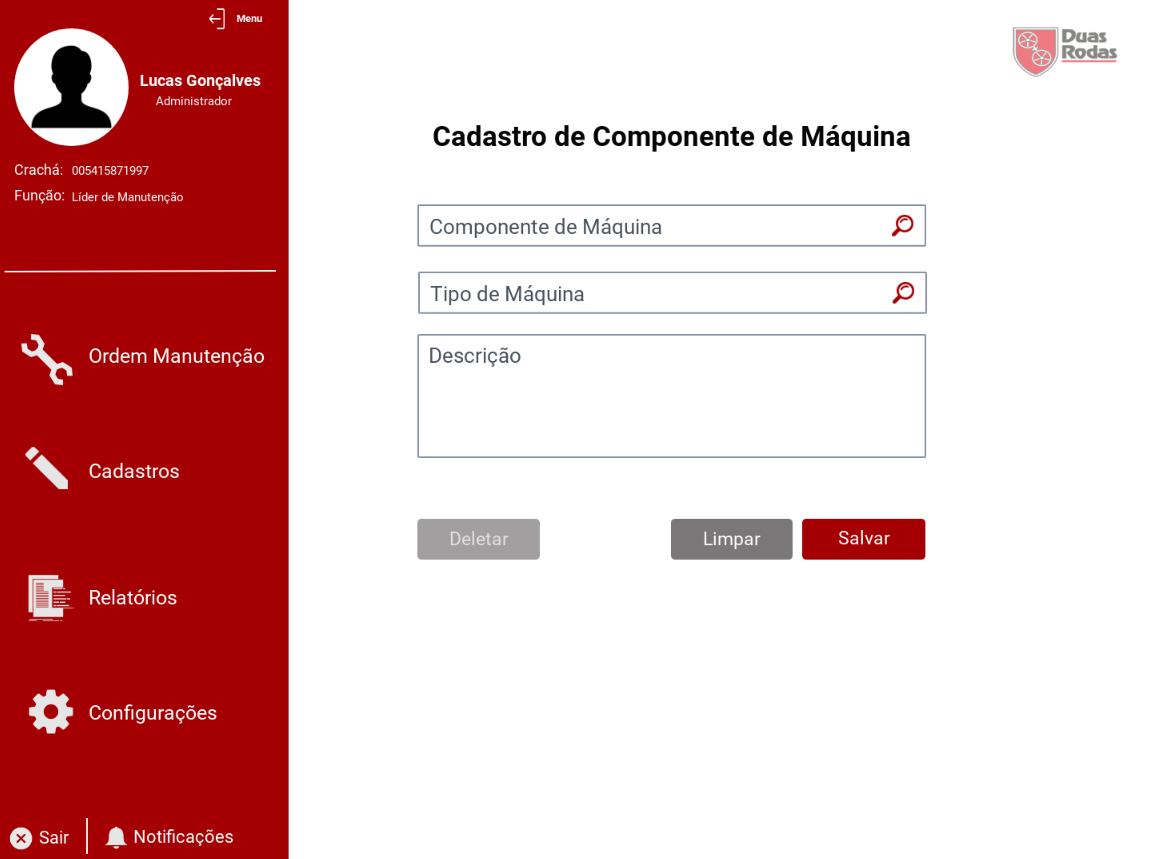
\includegraphics[scale=0.55]{./Figuras/web/cad-componente-maquina.png}
	\end{center}
	\legend{Fonte: Próprio Autor, 2019}
\end{figure}

Na tela \ref{web_cad-componente-maquina} é possível cadastrar os componentes da máquina.

\newpage
\subsection{Cadastro de Setor}

\begin{figure}[htb]
	\caption{\label{web_cad-setor}Cadastro de Setor}
	\begin{center}
		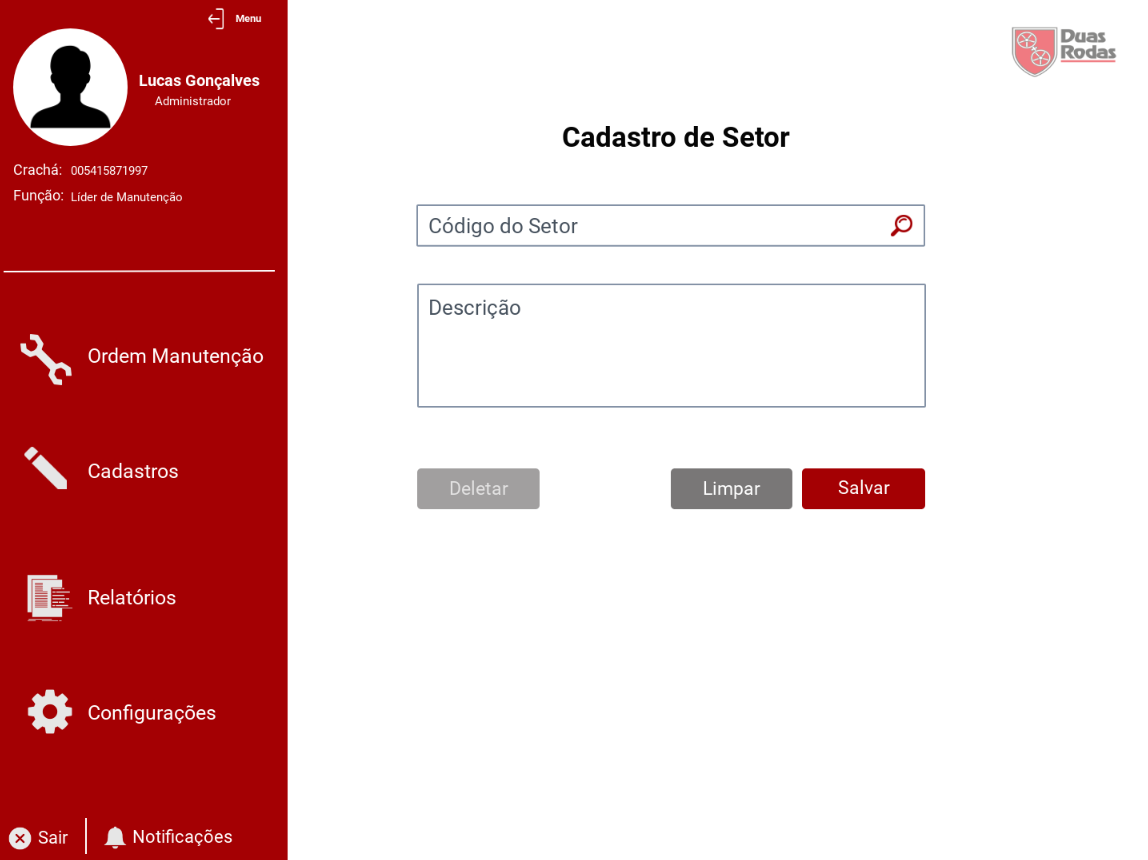
\includegraphics[scale=0.55]{./Figuras/web/cad-setor.png}
	\end{center}
	\legend{Fonte: Próprio Autor, 2019}
\end{figure}

Na tela \ref{web_cad-setor} será possível cadastrar setores. Campo utilizado para identificar a localidade do equipamento.

\newpage
\subsection{Cadastro de Equipamento}

\begin{figure}[htb]
	\caption{\label{web_cad-equip}Cadastro de Equipamento}
	\begin{center}
		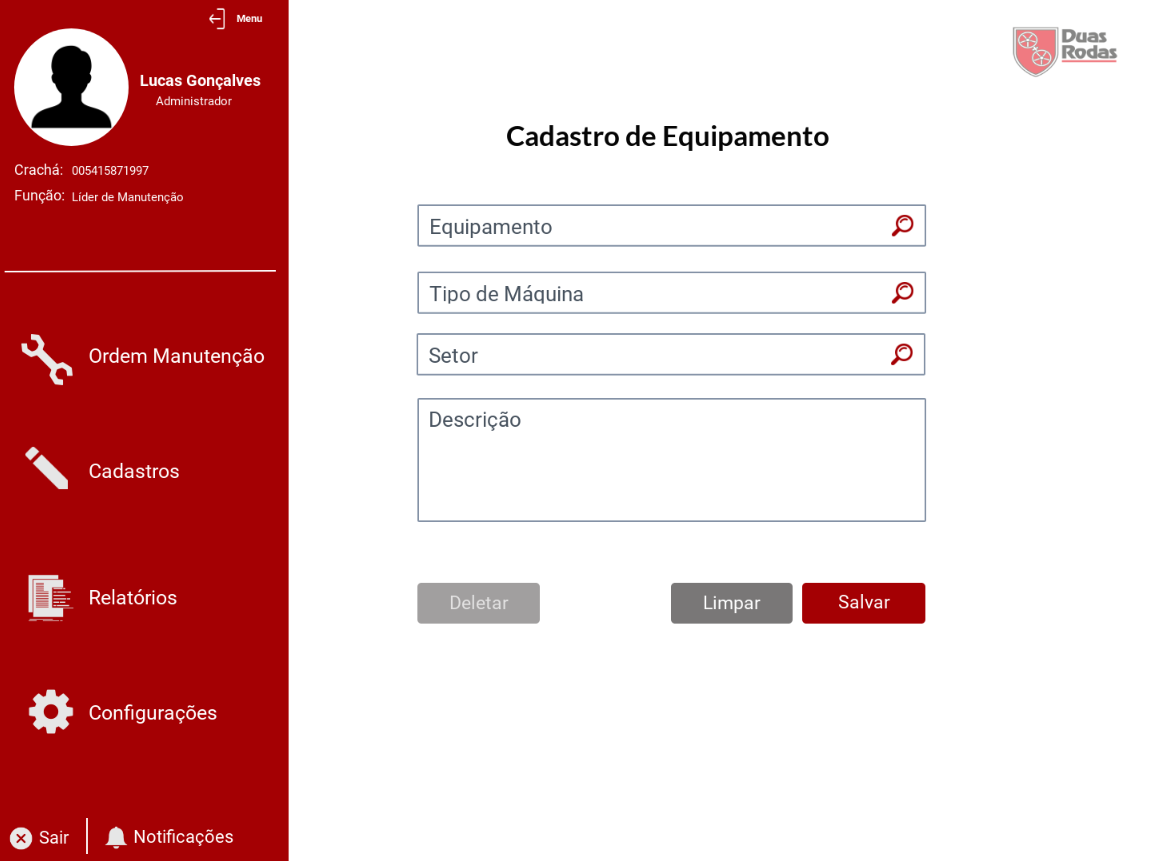
\includegraphics[scale=0.55]{./Figuras/web/cad-equip.png}
	\end{center}
	\legend{Fonte: Próprio Autor, 2019}
\end{figure}

Na tela \ref{web_cad-equip} será possível cadastrar equipamentos.

\newpage
\subsection{Cadastro de Unidade de Medida}

\begin{figure}[htb]
	\caption{\label{web_cad-uni-med}Cadastro de Unidade de Medida}
	\begin{center}
		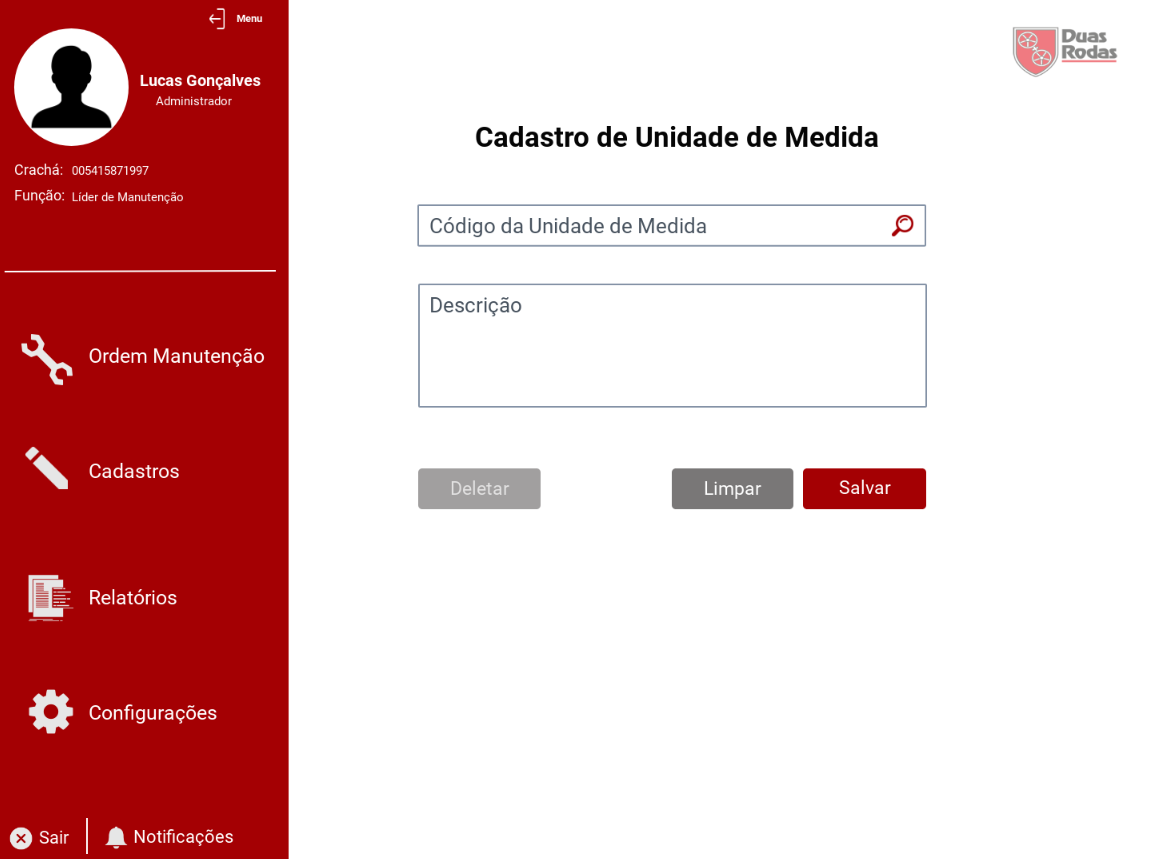
\includegraphics[scale=0.55]{./Figuras/web/cad-uni-med.png}
	\end{center}
	\legend{Fonte: Próprio Autor, 2019}
\end{figure}

Na tela \ref{web_cad-uni-med} será possível cadastrar unidades de medida. Campo utilizado nas peças.

\newpage
\subsection{Cadastro de Peça}

\begin{figure}[htb]
	\caption{\label{web_cad-peca}Cadastro de Peça}
	\begin{center}
		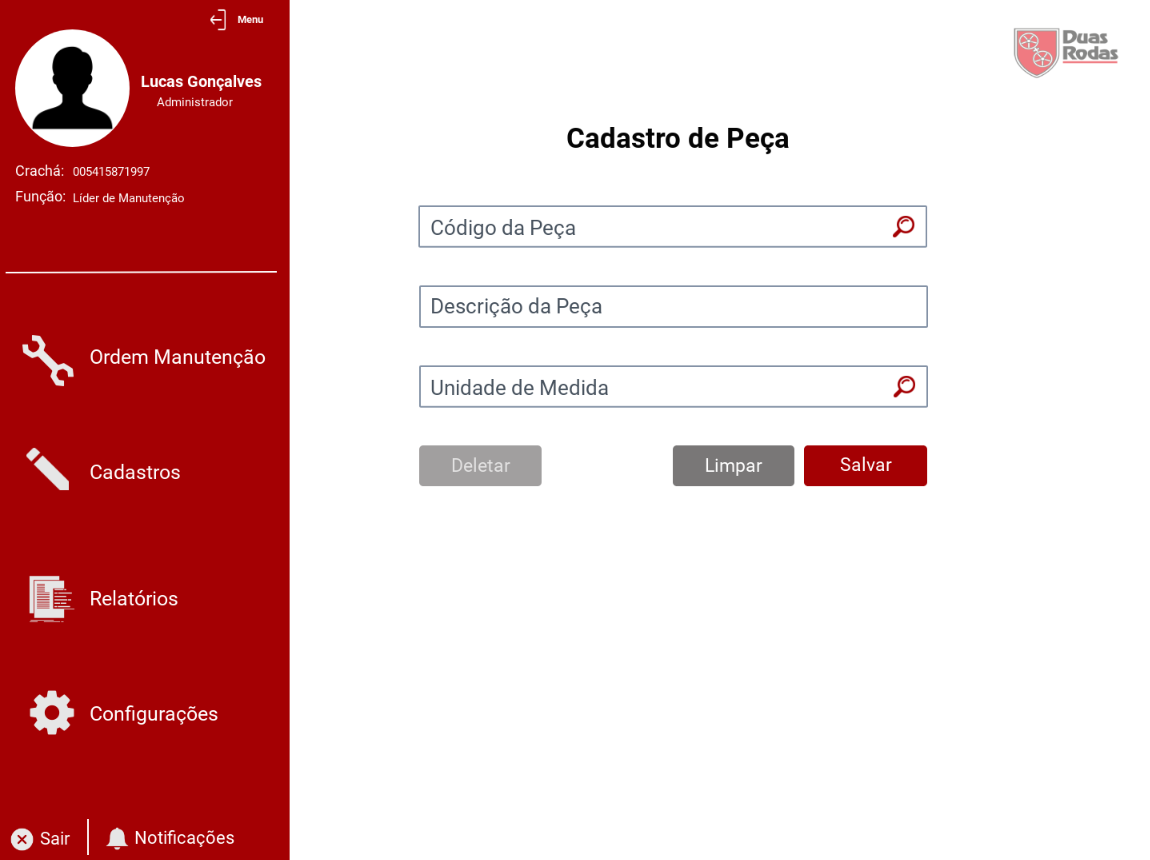
\includegraphics[scale=0.55]{./Figuras/web/cad-peca.png}
	\end{center}
	\legend{Fonte: Próprio Autor, 2019}
\end{figure}

Na tela \ref{web_cad-peca} será possível cadastrar peças que serão utilizadas na manutenção dos equipamentos.

\newpage
\subsection{Cadastro de Local de Estoque}

\begin{figure}[htb]
	\caption{\label{web_cad-loc-estoque}Cadastro de Local de Estoque}
	\begin{center}
		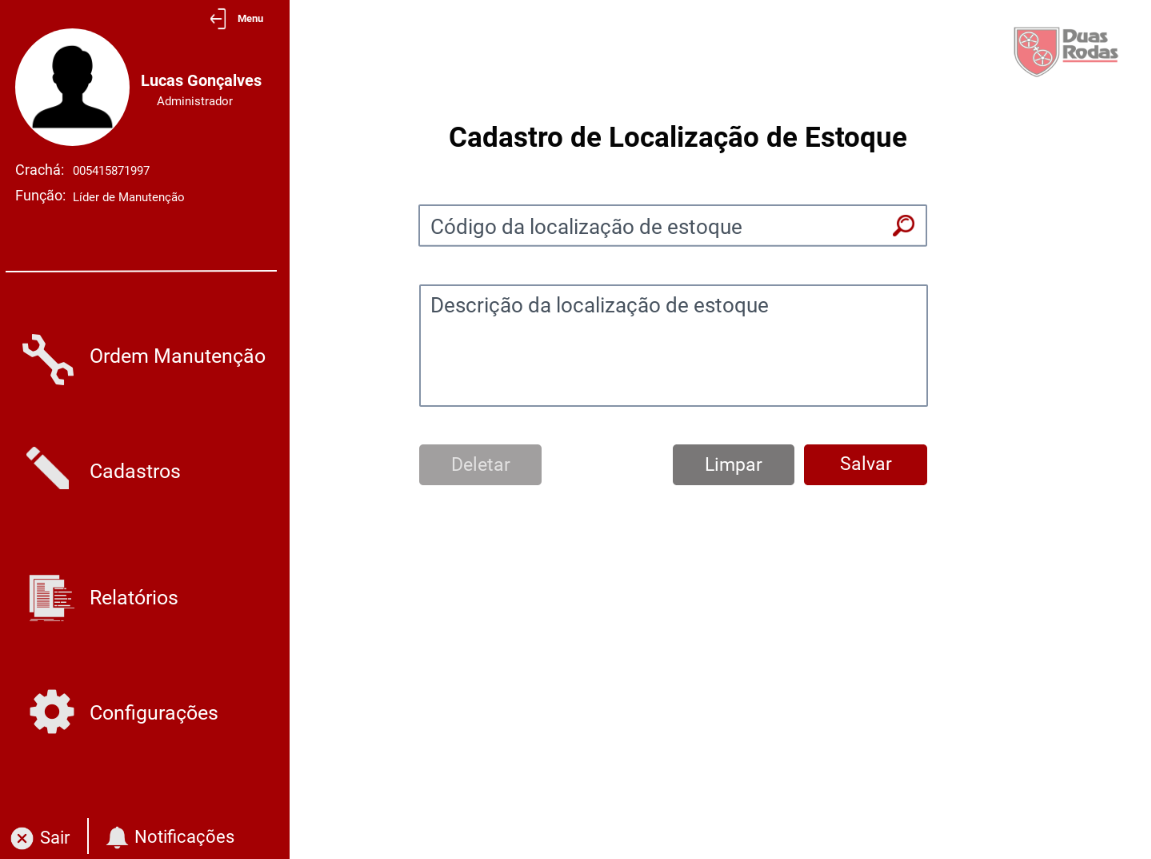
\includegraphics[scale=0.55]{./Figuras/web/cad-loc-estoque.png}
	\end{center}
	\legend{Fonte: Próprio Autor, 2019}
\end{figure}

Na tela \ref{web_cad-loc-estoque} será possível cadastrar localidades de estoque. Essas localidades são um gerenciamento lógico de estoques.

\newpage
\subsection{Atualização de Estoque de Peça}

\begin{figure}[htb]
	\caption{\label{web_est-estoque}Atualização de Estoque de Peça}
	\begin{center}
		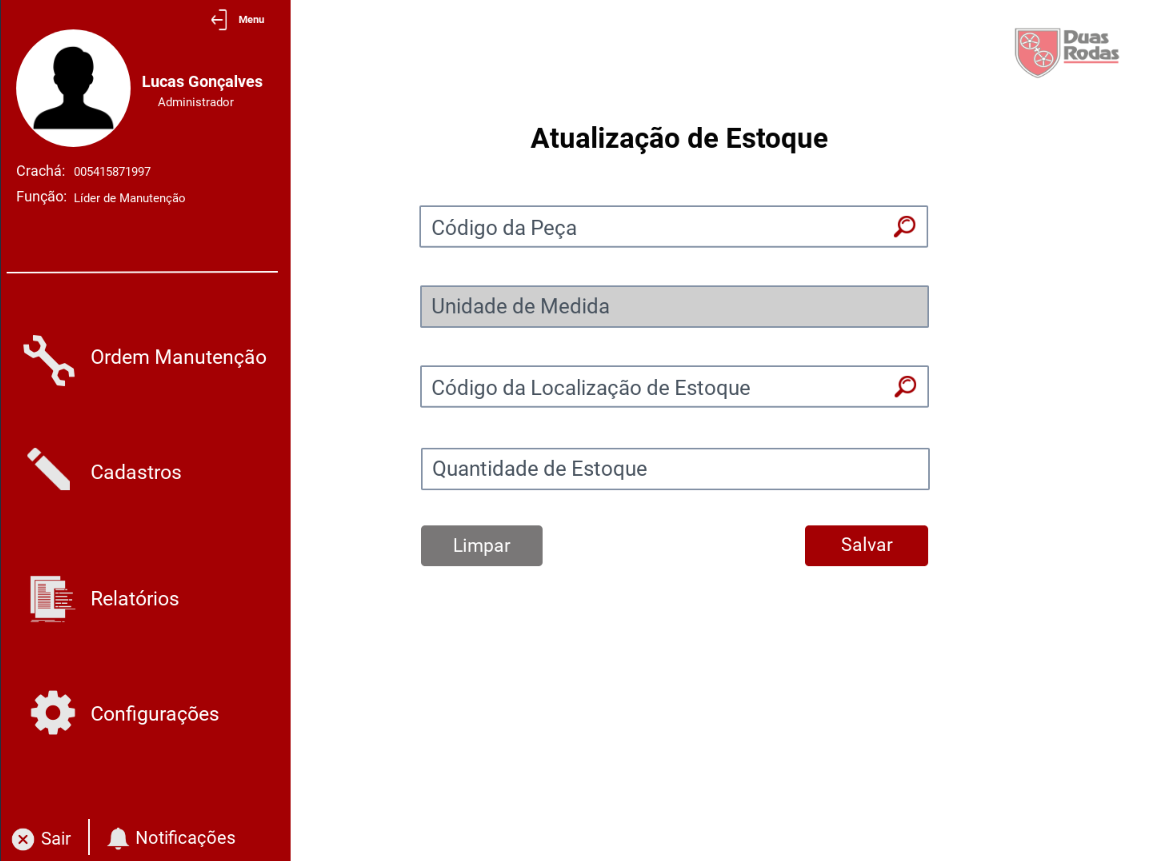
\includegraphics[scale=0.55]{./Figuras/web/est-estoque.png}
	\end{center}
	\legend{Fonte: Próprio Autor, 2019}
\end{figure}

Na tela \ref{web_est-estoque} será possível atualizar a quantidade de peças em um determinado estoque.

\newpage
\subsection{Cadastro de Causa de Defeito}

\begin{figure}[htb]
	\caption{\label{web_cad-causa-defeito}Cadastro de Causa de Defeito}
	\begin{center}
		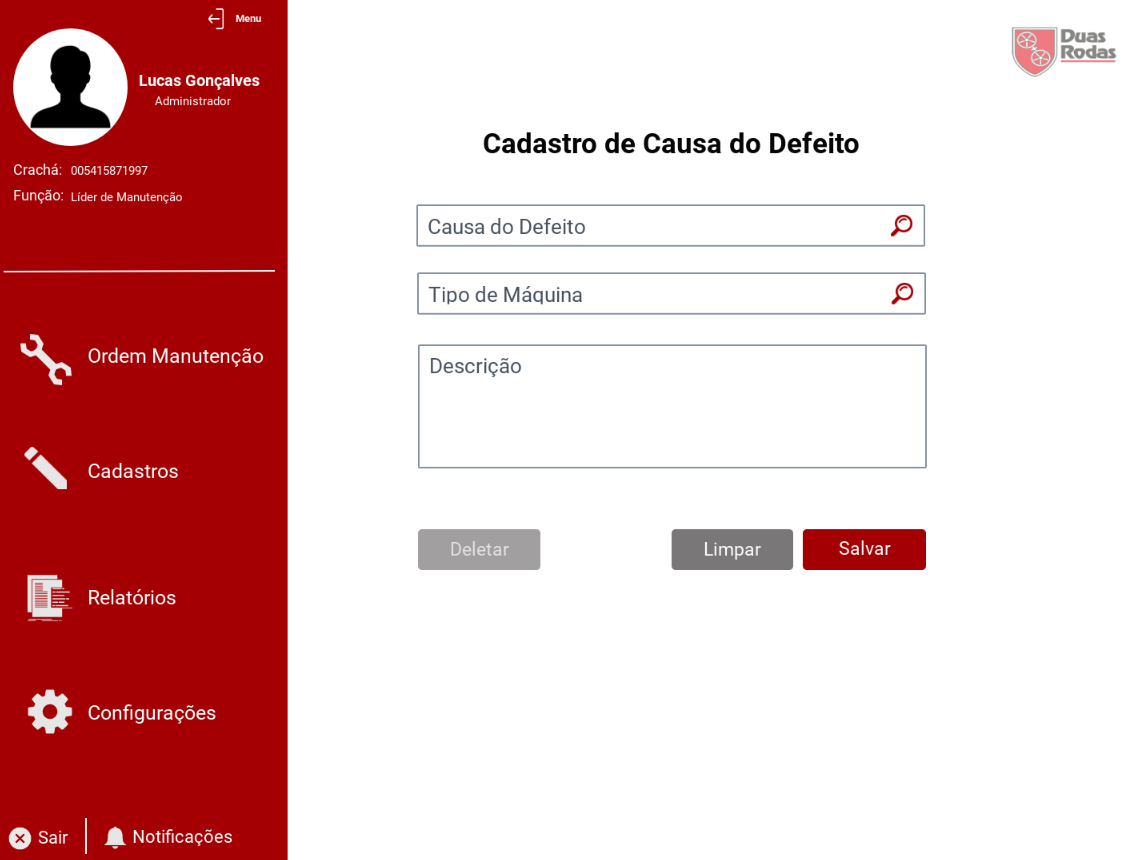
\includegraphics[scale=0.55]{./Figuras/web/cad-causa-defeito.png}
	\end{center}
	\legend{Fonte: Próprio Autor, 2019}
\end{figure}

Na tela \ref{web_cad-causa-defeito} é possível cadastrar as causas do defeito de componentes de equipamentos.

\newpage
	\subsection{Cadastro de Sintoma de Defeito}

\begin{figure}[htb]
	\caption{\label{web_cad-sintoma-defeito}Cadastro de Sintoma de Defeito}
	\begin{center}
		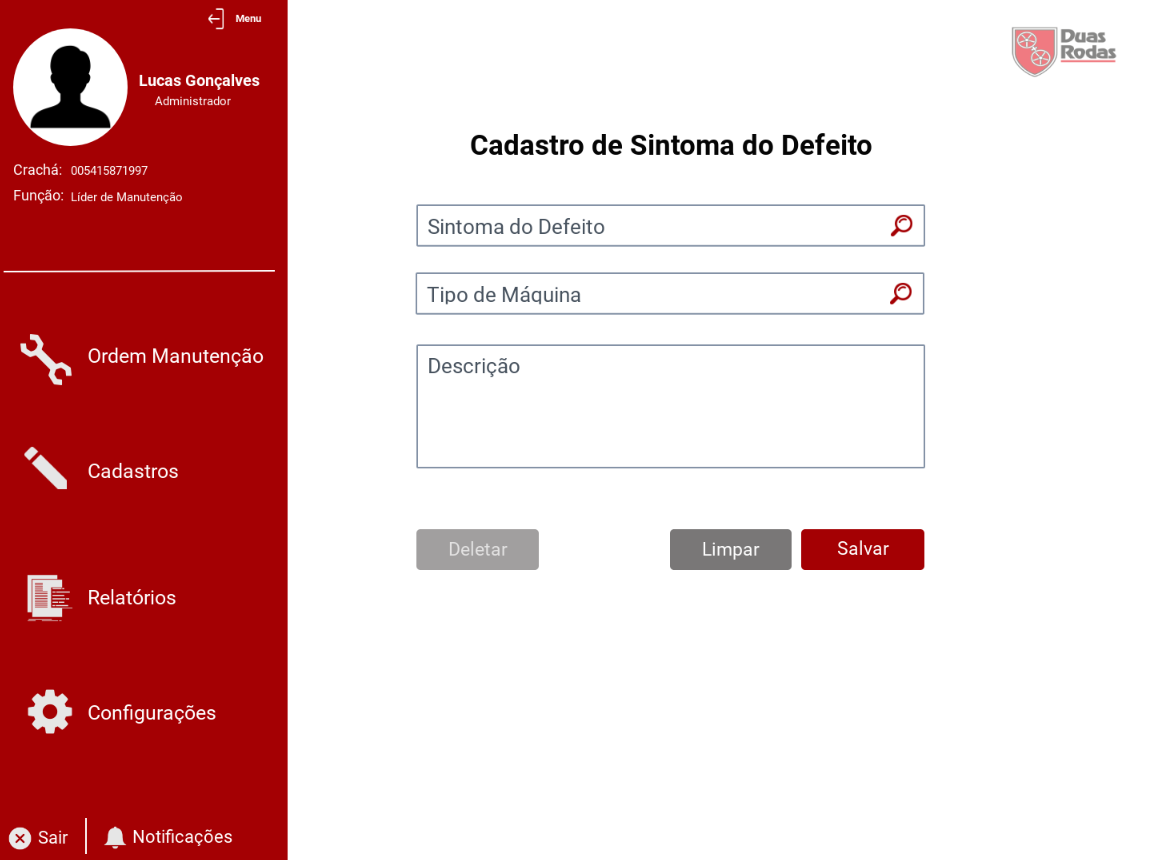
\includegraphics[scale=0.55]{./Figuras/web/cad-sintoma-defeito.png}
	\end{center}
	\legend{Fonte: Próprio Autor, 2019}
\end{figure}

Na tela \ref{web_cad-sintoma-defeito} é possível cadastrar os sintomas dos componentes dos equipamentos.

\newpage
\subsection{Cadastro de Classificação de Ordem de Manutenção}

\begin{figure}[htb]
	\caption{\label{web_cad-classificacao-om}Cadastro de Classificação de Ordem de Manutenção}
	\begin{center}
		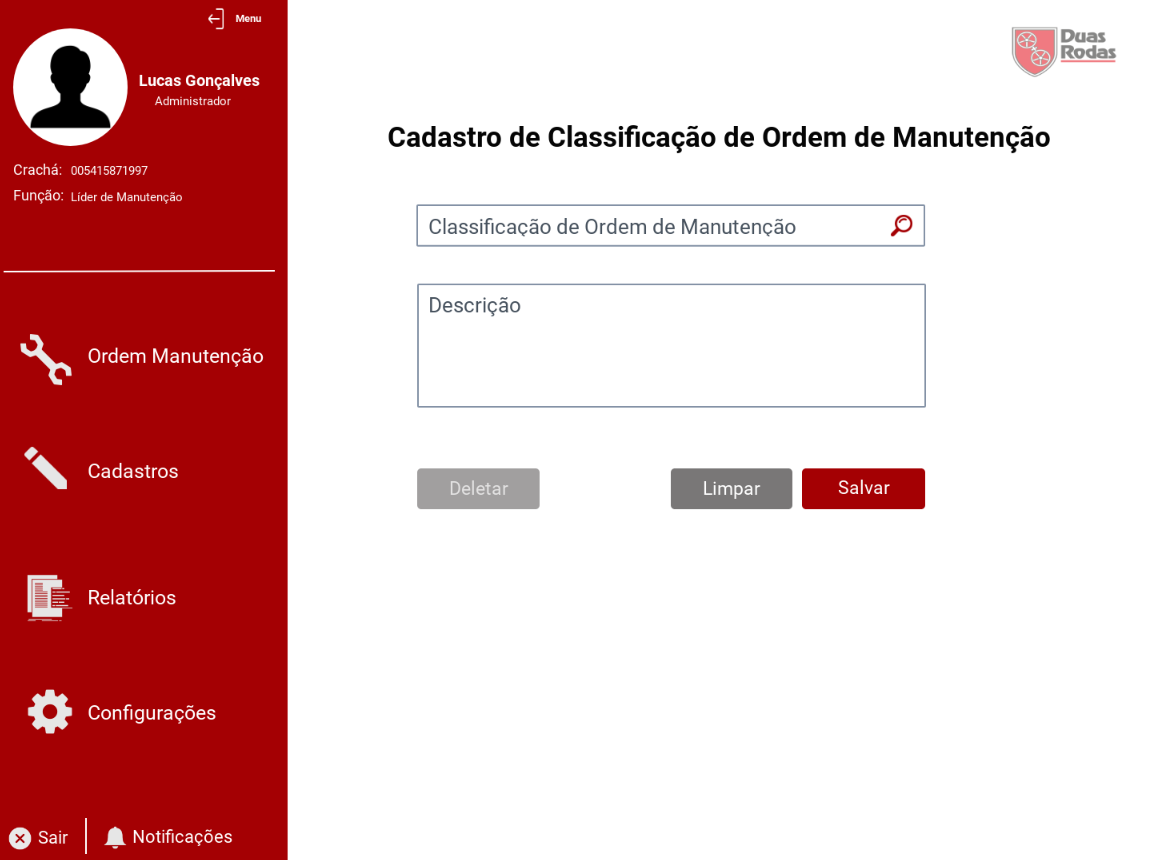
\includegraphics[scale=0.55]{./Figuras/web/cad-classificacao-om.png}
	\end{center}
	\legend{Fonte: Próprio Autor, 2019}
\end{figure}

Na tela \ref{web_cad-classificacao-om} será possível cadastrar as classificações da ordem de manutenção.

\newpage
\subsection{Cadastro de Tipo de Ordem de Manutenção}

\begin{figure}[htb]
	\caption{\label{web_cad-tipo-om}Cadastro de Tipo de Ordem de Manutenção}
	\begin{center}
		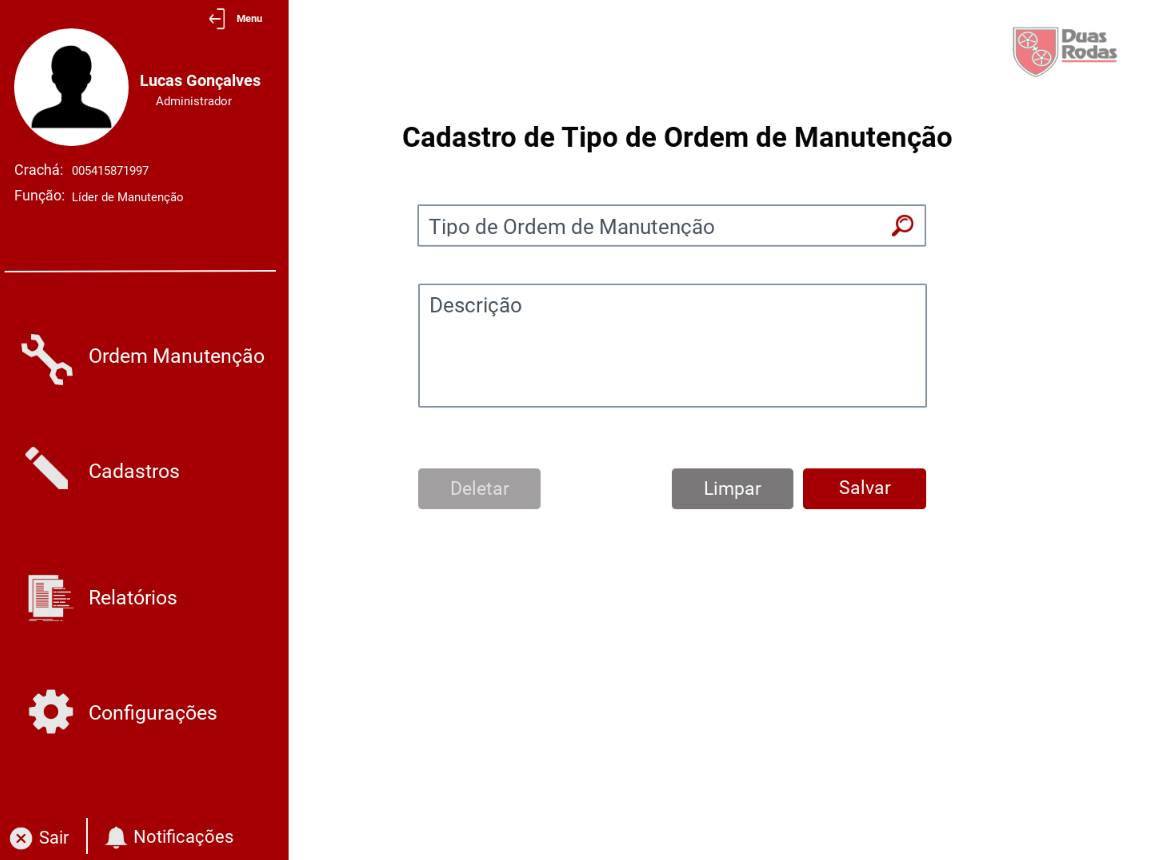
\includegraphics[scale=0.55]{./Figuras/web/cad-tipo-om.png}
	\end{center}
	\legend{Fonte: Próprio Autor, 2019}
\end{figure}

Na tela \ref{web_cad-tipo-om} será possível cadastrar os tipos de ordem de manutenção.

\newpage
\subsection{Cadastro de Centro de Custo}

\begin{figure}[htb]
	\caption{\label{web_cad-centro-custo}Cadastro de Centro de Custo}
	\begin{center}
		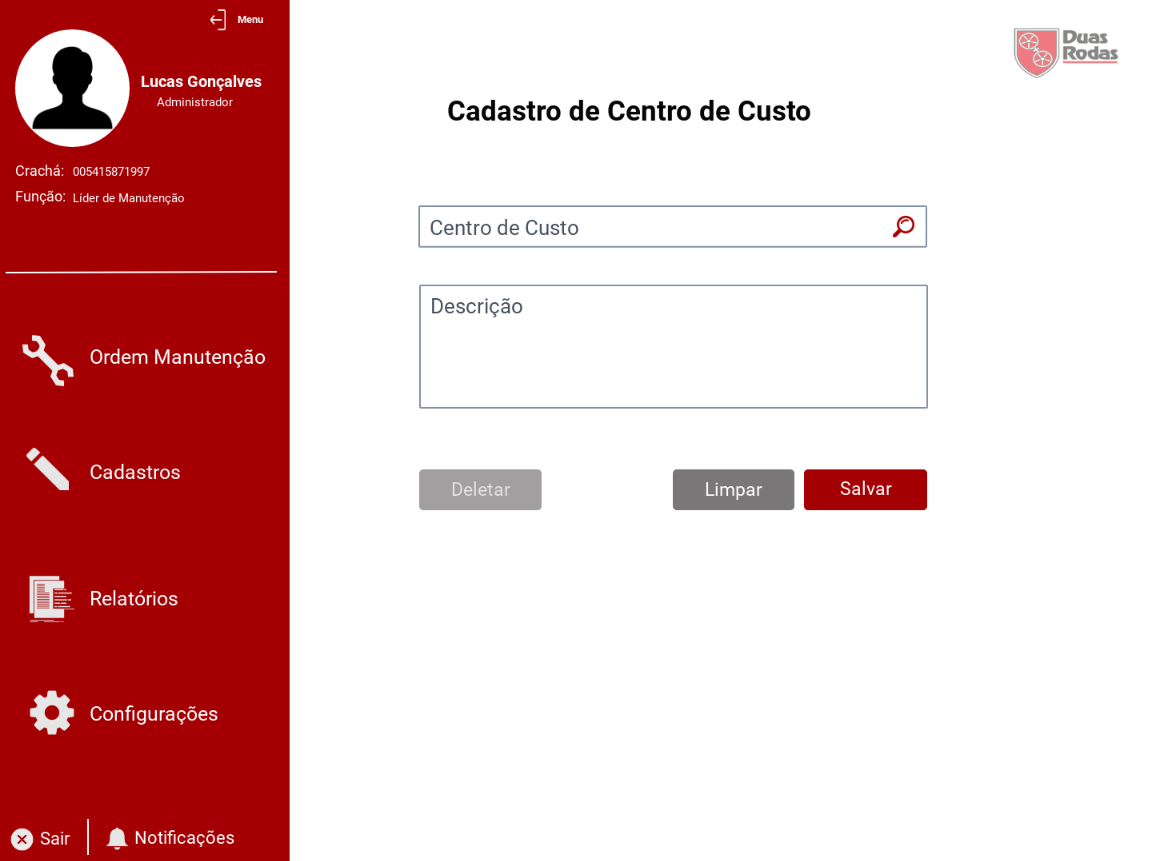
\includegraphics[scale=0.55]{./Figuras/web/cad-centro-custo.png}
	\end{center}
	\legend{Fonte: Próprio Autor, 2019}
\end{figure}

Na tela \ref{web_cad-centro-custo} é possível cadastrar centro de custo ao sistema.

\newpage
\subsection{Cadastro de Ordem de Manutenção}

\begin{figure}[htb]
	\caption{\label{web_cad-om}Cadastro de Ordem de Manutenção}
	\begin{center}
		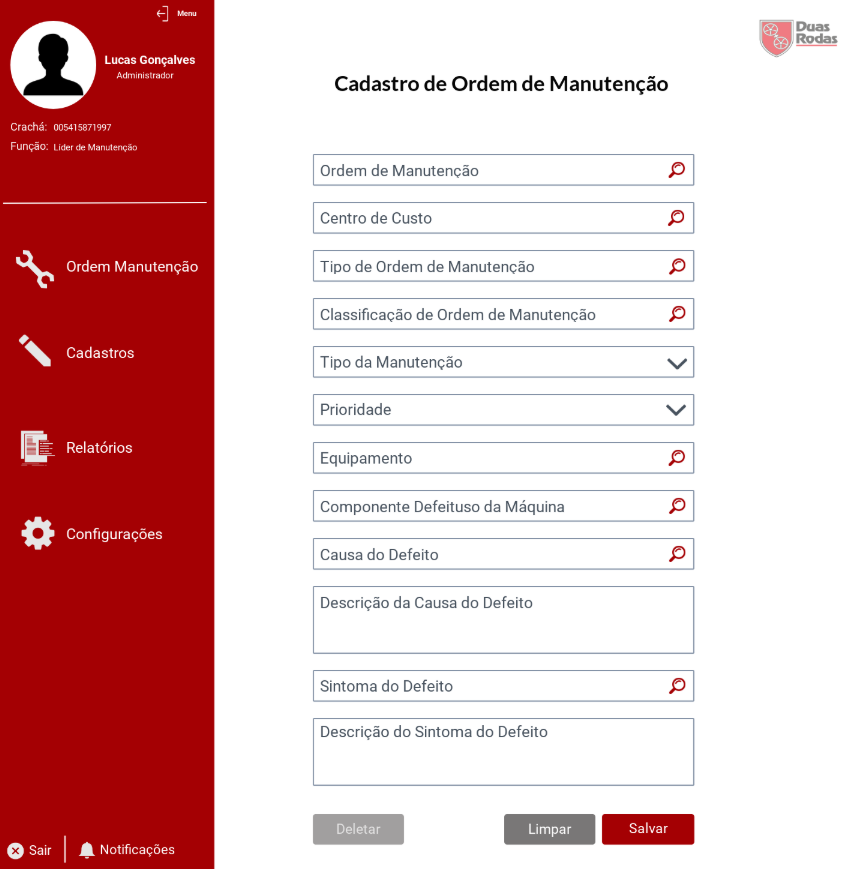
\includegraphics[scale=0.65]{./Figuras/web/cad-om.png}
	\end{center}
	\legend{Fonte: Próprio Autor, 2019}
\end{figure}

Na tela \ref{web_cad-om} é cadastrada e atualizada ordens de manutenção. Ela terá acesso às operações, componentes e assinaturas.

\newpage
\subsection{Cadastro de Parametrização de Status de Segurança}

\begin{figure}[htb]
	\caption{\label{web_param-status-seguranca}Cadastro de Parametrização de Status de Segurança}
	\begin{center}
		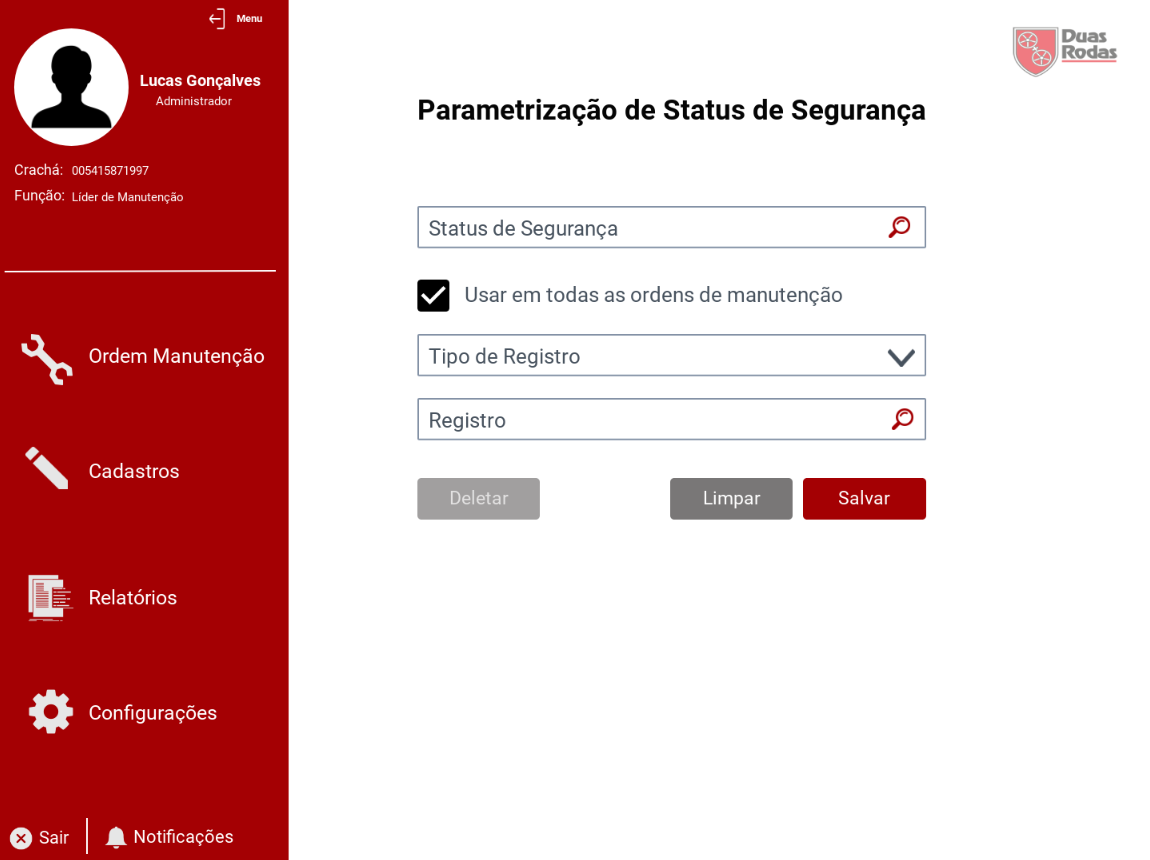
\includegraphics[scale=0.55]{./Figuras/web/param-status-seguranca.png}
	\end{center}
	\legend{Fonte: Próprio Autor, 2019}
\end{figure}

Na tela \ref{web_param-status-seguranca} é possível parametrizar quais serão a checklist de segurança que o manutentor terá de assinalar antes de iniciar uma manutenção.

\newpage
\subsection{Monitor de Ordem de Manutenção: Cards}

\begin{figure}[htb]
	\caption{\label{web_monitor-om-card}Monitor de Ordem de Manutenção: Cards}
	\begin{center}
		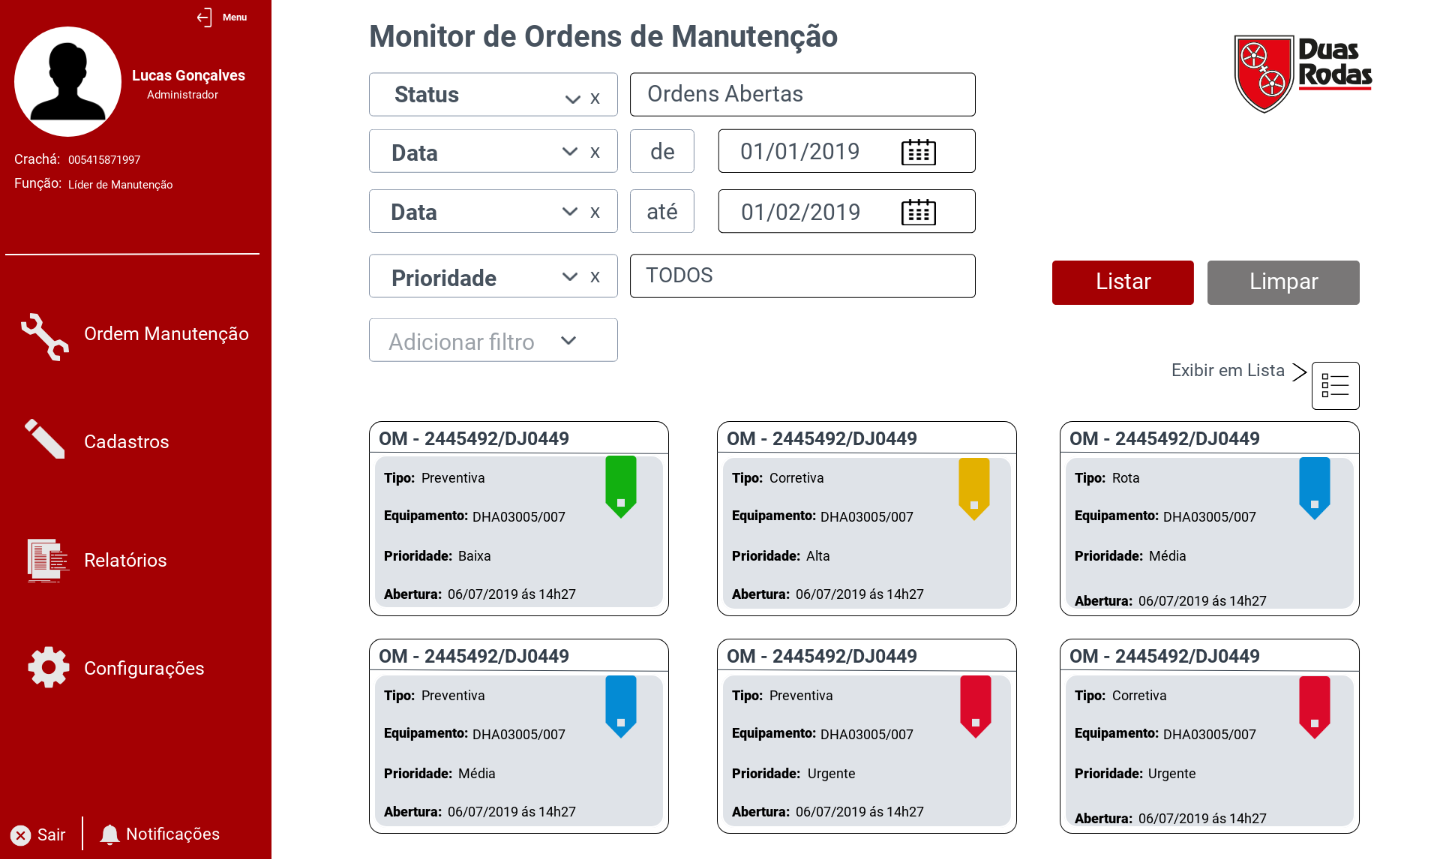
\includegraphics[scale=0.45]{./Figuras/web/monitor-om-card.png}
	\end{center}
	\legend{Fonte: Próprio Autor, 2019}
\end{figure}

A tela \ref{web_monitor-om-card} permite a consulta rápida e dinâmica das ordens de manutenção. Nela você pode aplicar os filtros de acordo com as \newline necessidades e será listada em forma de cartões, eles darão acesso à uma tela de detalhamento de ordem de manutenção.

\newpage
\subsection{Monitor de Ordem de Manutenção: Listas}

\begin{figure}[htb]
	\caption{\label{web_monitor-om-lista}Monitor de Ordem de Manutenção: Listas}
	\begin{center}
		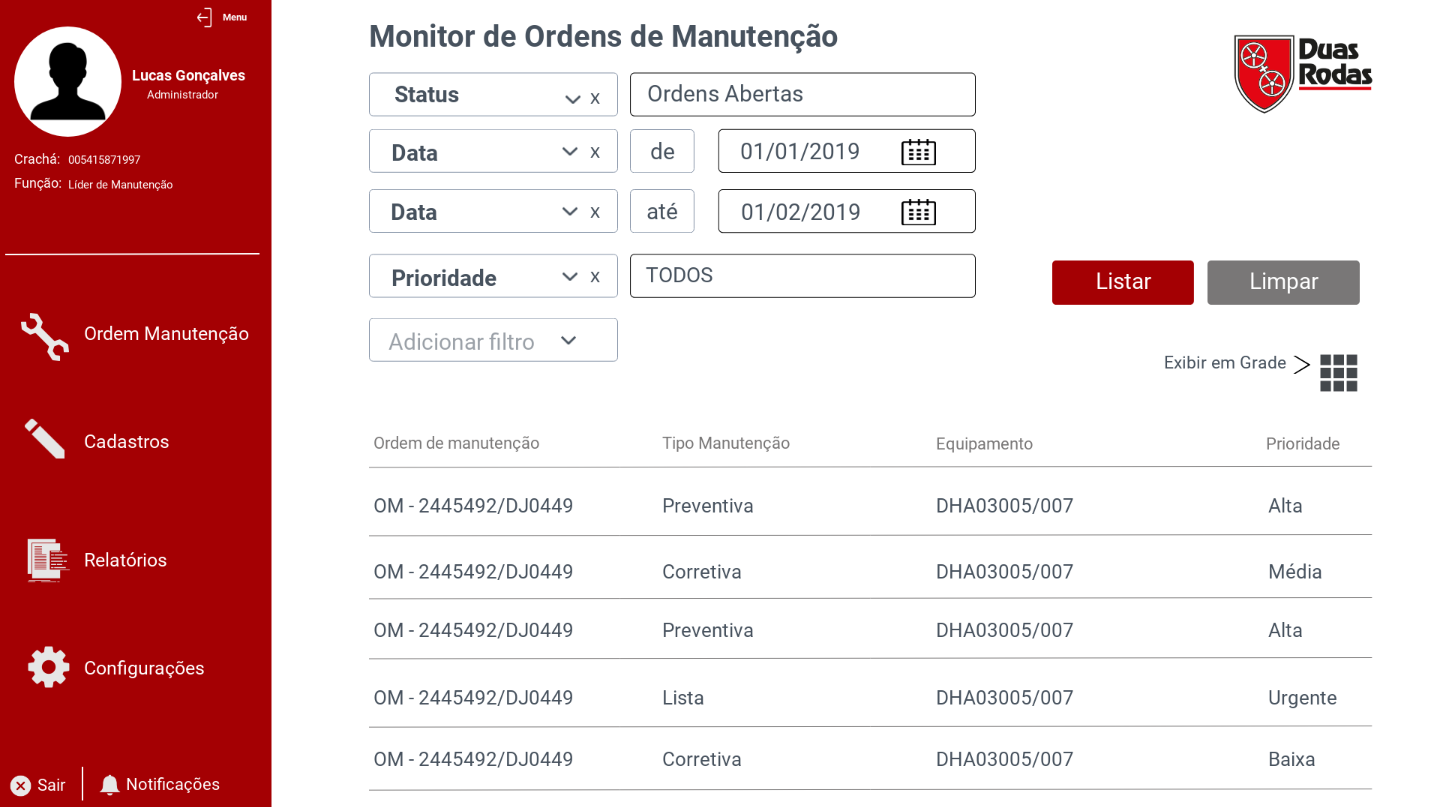
\includegraphics[scale=0.45]{./Figuras/web/monitor-om-lista.png}
	\end{center}
	\legend{Fonte: Próprio Autor, 2019}
\end{figure}

A tela \ref{web_monitor-om-lista} permite a consulta rápida e dinâmica das ordens de manutenção. Nela você pode aplicar os filtros de acordo com as \newline necessidades e será listada em forma de listas, eles darão acesso à uma tela de detalhamento de ordem de manutenção.

\newpage
\subsection{Ordem de Manutenção}

\begin{figure}[htb]
	\caption{\label{web_om-capa}Ordem de Manutenção}
	\begin{center}
		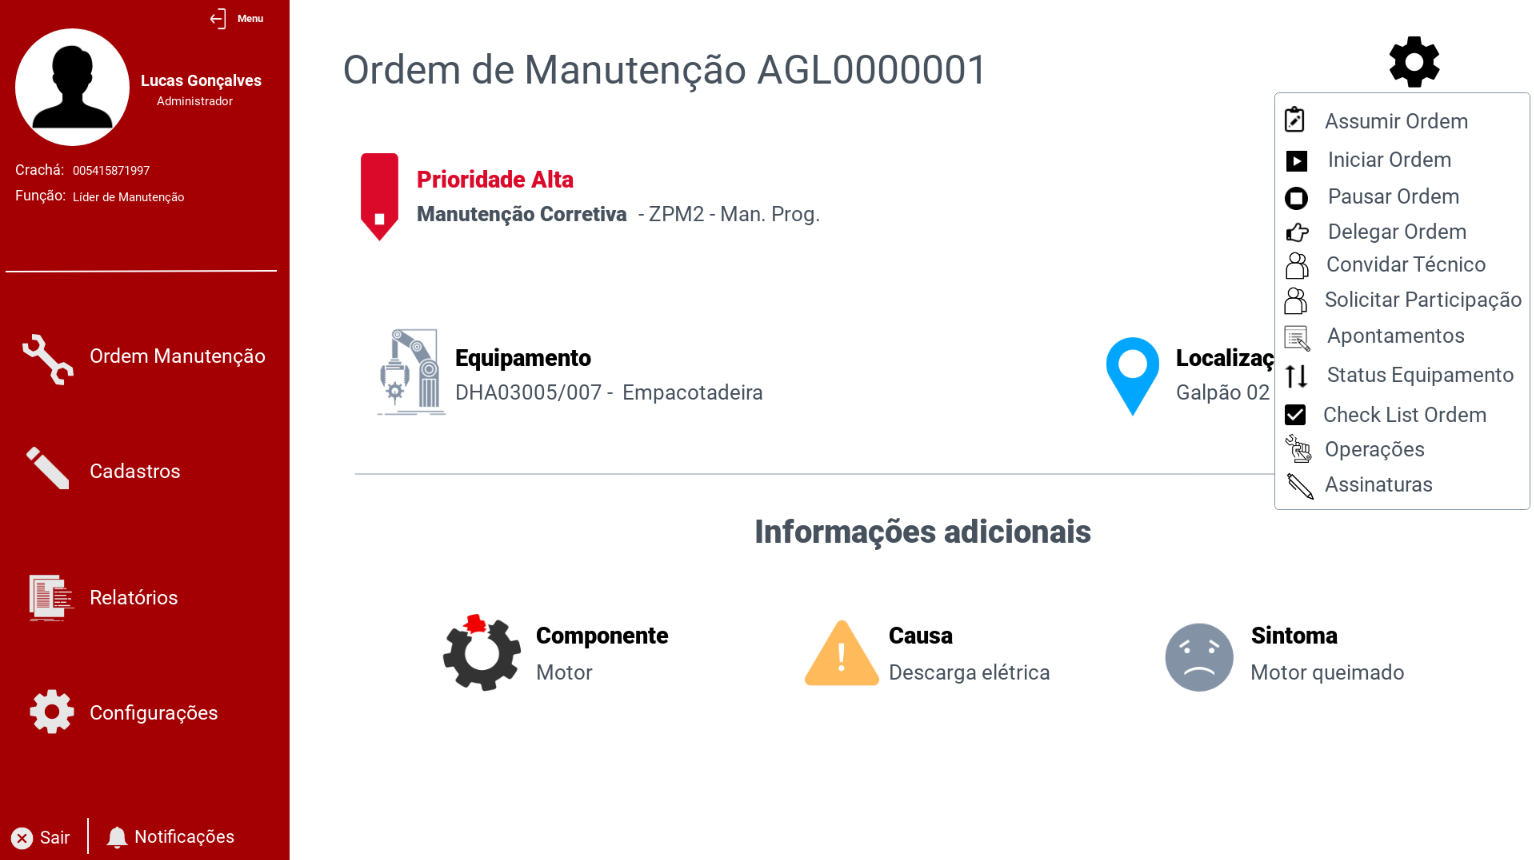
\includegraphics[scale=0.40]{./Figuras/web/om-capa.png}
	\end{center}
	\legend{Fonte: Próprio Autor, 2019}
\end{figure}

Na tela \ref{web_om-capa} será possível acompanhar o andamento de uma ordem de manutenção de lista, ver informações referente à ordem e executar ações nela, como alterar status, adicionar operações e realizar assinaturas.

\newpage
\subsection{Checklist de Segurança}

\begin{figure}[htb]
	\caption{\label{web_check-list}Checklist de Segurança}
	\begin{center}
		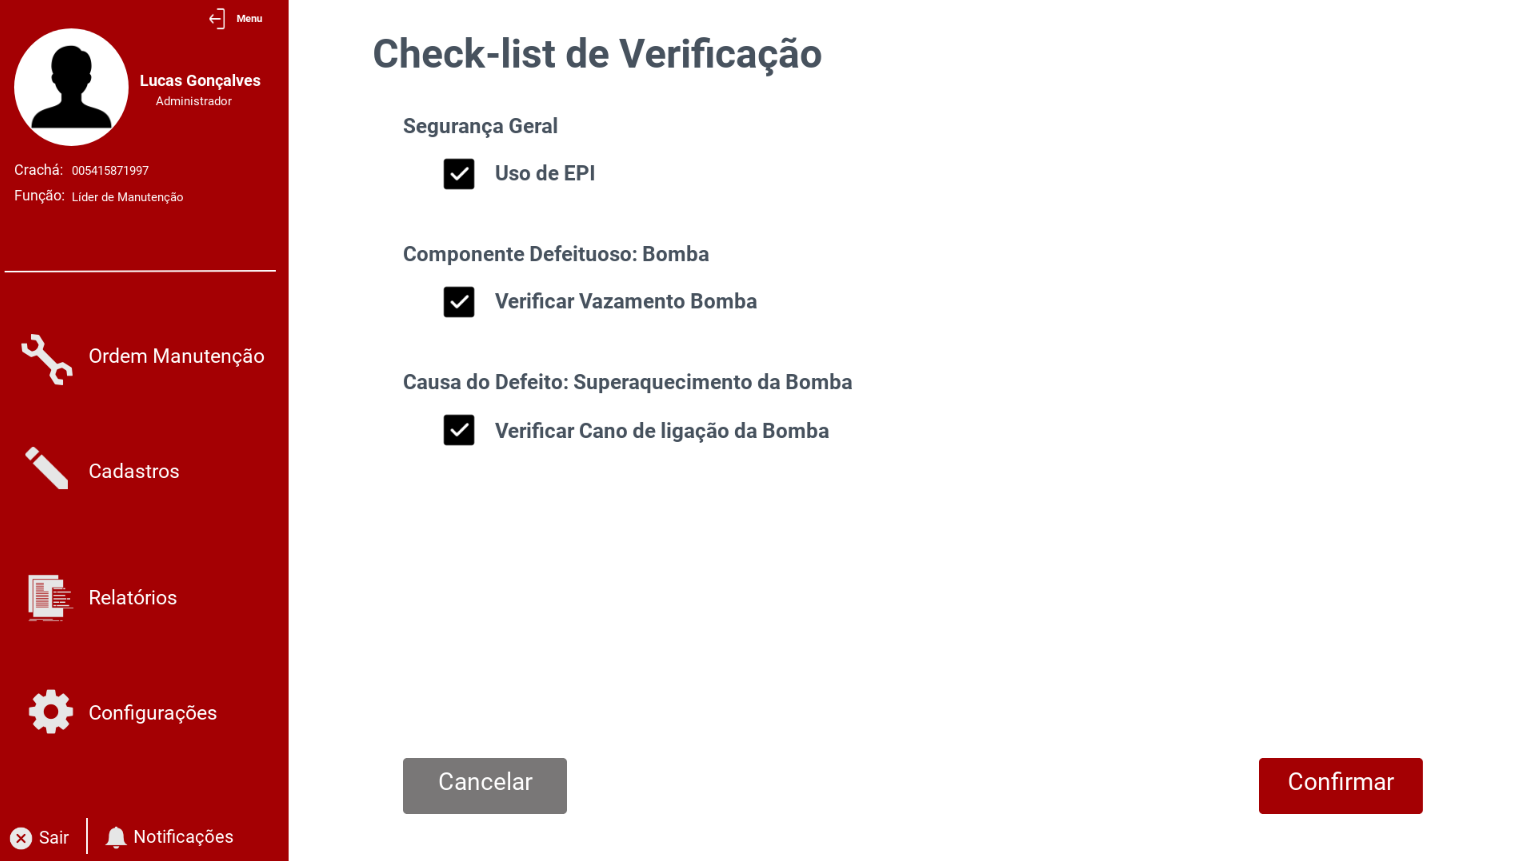
\includegraphics[scale=0.40]{./Figuras/web/check-list.png}
	\end{center}
	\legend{Fonte: Próprio Autor, 2019}
\end{figure}

Na tela \ref{web_check-list} o manutentor irá marcar a lista de segurança antes de iniciar a ordem de manutenção.

\newpage
\subsection{Operações da Ordem de Manutenção}

\begin{figure}[htb]
	\caption{\label{web_om-operacoes}Operações da Ordem de Manutenção}
	\begin{center}
		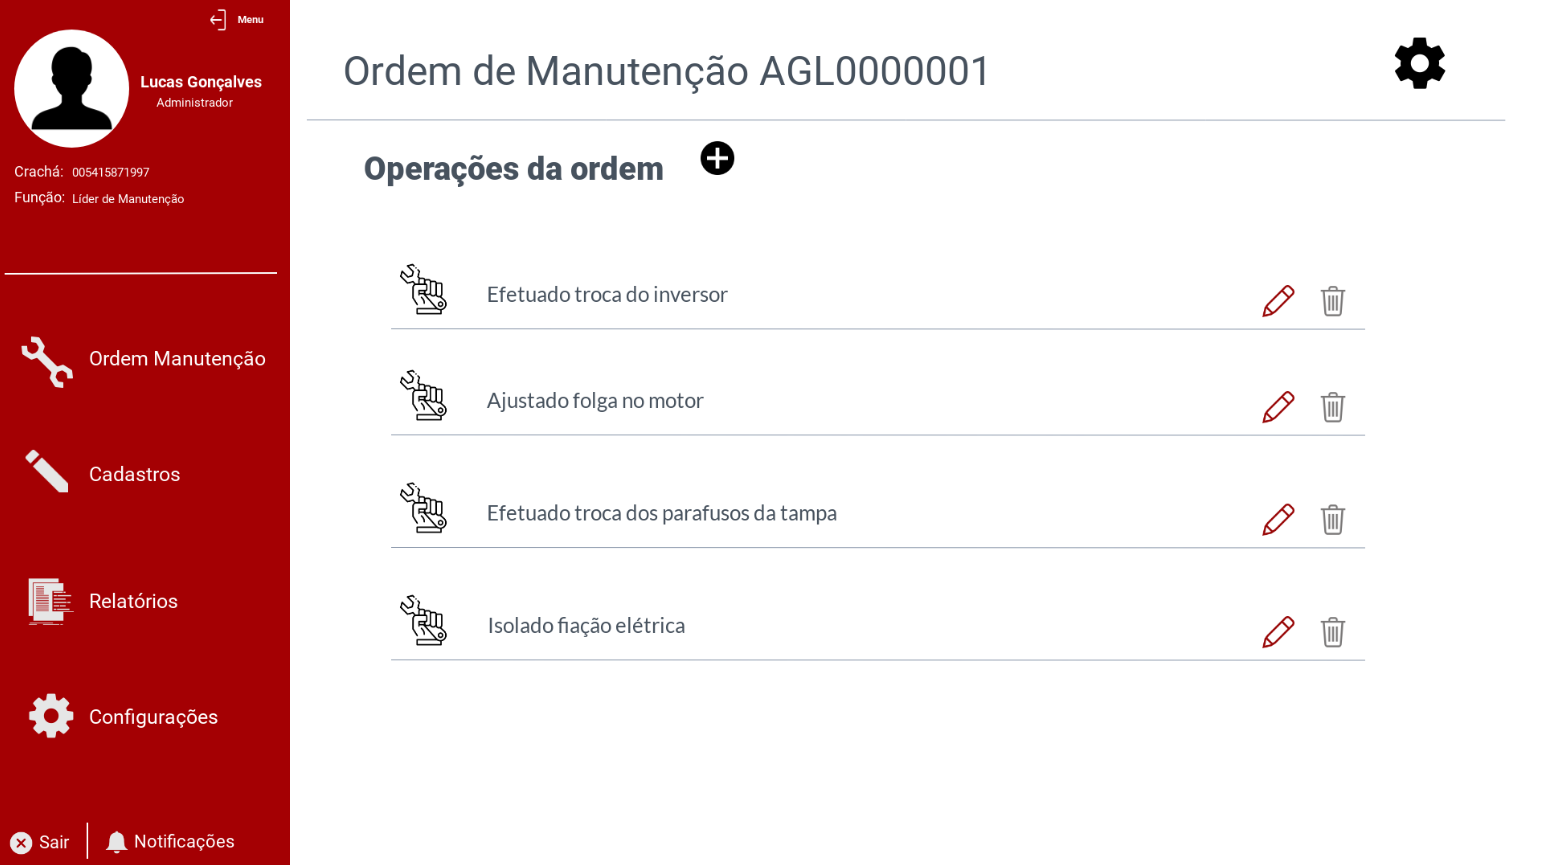
\includegraphics[scale=0.40]{./Figuras/web/om-operacoes.png}
	\end{center}
	\legend{Fonte: Próprio Autor, 2019}
\end{figure}

Na tela \ref{web_om-operacoes} é possível verificar todas as operações pré cadastradas para a OM e cadastrar novas operações conforme necessidade para o andamento da OM.

\newpage
\subsection{Ordem de Manutenção: Lista}

\begin{figure}[htb]
	\caption{\label{web_om-lista}Ordem de Manutenção: Lista}
	\begin{center}
		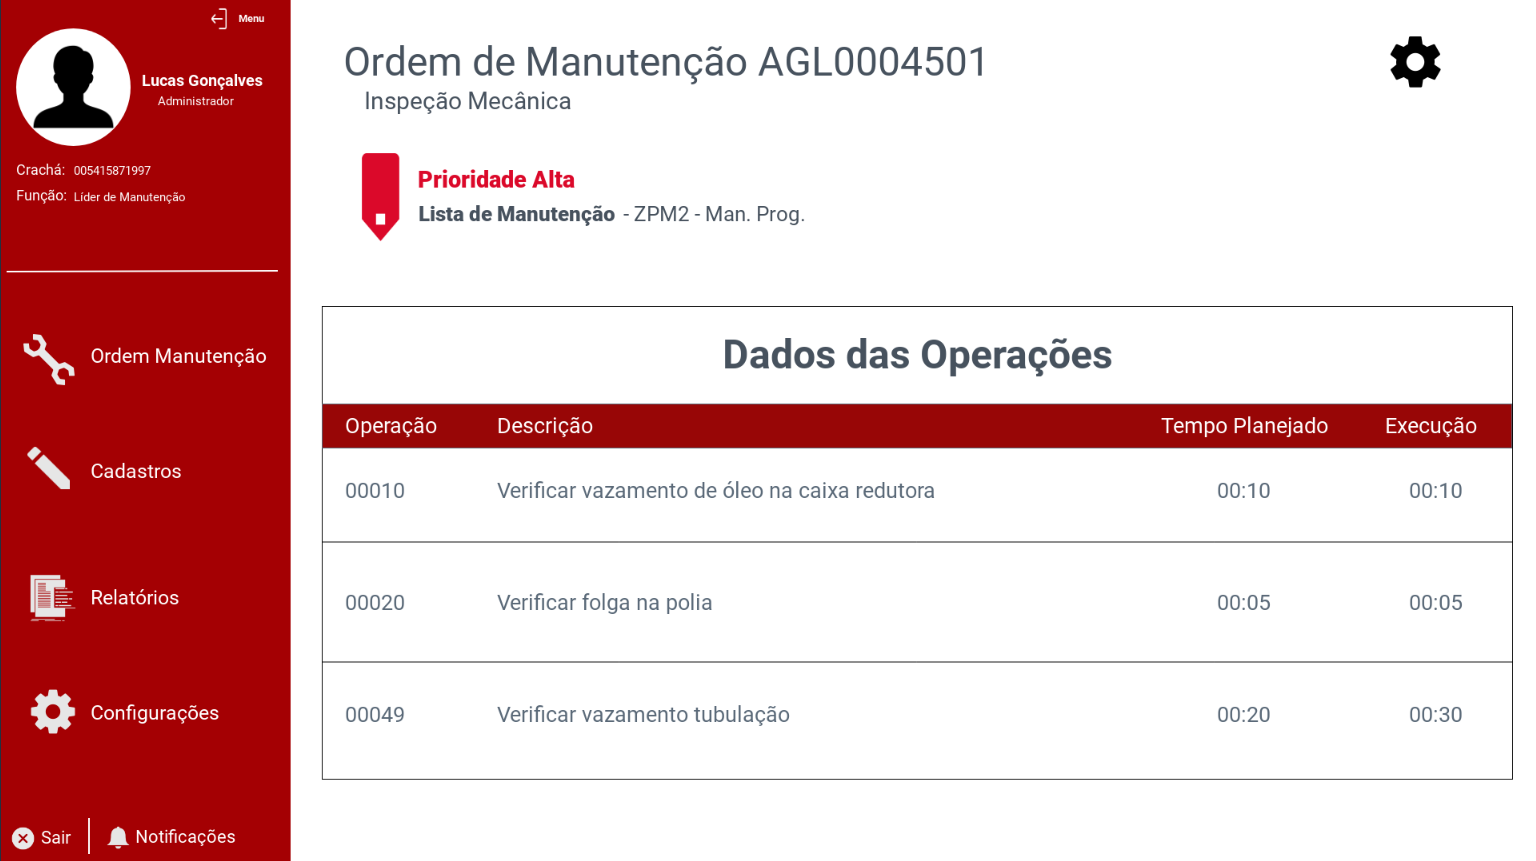
\includegraphics[scale=0.40]{./Figuras/web/om-lista.png}
	\end{center}
	\legend{Fonte: Próprio Autor, 2019}
\end{figure}

Na tela \ref{web_om-lista} será possível acompanhar o andamento de uma ordem de manutenção de lista, ver informações referente à ordem e executar ações nela, como alterar status, adicionar operações e realizar assinaturas.

\newpage
\subsection{Equipamentos da Ordem de Manutenção: Lista}

\begin{figure}[htb]
	\caption{\label{web_om-lista-equipamentos}Equipamentos da Ordem de Manutenção: Lista}
	\begin{center}
		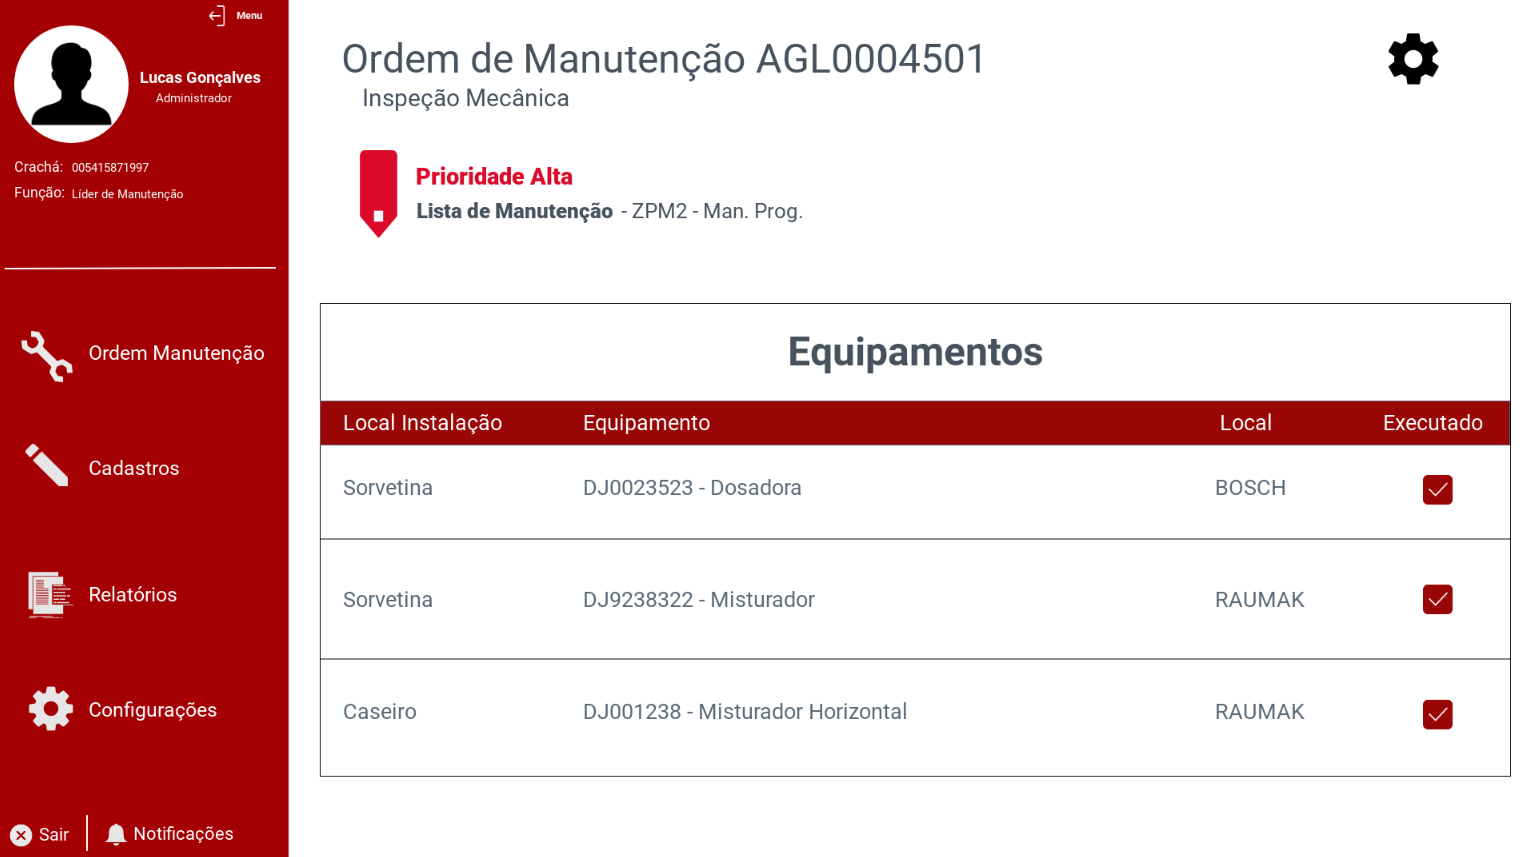
\includegraphics[scale=0.40]{./Figuras/web/om-lista-equipamentos.png}
	\end{center}
	\legend{Fonte: Próprio Autor, 2019}
\end{figure}

Na tela \ref{web_om-lista-equipamentos} será possível acompanhar os equipamentos que terão de ser inspecionados pelo manutentor e o mesmo marcar se executou ou não.

\newpage
\subsection{Ordem de Manutenção: Rota}

\begin{figure}[htb]
	\caption{\label{web_om-rota}Ordem de Manutenção: Rota}
	\begin{center}
		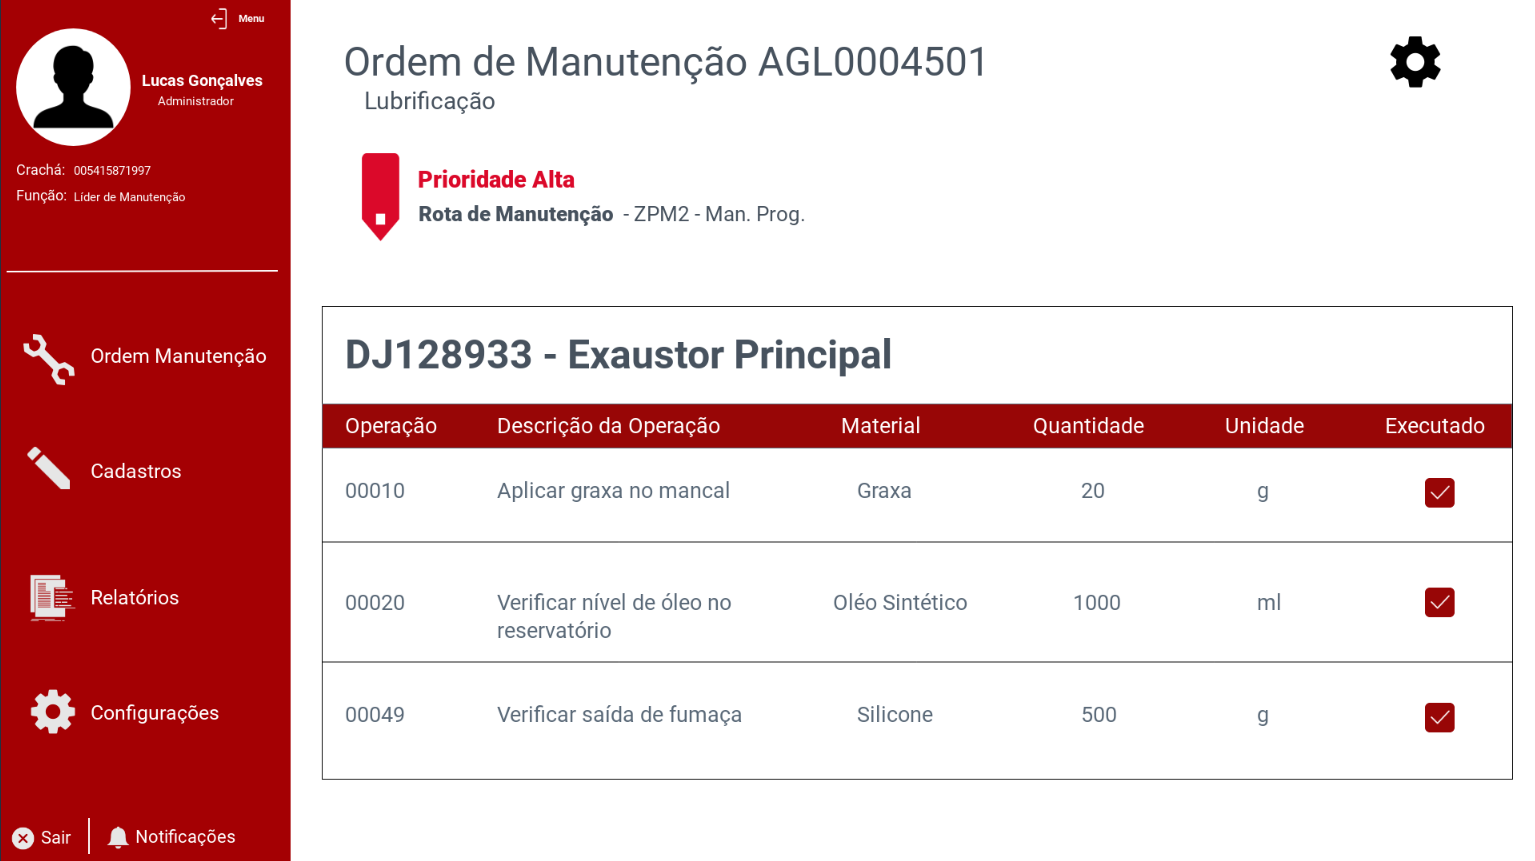
\includegraphics[scale=0.40]{./Figuras/web/om-rota.png}
	\end{center}
	\legend{Fonte: Próprio Autor, 2019}
\end{figure}

Na tela \ref{web_om-rota} será possível acompanhar o andamento de uma ordem de manutenção de lista, ver informações referente à ordem e executar ações nela, como alterar status, adicionar operações e realizar assinaturas.

\newpage
\subsection{Convidar ou Delegar Ordem de Manutenção}

\begin{figure}[htb]
	\caption{\label{web_om-convidar-delegar}Convidar ou Delegar Ordem de Manutenção}
	\begin{center}
		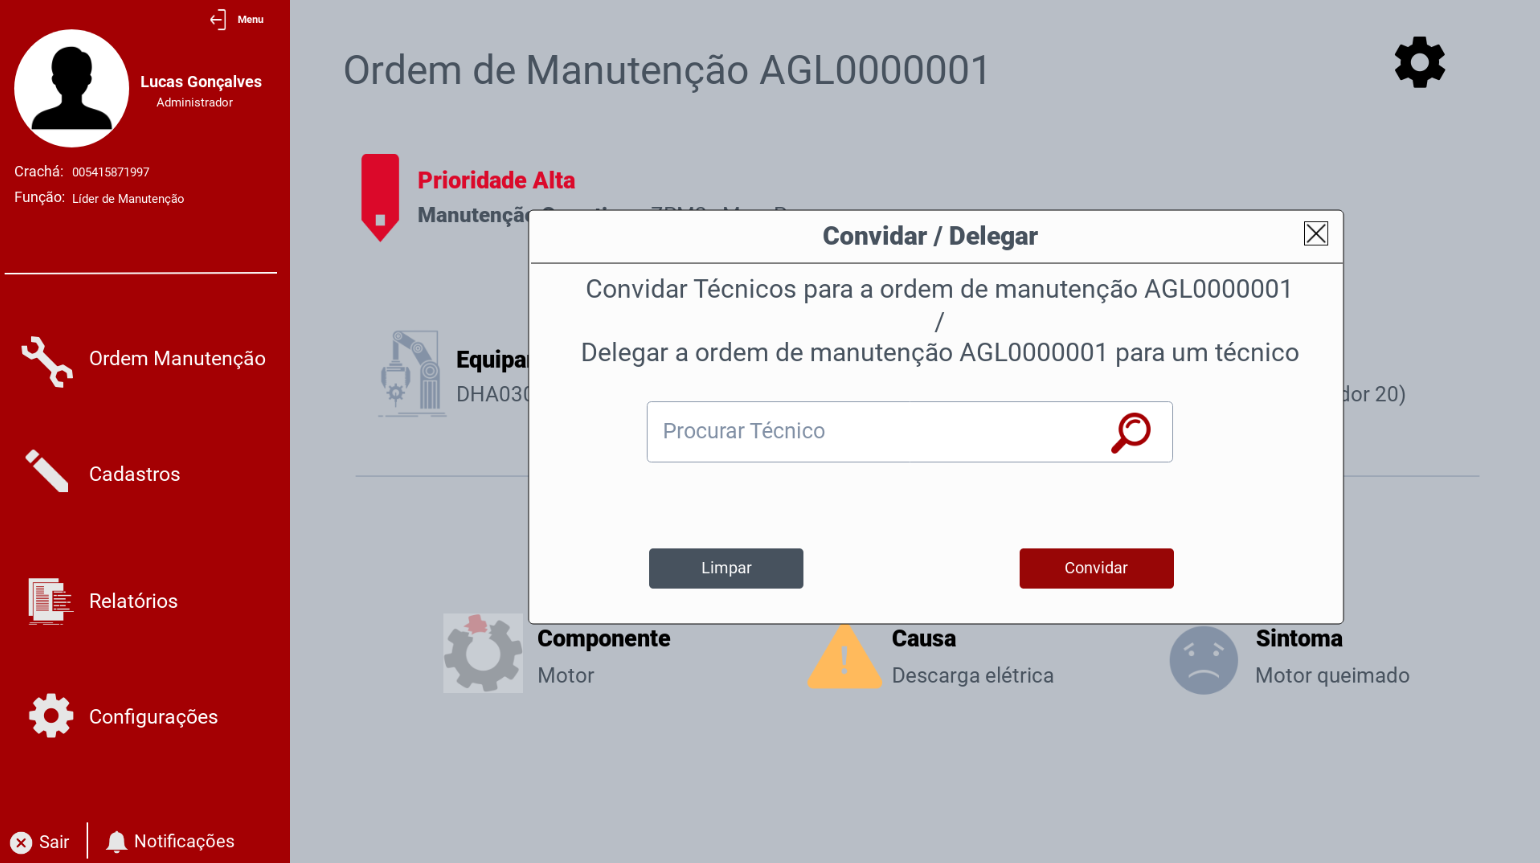
\includegraphics[scale=0.40]{./Figuras/web/om-convidar-delegar.png}
	\end{center}
	\legend{Fonte: Próprio Autor, 2019}
\end{figure}

Na tela \ref{web_om-convidar-delegar} será possível convidar técnicos para se juntarem a ordem de manutenção ou delegar a ordem de manutenção a outro manutentor. Ação só permitida àqueles que são responsáveis pela ordem de manutenção, ou seja, os que assumiram ela.

\newpage
\subsection{Apontamentos}

\begin{figure}[htb]
	\caption{\label{web_om-apontamentos}Apontamentos da Ordem de Manutenção}
	\begin{center}
		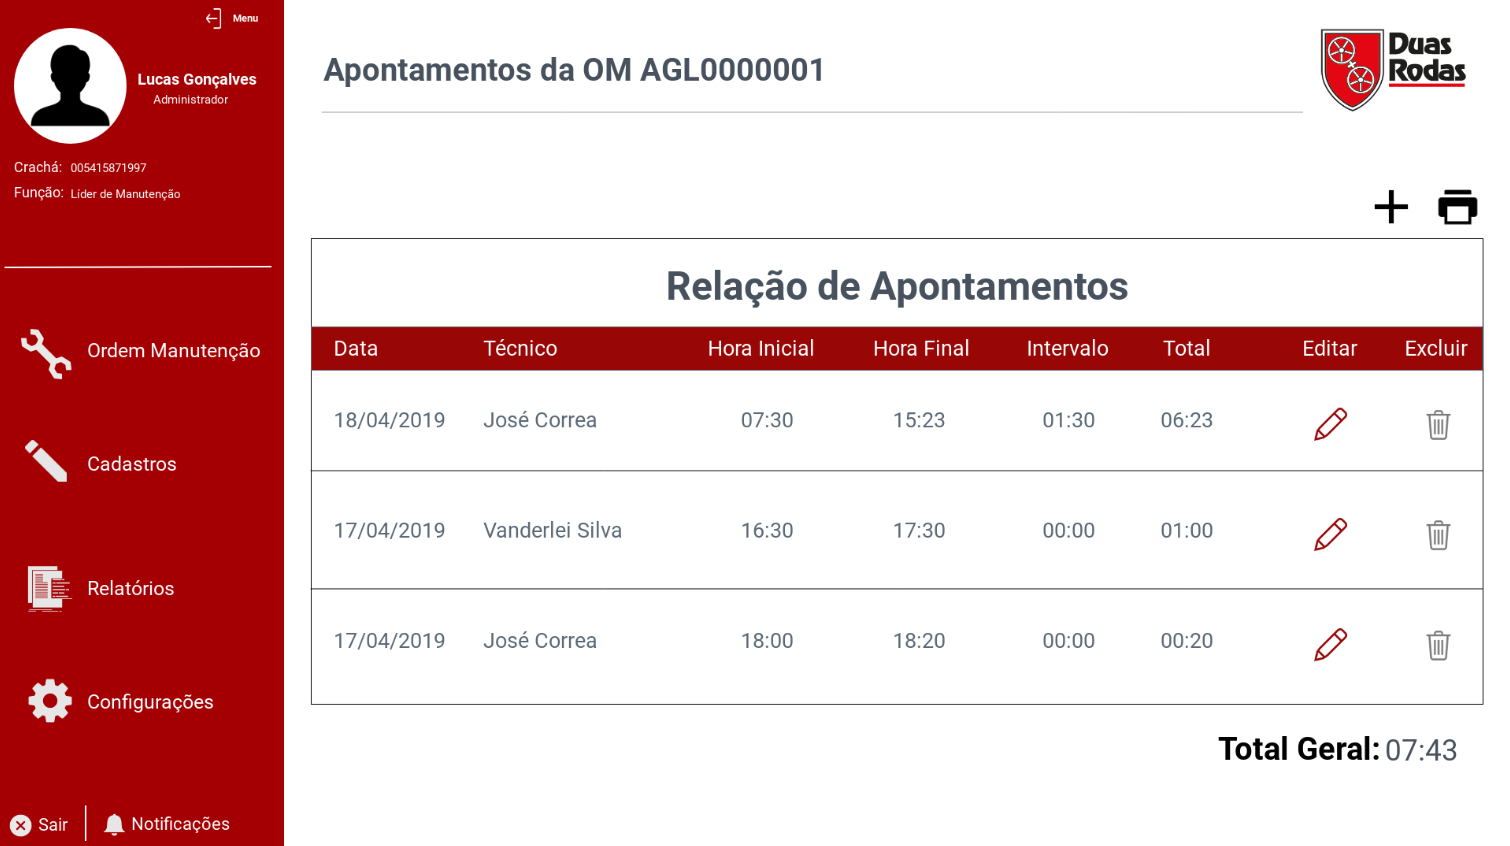
\includegraphics[scale=0.40]{./Figuras/web/om-apontamentos.png}
	\end{center}
	\legend{Fonte: Próprio Autor, 2019}
\end{figure}

Na tela \ref{web_om-apontamentos} será possível visualizar todos os apontamentos que existem em uma ordem, atualizá-las, excluí-las ou adicionar novos apontamentos.

\newpage
\subsection{Adicionar Apontamentos}

\begin{figure}[htb]
	\caption{\label{web_om-add-apontamento}Adicionar Apontamentos na Ordem de Manutenção}
	\begin{center}
		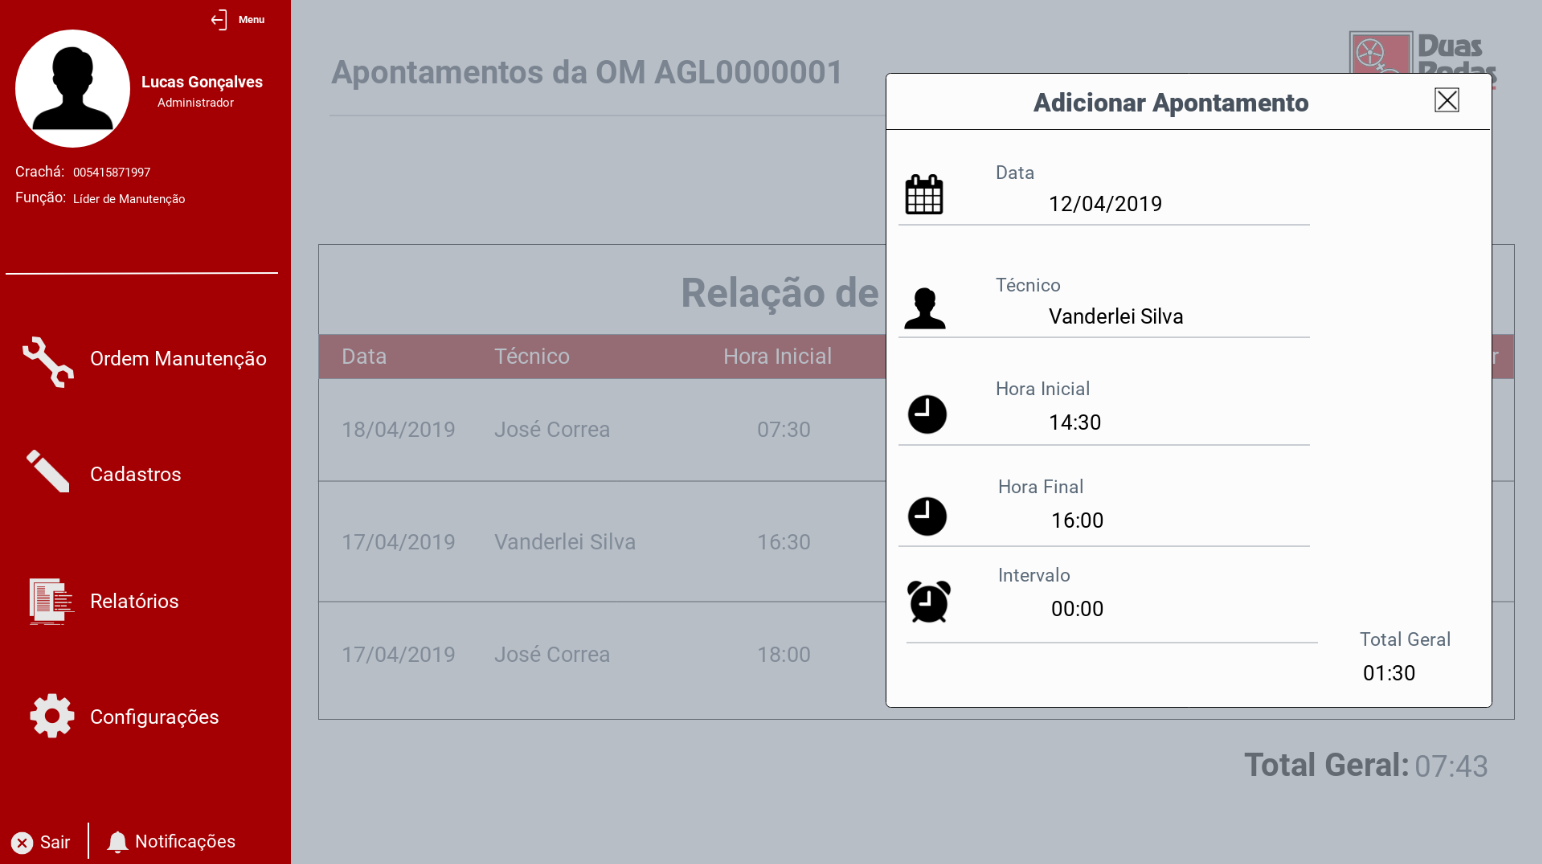
\includegraphics[scale=0.40]{./Figuras/web/om-add-apontamento.png}
	\end{center}
	\legend{Fonte: Próprio Autor, 2019}
\end{figure}

Na tela \ref{web_om-add-apontamento} será possível adicionar novos apontamentos a ordem de manutenção.

\newpage
\subsection{Motivo da Exclusão do Apontamento da Ordem de Manutenção}

\begin{figure}[htb]
	\caption{\label{web_om-excluir-apontamento-motivo}Motivo da Exclusão do Apontamento da Ordem de Manutenção}
	\begin{center}
		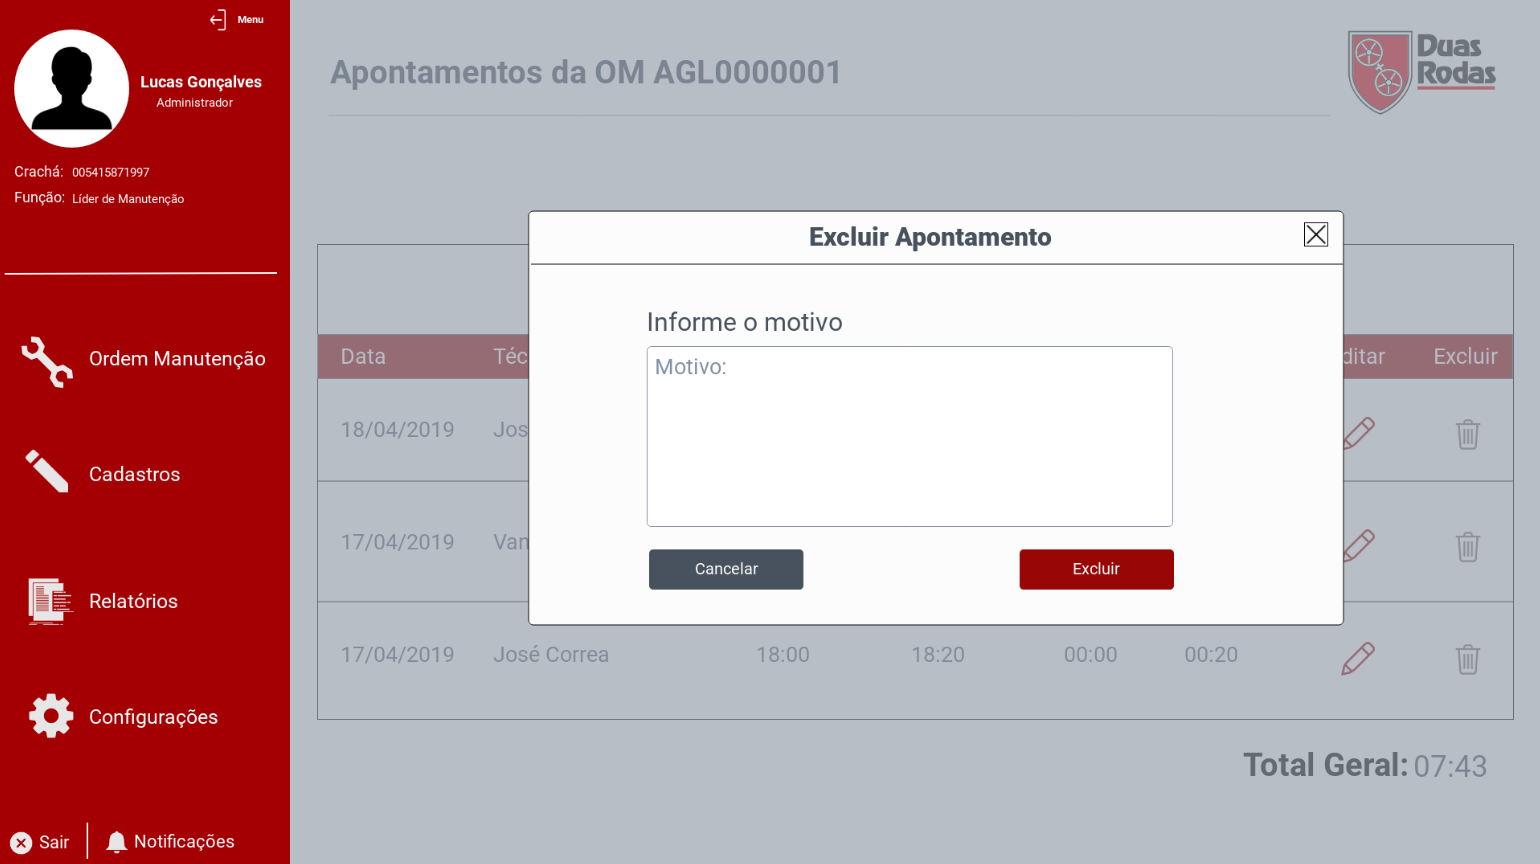
\includegraphics[scale=0.40]{./Figuras/web/om-excluir-apontamento-motivo.png}
	\end{center}
	\legend{Fonte: Próprio Autor, 2019}
\end{figure}

Na tela \ref{web_om-excluir-apontamento-motivo} o operador terá de informar o motivo pela exclusão do apontamento da ordem de manutenção.

\newpage
\subsection{Assinatura Digital}

\begin{figure}[htb]
	\caption{\label{web_om-assinatura}Assinatura Digital}
	\begin{center}
		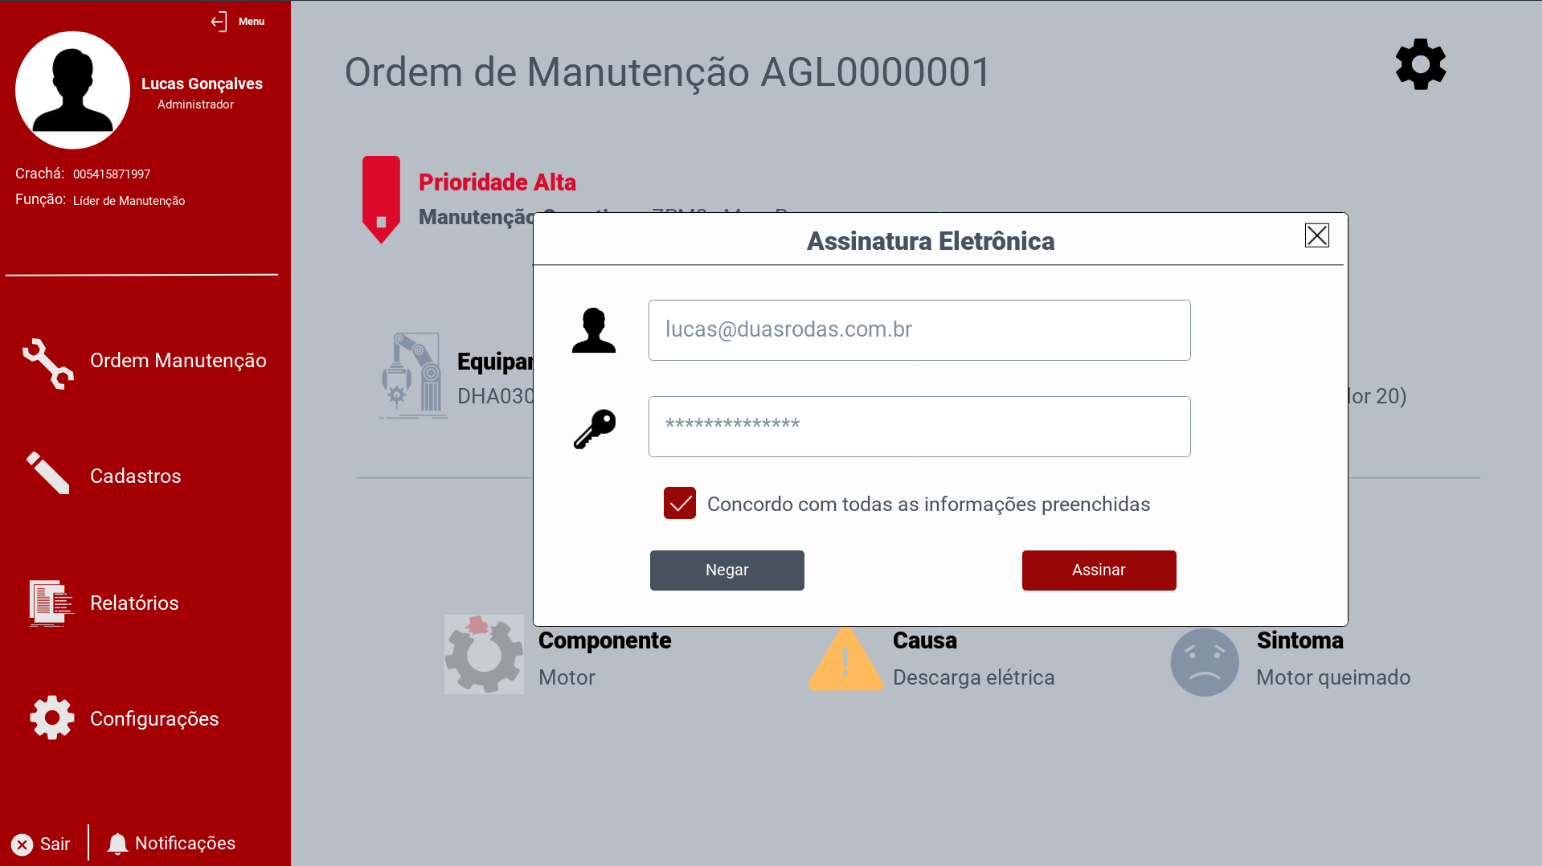
\includegraphics[scale=0.40]{./Figuras/web/om-assinatura.png}
	\end{center}
	\legend{Fonte: Próprio Autor, 2019}
\end{figure}

Na tela \ref{web_om-assinatura} será possível assinar a ordem digitalmente. Para tanto, será cobrado as credenciais do operador.

\newpage
\subsection{Central de Notificações}

\begin{figure}[htb]
	\caption{\label{web_central-notificacoes}Central de Notificações}
	\begin{center}
		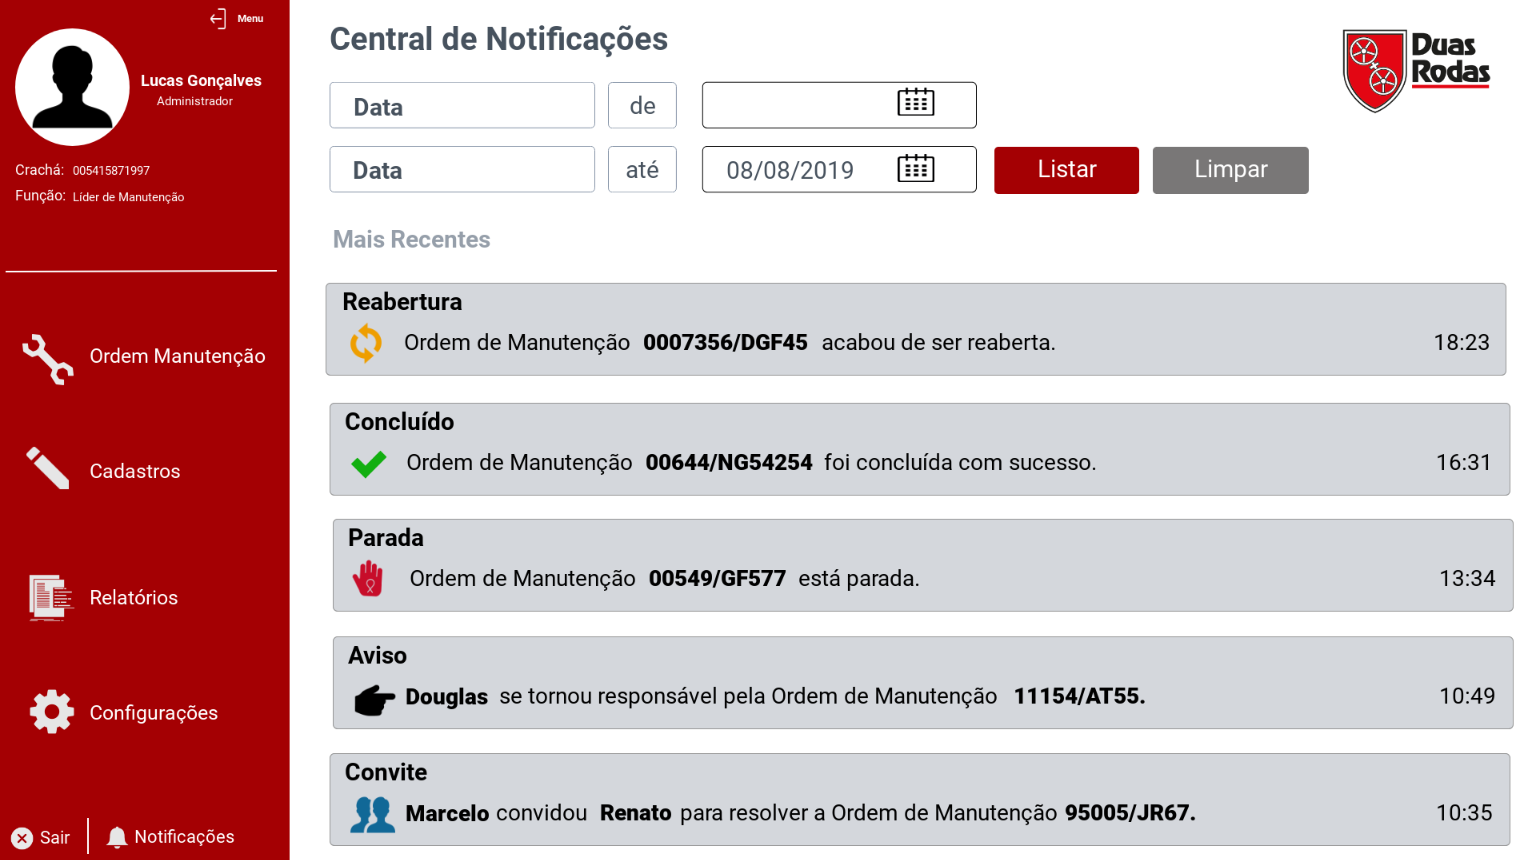
\includegraphics[scale=0.40]{./Figuras/web/central-notificacoes.png}
	\end{center}
	\legend{Fonte: Próprio Autor, 2019}
\end{figure}

Na tela \ref{web_central-notificacoes} é possível verificar notificações do usuário autenticado.

\newpage
\section{Aplicação Mobile}
A aplicação Mobile é um ponto estratégico do produto, pois sua mobilidade permite com que os técnicos possam atuar na manutenção e realizar anotações e apontamentos no sistema através de um smartphone ou tablet.

\subsection{Login}

\begin{figure}[htb]
	\caption{\label{mobile_login}Login}
	\begin{center}
		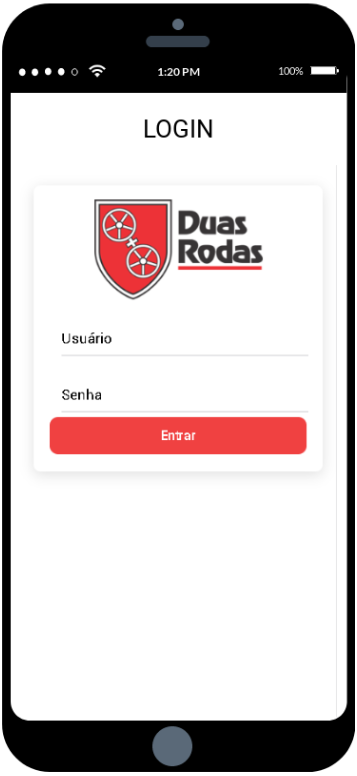
\includegraphics[scale=0.80]{./Figuras/mobile/login.png}
	\end{center}
	\legend{Fonte: Próprio Autor, 2019}
\end{figure}

A tela \ref{mobile_login} será a página responsável por autenticar o usuário e garantir a segurança do sistema.

\newpage
\subsection{Menu}

\begin{figure}[htb]
	\caption{\label{mobile_menu}Menu}
	\begin{center}
		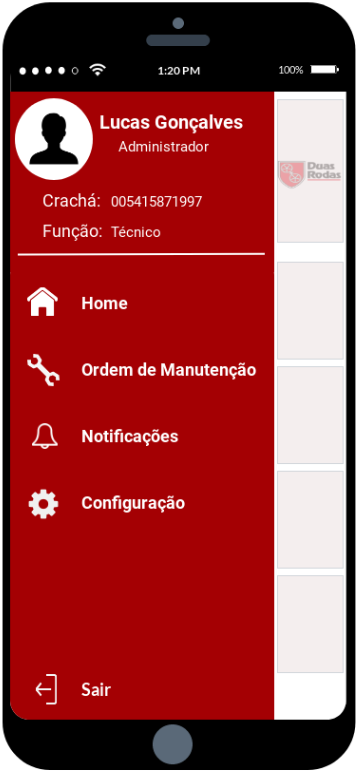
\includegraphics[scale=0.80]{./Figuras/mobile/menu.png}
	\end{center}
	\legend{Fonte: Próprio Autor, 2019}
\end{figure}

A figura \ref{mobile_menu} demonstra o menu lateral do aplicativo, identificando o usuário autenticado e um menu de acesso rápido às principais telas do sistema.

\newpage
\subsection{Monitor}

\begin{figure}[htb]
	\caption{\label{mobile_monitor}Monitor}
	\begin{center}
		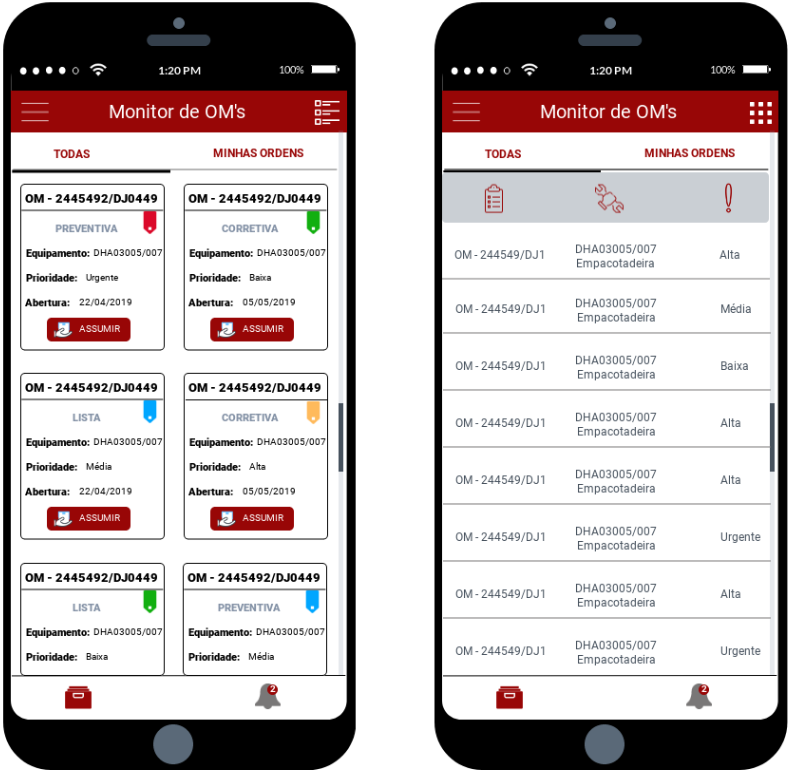
\includegraphics[scale=0.75]{./Figuras/mobile/monitor.png}
	\end{center}
	\legend{Fonte: Próprio Autor, 2019}
\end{figure}

Na figura \ref{mobile_monitor} é possível verificar o monitor do manutentor. Nesse monitor, o manutentor consegue rapidamente visualizar as OMs pendentes e seus respectivos status através das bandeiras indicadas no card. As  vermelhas indicam que a OM tem uma prioridade emergente, as amarelas têm prioridade alta, as azuis têm prioridade média e as verdes possuem uma prioridade baixa.

\newpage
\subsection{Central de Notificações}

\begin{figure}[htb]
	\caption{\label{mobile_notificacao}Notificações}
	\begin{center}
		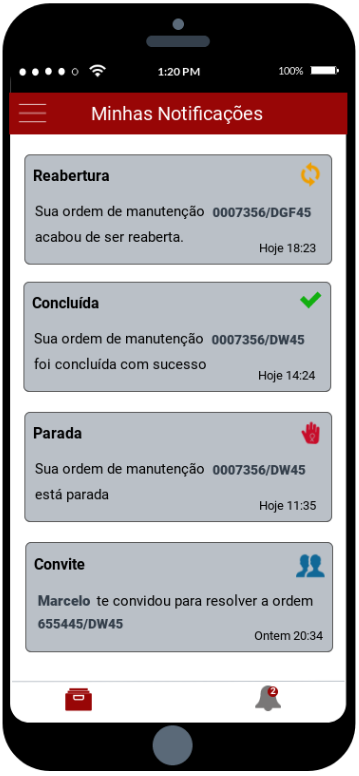
\includegraphics[scale=0.80]{./Figuras/mobile/notificacao.png}
	\end{center}
	\legend{Fonte: Próprio Autor, 2019}
\end{figure}

Na tela \ref{mobile_notificacao} é possível verificar notificações do usuário autenticado no sistema.

\newpage
\subsection{Ordem de Manutenção}

\begin{figure}[htb]
	\caption{\label{mobile_om}Ordem de Manutenção}
	\begin{center}
		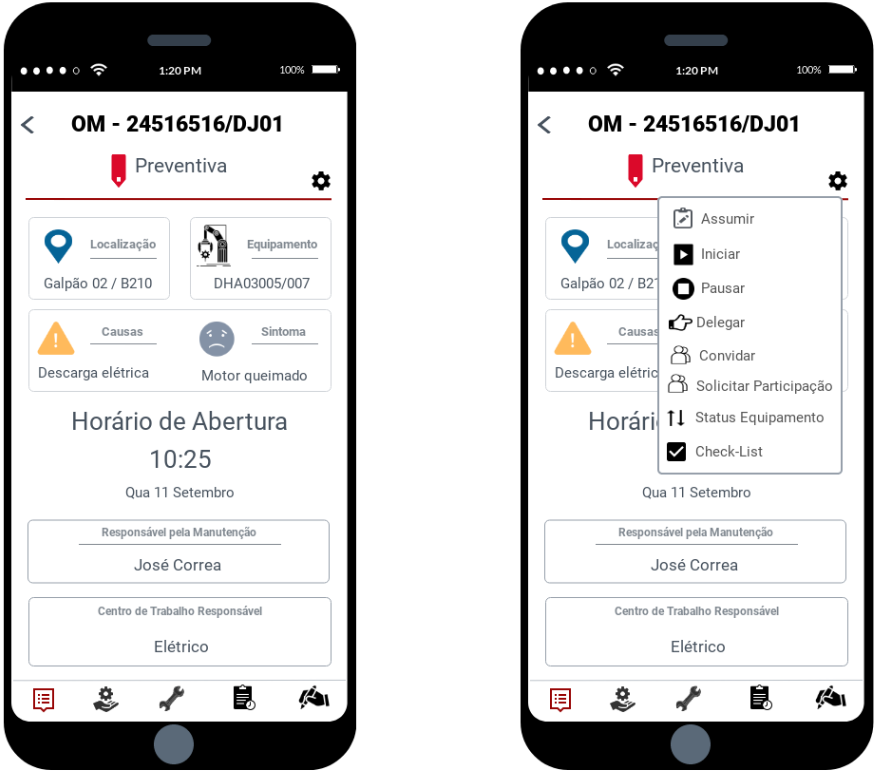
\includegraphics[scale=0.70]{./Figuras/mobile/om.png}
	\end{center}
	\legend{Fonte: Próprio Autor, 2019}
\end{figure}

Na tela \ref{mobile_om} será possível acompanhar o andamento de uma ordem de manutenção preventiva e corretiva, ver informações referente à ordem e executar ações nela, como alterar status, adicionar operações e realizar assinaturas.

\newpage
\subsection{Ordem de Manutenção: Lista}

\begin{figure}[htb]
	\caption{\label{mobile_lista}Ordem de Manutenção: Lista}
	\begin{center}
		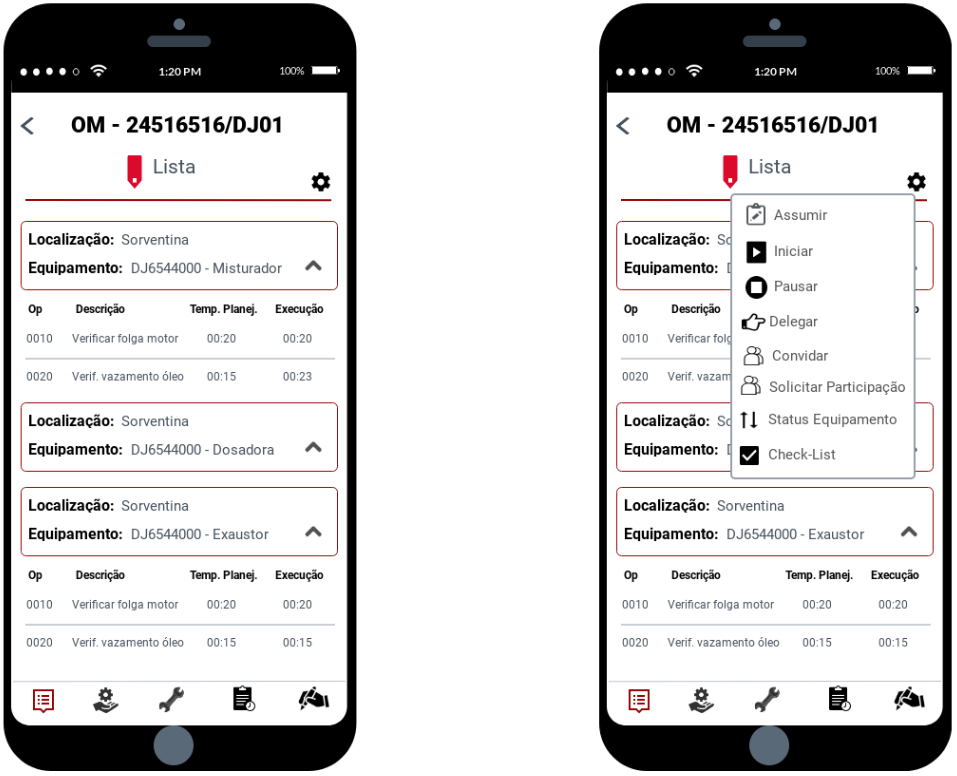
\includegraphics[scale=0.65]{./Figuras/mobile/lista.png}
	\end{center}
	\legend{Fonte: Próprio Autor, 2019}
\end{figure}

Na tela \ref{mobile_lista} será possível acompanhar o andamento de uma ordem de manutenção de lista, ver informações referente à ordem e executar ações nela, como alterar status, adicionar operações e realizar assinaturas.

\newpage
\subsection{Ordem de Manutenção: Rota}

\begin{figure}[htb]
	\caption{\label{mobile_rota}Ordem de Manutenção: Rota}
	\begin{center}
		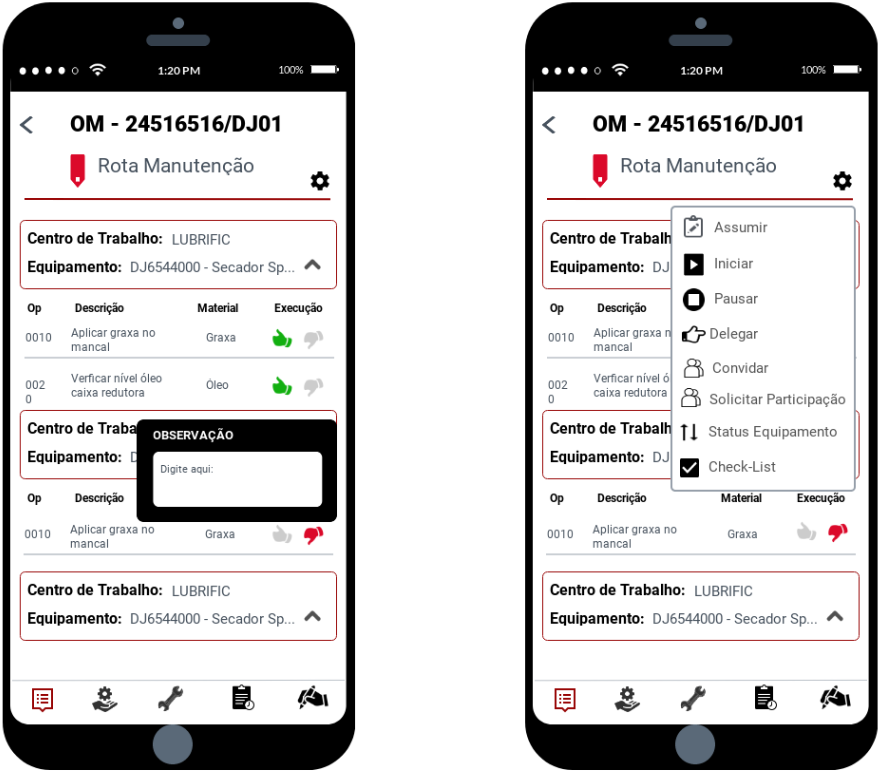
\includegraphics[scale=0.70]{./Figuras/mobile/rota.png}
	\end{center}
	\legend{Fonte: Próprio Autor, 2019}
\end{figure}

Na tela \ref{mobile_rota} será possível acompanhar o andamento de uma ordem de manutenção de rota, ver informações referente à ordem e executar ações nela, como alterar status, adicionar operações e realizar assinaturas.

\newpage
\subsection{Checklist de Segurança}

\begin{figure}[htb]
	\caption{\label{mobile_checklist}Checklist de Segurança}
	\begin{center}
		\includegraphics[scale=0.80]{./Figuras/mobile/checklist.png}
	\end{center}
	\legend{Fonte: Próprio Autor, 2019}
\end{figure}

Na tela \ref{mobile_checklist} o manutentor irá marcar a lista de segurança antes de iniciar a ordem de manutenção.

\newpage
\subsection{Problemas}

\begin{figure}[htb]
	\caption{\label{mobile_problema}Problemas}
	\begin{center}
		\includegraphics[scale=0.80]{./Figuras/mobile/problemas.png}
	\end{center}
	\legend{Fonte: Próprio Autor, 2019}
\end{figure}

Na tela \ref{mobile_problema} o manutentor irá verificar com maiores detalhes os problemas identificados no equipamento.

\newpage
\subsection{Componentes}

\begin{figure}[htb]
	\caption{\label{mobile_componentes}Componentes da Ordem de Manutenção}
	\begin{center}
		\includegraphics[scale=0.70]{./Figuras/mobile/componentes.png}
	\end{center}
	\legend{Fonte: Próprio Autor, 2019}
\end{figure}

Na tela \ref{mobile_componentes} é possível verificar todos os componentes utilizados na operação da ordem de manutenção.

\newpage
\subsection{Operações}

\begin{figure}[htb]
	\caption{\label{mobile_operacao}Operações da Ordem de Manutenção}
	\begin{center}
		\includegraphics[scale=0.70]{./Figuras/mobile/operacao.png}
	\end{center}
	\legend{Fonte: Próprio Autor, 2019}
\end{figure}

Na tela \ref{mobile_operacao} é possível verificar todas as operações pré cadastradas para a OM e cadastrar novas operações conforme necessidade para o andamento da OM.

\newpage
\subsection{Apontamentos}

\begin{figure}[htb]
	\caption{\label{mobile_apontamentos}Apontamentos da Ordem de Manutenção}
	\begin{center}
		\includegraphics[scale=0.80]{./Figuras/mobile/apontamentos.png}
	\end{center}
	\legend{Fonte: Próprio Autor, 2019}
\end{figure}

Na tela \ref{mobile_apontamentos} é possível realizar os apontamentos das horas trabalhadas na execução da ordem de manutenção.

\newpage
\subsection{Assinatura Digital}

\begin{figure}[htb]
	\caption{\label{mobile_assinaturas}Assinatura Digital}
	\begin{center}
		\includegraphics[scale=0.80]{./Figuras/mobile/assinaturas.png}
	\end{center}
	\legend{Fonte: Próprio Autor, 2019}
\end{figure}

Na tela \ref{mobile_assinaturas} é possível verificar e realizar as assinaturas.
\chapter{Planejamento do Sistema}

{\color{red} Dar uma introdução sobre esse capítulo, pois alterei a ordem deles}

\section{Cronograma do Projeto}


{\color{red} Vamos fazer um único cronograma do semestre ou fazer um por semestre?? Caso a segunda opção Padronizar a apresentação deles. Decidiremos em reunião }


Todo bom projeto deve ter um cronograma e um planejamento de ação, baseado nisso, foi elaborado dois cronogramas: um apresentando todo o conteúdo aprendido no semestre e outro montando plano de ação para implementação do projeto.

As figuras a seguir, são cronogramas que demonstram a trajetória do desenvolvimento do projeto. Divididos por semestre, os cronogramas listam as atividades aprendidas nas UCs, com todas as partes teóricas e práticas onde o objetivo principal é implementar todo conhecimento adquirido em prol de um projeto único: A unificação de todas as UCs do curso de Sistemas para Internet.

\begin{figure}[htb]
	\caption{\label{cron-3-semestre}Cronograma de Aprendizagem: Terceiro Semestre}
	\begin{center}
		\includegraphics[scale=0.90]{./Figuras/cronograma-3-semestre.png}
	\end{center}
\end{figure}


\begin{figure}[htb]
	\caption{\label{cron-4-semestre}Cronograma de Aprendizagem: Quarto Semestre}
	\begin{center}
		\includegraphics[scale=0.90]{./Figuras/cronograma-4-semestre.png}
	\end{center}
\end{figure}


\begin{figure}[htb]
	\caption{\label{cron-4-semestre}Cronograma de Aprendizagem: Quinto Semestre}
	\begin{center}
		\includegraphics[scale=0.70]{./Figuras/cronograma-5-semestre.png}
	\end{center}
\end{figure}


{\section{Análise de riscos}
	
	A análise de riscos tem como objetivo identificar os possíveis problemas durante e após o desenvolvimento do projeto a fim de elaborar um plano de ação para solucionar rapidamente o problema de fato \cite{schmitzanalise}.
	
	Segundo \cite{de2003engenharia}, um grande volume de dados publicados aponta para os riscos que correm os projetos de software executados sem a utilização de processos adequados. Um levantamento publicado, a partir de
	uma base de dados de 4.000 projetos, constatou a ocorrência frequente dos seguintes
	problemas: 
	
	\begin{itemize}
		
		\item 70\% dos projetos de grandes aplicativos sofre de instabilidade dos requisitos. Os requisitos crescem tipicamente cerca de 1\% ao mês, atingindo níveis de mais de 25\% de inchaço ao final
		do projeto.
		
		\item Pelo menos 50\% dos projetos são executados com níveis de produtividade abaixo do normal.
		
		\item Pelo menos 25\% do software de prateleira e 50\% dos produtos feitos por encomenda apresentam níveis de defeitos superiores ao razoável. 
		
		\item Produtos feitos sob pressão de prazos podem quadruplicar o número de defeitos.
		
		\item Pelo menos 50\% dos grandes projetos de software estouram seu orçamento e seu prazo. 
		
	\end{itemize}
	
	
	Sendo assim, foi identificado os fatores de risco, no qual o projeto em questão possa estar exposto. Nela, faz-se uma análise do impacto e probabilidade de fatores prejudiciais ao projeto, conforme tabela \ref{tebela_risco} abaixo.
	
	\begin{table}[]
		\caption{\label{tebela_risco} Tabela de Riscos Agil.it}
		\begin{tabular}{l|l|l}
			\hline
			\rowcolor[HTML]{EFEFEF} 
			\textbf{Riscos}                     & \textbf{Probabilidade} & \textbf{Impacto} \\ \hline
			\rowcolor[HTML]{DD7346} 
			Mudança de escopo                   & 90\%                   & 2                \\ \hline
			\rowcolor[HTML]{DD7346} 
			Entrega no prazo                    & 70\%                   & 3                \\ \hline
			\rowcolor[HTML]{DD7346} 
			Integração com SAP                  & 70\%                   & 2                \\ \hline
			\rowcolor[HTML]{FFFE65} 
			Implantação na empresa              & 60\%                   & 2                \\ \hline
			\rowcolor[HTML]{FFFE65} 
			Conexão com o banco de dados        & 60\%                   & 3                \\ \hline
			\rowcolor[HTML]{FFFE65} 
			Aceitação da usabilidade do sistema & 50\%                   & 2                \\ \hline
			\rowcolor[HTML]{FFFE65} 
			Usuários inexperientes              & 40\%                   & 2                \\ \hline
			\rowcolor[HTML]{9AFF99} 
			Mudanças na tecnologia              & 20\%                   & 3                \\ \hline
			\rowcolor[HTML]{9AFF99} 
			Segurança dos dados                 & 15\%                   & 2                \\ \hline
			\rowcolor[HTML]{9AFF99} 
			Conexão com a rede                  & 10\%                   & 2                \\ \hline
			\rowcolor[HTML]{9AFF99} 
			Falta de profissionais              & 5\%                    & 3                \\ \hline
		\end{tabular}
		\caption{Fonte: os autores (2020)}
	\end{table}
	
	
	{\color{red} Melhorar essa explicação e dar uma introduzida no sentido de utilização das cores também, por mais obvia que seja}
	
	Na tabela \ref{tebela_risco} estão mapeados os principais riscos identificados para o projeto Agil.It. Nela, a probabilidade indica a chance do risco ocorrer e o impacto é uma escala de um a três (1-3) do quanto o risco pode afetar a conclusão e entrega do projeto. A seguir será abordado o diagrama de causa e efeito.
	
	{\subsection{Diagrama de Causa e Efeito}
		
		{\color{red} Descrever Diagrama de Causa e Efeito com referencias}
		
		
		\begin{figure}[htb]
			\caption{\label{causaeefeito1}Diagrama de Causa e Efeito}
			\begin{center}
				\includegraphics[scale=0.55]{./Figuras/Diagrama causa e efeito.jpeg}
			\end{center}
			\legend{Fonte: os autores (2020)}
		\end{figure}
	}
	
	
	
	\section{PMBOK}
	
	{É uma metodologia de gerenciamento de projeto internacionalmente reconhecida, essas práticas podem auxiliar na resolução dos recursos humanos, capitais, tecnológicos e técnicos. Além disso, utilizando PMBOK é possível gerir melhor o andamento do projeto e de forma mais coordenada. Segundo \cite{PMG2018} o PMBOK tem conhecimentos já comprovados que são amplamente utilizados, assim como o conhecimento de práticas mais inovadoras e avançadas} Dentre as técnicas de planejamento, pode-se utilizar para estudos e desenvolvimento a EAP -  Estrutura Analítica de Projetos, descrita a seguir.
	
	\subsection{Estrutura Analítica do Projeto}
	
	
	
	{A Estrutura Analítica do Projeto (EAP) é a divisão estruturada de trabalho do projeto dividido em faixas gerenciadas cujo a sua totalidade significa em um entregável ao projeto final.
		
		Segundo \cite{PMI2018} o detalhamento da EAP deve chegar até o nível do pacote de trabalho, nível mais baixo na EAP, que é o ponto no qual o custo e o cronograma do trabalho podem ser estimados de forma confiável. Porém o nível de detalhamento desse pacote varia de acordo com a complexidade de cada projeto. \cite{kerzner2017} defende que a EAP deve ser composta por até três níveis pois se for detalhado com demaseio o custo com o gerenciamento serão também excessivos.}
	
	Para o projeto Agil-it foi decidido utilizar 6 faixas de entregáveis:
	
	\begin{subalineas}
		\item {Planejamento};
		\item {Análise};
		\item {Implementação Web};
		\item {Implementação Mobile};
		\item {Testes};
		\item {Implantação}.
	\end{subalineas}
	
	
	\begin{landscape}
		\begin{figure}[htb]
			\caption{\label{EAP}EAP AGIL.IT}
			\begin{center}
				\includegraphics[scale=0.38]{./Figuras/EAP.png}
			\end{center}
			\legend{Fonte: os autores (2020)}
		\end{figure}
	\end{landscape}
	
	A figura \ref{EAP} mostra a estrutura e o desenvolvimento que cada faixa requer no projeto. Ela não segue uma ordem cronológica, portanto não é necessário finalizar uma faixa para começar outra, muitas vezes elas são desenvolvidas em conjunto para uma melhor utilização do tempo de projeto.
	
	
	\subsection{Fluxo de Processos}
	% ---
	
	{O fluxo de processo é subdividido em cinco fases principais sobre o fluxo do projeto, iniciação sendo a primeira seguindo de planejamento, execução, monitoramento, controle e finalização. Para \cite{PMG2018} um projeto é desenvolvido a partir de uma idéia, em seguida parte para um plano e após isso é executado e concluído.}
	
	Para a definição dos processos, foi utilizado os seguintes recursos:
	
	\begin{subalineas}
		\item {Partes Interessadas};
		\item {Escopo};
		\item {Tempo};
		\item {Recursos Humanos};
		\item {Aquisições};
		\item {Qualidade};
		\item {Comunicações};
		\item {Riscos}.
	\end{subalineas}
	
	A figura abaixo contém todos os fluxos desenhados para o projeto.{\color{red}chamar pelo numero da figura não abaixo}
	{\color{red} Usar h para forçar a imagem ficar no local}
	
	\begin{figure}[h]
		\caption{\label{Fluxo-Processos}Fluxo e Processos AGIL.IT}
		\begin{center}
			\includegraphics[scale=0.24]{./Figuras/fluxo-processos.png}
		\end{center}
		\legend{Fonte: os autores (2020)}
	\end{figure}
	
	
	
	{\textbf{Iniciação} - Esta é a fase inicial do projeto, nela é determinado a necessidade do projeto, com seus objetivos e justificativas, então é realizado os documentos iniciais onde as melhores estratégias são identificadas e selecionadas.}
	
	{\textbf{Planejamento} - Fase onde deve ser detalhado minuciosamente tudo aquilo que será realizado no projeto, desde cronogramas, interdependências entre atividades, alocação dos recursos envolvidos, análise de custos etc. Esta parte é muito importante pois a execução do projeto será em cima destas atividades para que sejam executadas sem dificuldades e imprevistos.}
	
	{\textbf{Execução} - Nesta fase tudo é onde tudo que foi planejado anteriormente se torne realidade, tendo que ser executado e realizado conforme planejado, qualquer erro cometidas nas fases anteriores fica evidente durante essa fase. }
	
	{\textbf{Monitoramento e Controle} - Esta fase acontece paralelamente às demais fases do projeto, acompanhando e controlando aquilo que está sendo realizado no projeto como um todo, podendo propor ações corretivas e preventivas no menor espaço de tempo possível após a detecção de erros.}
	
	
	\section{Protótipo}
	
	{\color{red} Reduzir o numero de imagens dessa section}
	
	A prototipação é uma etapa de suma importância no desenvolvimento de projeto de software. Além de melhorar a produtividade da equipe, ela facilita o entendimento dos requisitos do sistema e permite a apresentação de de conceitos e funcionalidades da aplicação de modo simplificado.
	Nesse trabalho foi utilizado a prototipação visual cujo ênfase se aplica a estética e usabilidade. Nesse tipo de protótipo é possível identificar o layout e a identidade visual da aplicação. \cite{dextra2013prototipacao}
	
	{Protótipos podem ser gerados de acordo com as seguintes categorias \cite{coyette2004sketchixml}: protótipos em baixa fidelidade que focam na interação, em componentes de interface e na estrutura geral do sistema; protótipos em alta fidelidade que produzem uma imagem real do sistema; protótipos executáveis que produzem o código em uma linguagem de programação, focando em navegação, mas sem ainda levar em consideração as regras de negócio. Cada categoria serve para um propósito específico: protótipos em baixa fidelidade são úteis para demonstrar aos usuários quais atividades o sistema atende e as possibilidades de navegação no sistema, assim como para proporcionar uma visão geral do sistema. Protótipos em alta fidelidade são úteis para demonstrar padrões e guias de estilo. Protótipos executáveis são úteis para demonstrar navegação e testar o uso da interface \cite{rosemberg2008prototipaccao}.Seguindo as definições, o projeto desenvolvido utiliza os protótipos de baixa fidelidade}
	
	\section{Aplicação WEB}
	A aplicação web tem como foco o gerenciamento de toda a aplicação envolvendo consultas e cadastros gerais do sistema.
	Apesar desse foco acentuado à gestão, é possível desempenhar todos os papeis dentro da aplicação web.
	
	
	\subsection{Login}
	
	\begin{figure}[htb]
		\caption{\label{web_login}Tela de Login do Agil.It}
		\begin{center}
			\includegraphics[scale=0.70]{./Figuras/web/login.png}
		\end{center}
		\legend{Fonte: os autores (2020)}
	\end{figure}
	
	A tela \ref{web_login} será a página responsável por autenticar os usuários e garantir a segurança do sistema.
	
	
	\subsection{Cadastro de Ordem de Manutenção}
	
	\begin{figure}[htb]
		\caption{\label{web_cad-om}Cadastro de Ordem de Manutenção}
		\begin{center}
			\includegraphics[scale=0.65]{./Figuras/web/cad-om.png}
		\end{center}
		\legend{Fonte: os autores (2020)}
	\end{figure}
	
	Na tela \ref{web_cad-om} é cadastrada e atualizada ordens de manutenção. Ela terá acesso às operações, componentes e assinaturas.
	
	
	\subsection{Monitor de Ordem de Manutenção: Cards}
	
	\begin{figure}[htb]
		\caption{\label{web_monitor-om-card}Monitor de Ordem de Manutenção: Cards}
		\begin{center}
			\includegraphics[scale=0.45]{./Figuras/web/monitor-om-card.png}
		\end{center}
		\legend{Fonte: os autores (2020)}
	\end{figure}
	
	A tela \ref{web_monitor-om-card} permite a consulta rápida e dinâmica das ordens de manutenção. Nela você pode aplicar os filtros de acordo com as \newline necessidades e será listada em forma de cartões, eles darão acesso à uma tela de detalhamento de ordem de manutenção.
	
	\newpage
	\subsection{Monitor de Ordem de Manutenção: Listas}
	
	\begin{figure}[htb]
		\caption{\label{web_monitor-om-lista}Monitor de Ordem de Manutenção: Listas}
		\begin{center}
			\includegraphics[scale=0.45]{./Figuras/web/monitor-om-lista.png}
		\end{center}
		\legend{Fonte: os autores (2020)}
	\end{figure}
	
	A tela \ref{web_monitor-om-lista} permite a consulta rápida e dinâmica das ordens de manutenção. Nela você pode aplicar os filtros de acordo com as \newline necessidades e será listada em forma de listas, eles darão acesso à uma tela de detalhamento de ordem de manutenção.
	
	\newpage
	\subsection{Ordem de Manutenção}
	
	\begin{figure}[htb]
		\caption{\label{web_om-capa}Ordem de Manutenção}
		\begin{center}
			\includegraphics[scale=0.40]{./Figuras/web/om-capa.png}
		\end{center}
		\legend{Fonte: os autores (2020)}
	\end{figure}
	
	Na tela \ref{web_om-capa} será possível acompanhar o andamento de uma ordem de manutenção de lista, ver informações referente à ordem e executar ações nela, como alterar status, adicionar operações e realizar assinaturas.
	
	\newpage
	\subsection{Checklist de Segurança}
	
	\begin{figure}[htb]
		\caption{\label{web_check-list}Checklist de Segurança}
		\begin{center}
			\includegraphics[scale=0.40]{./Figuras/web/check-list.png}
		\end{center}
		\legend{Fonte: os autores (2020)}
	\end{figure}
	
	Na tela \ref{web_check-list} o manutentor irá marcar a lista de segurança antes de iniciar a ordem de manutenção.
	
	\newpage
	\subsection{Operações da Ordem de Manutenção}
	
	\begin{figure}[htb]
		\caption{\label{web_om-operacoes}Operações da Ordem de Manutenção}
		\begin{center}
			\includegraphics[scale=0.40]{./Figuras/web/om-operacoes.png}
		\end{center}
		\legend{Fonte: os autores (2020)}
	\end{figure}
	
	Na tela \ref{web_om-operacoes} é possível verificar todas as operações pré cadastradas para a OM e cadastrar novas operações conforme necessidade para o andamento da OM.
	
	\newpage
	\subsection{Ordem de Manutenção: Lista}
	
	\begin{figure}[htb]
		\caption{\label{web_om-lista}Ordem de Manutenção: Lista}
		\begin{center}
			\includegraphics[scale=0.40]{./Figuras/web/om-lista.png}
		\end{center}
		\legend{Fonte: os autores (2020)}
	\end{figure}
	
	Na tela \ref{web_om-lista} será possível acompanhar o andamento de uma ordem de manutenção de lista, ver informações referente à ordem e executar ações nela, como alterar status, adicionar operações e realizar assinaturas.
	
	\newpage
	\subsection{Equipamentos da Ordem de Manutenção: Lista}
	
	\begin{figure}[htb]
		\caption{\label{web_om-lista-equipamentos}Equipamentos da Ordem de Manutenção: Lista}
		\begin{center}
			\includegraphics[scale=0.40]{./Figuras/web/om-lista-equipamentos.png}
		\end{center}
		\legend{Fonte: os autores (2020)}
	\end{figure}
	
	Na tela \ref{web_om-lista-equipamentos} será possível acompanhar os equipamentos que terão de ser inspecionados pelo manutentor e o mesmo marcar se executou ou não.
	
	\newpage
	\subsection{Ordem de Manutenção: Rota}
	
	\begin{figure}[htb]
		\caption{\label{web_om-rota}Ordem de Manutenção: Rota}
		\begin{center}
			\includegraphics[scale=0.40]{./Figuras/web/om-rota.png}
		\end{center}
		\legend{Fonte: os autores (2020)}
	\end{figure}
	
	Na tela \ref{web_om-rota} será possível acompanhar o andamento de uma ordem de manutenção de lista, ver informações referente à ordem e executar ações nela, como alterar status, adicionar operações e realizar assinaturas.
	
	\newpage
	\subsection{Convidar ou Delegar Ordem de Manutenção}
	
	\begin{figure}[htb]
		\caption{\label{web_om-convidar-delegar}Convidar ou Delegar Ordem de Manutenção}
		\begin{center}
			\includegraphics[scale=0.40]{./Figuras/web/om-convidar-delegar.png}
		\end{center}
		\legend{Fonte: os autores (2020)}
	\end{figure}
	
	Na tela \ref{web_om-convidar-delegar} será possível convidar técnicos para se juntarem a ordem de manutenção ou delegar a ordem de manutenção a outro manutentor. Ação só permitida àqueles que são responsáveis pela ordem de manutenção, ou seja, os que assumiram ela.
	
	\newpage
	\subsection{Apontamentos}
	
	\begin{figure}[htb]
		\caption{\label{web_om-apontamentos}Apontamentos da Ordem de Manutenção}
		\begin{center}
			\includegraphics[scale=0.40]{./Figuras/web/om-apontamentos.png}
		\end{center}
		\legend{Fonte: os autores (2020)}
	\end{figure}
	
	Na tela \ref{web_om-apontamentos} será possível visualizar todos os apontamentos que existem em uma ordem, atualizá-las, excluí-las ou adicionar novos apontamentos.
	
	\newpage
	\subsection{Adicionar Apontamentos}
	
	\begin{figure}[htb]
		\caption{\label{web_om-add-apontamento}Adicionar Apontamentos na Ordem de Manutenção}
		\begin{center}
			\includegraphics[scale=0.40]{./Figuras/web/om-add-apontamento.png}
		\end{center}
		\legend{Fonte: os autores (2020)}
	\end{figure}
	
	Na tela \ref{web_om-add-apontamento} será possível adicionar novos apontamentos a ordem de manutenção.
	
	\newpage
	\subsection{Motivo da Exclusão do Apontamento da Ordem de Manutenção}
	
	\begin{figure}[htb]
		\caption{\label{web_om-excluir-apontamento-motivo}Motivo da Exclusão do Apontamento da Ordem de Manutenção}
		\begin{center}
			\includegraphics[scale=0.40]{./Figuras/web/om-excluir-apontamento-motivo.png}
		\end{center}
		\legend{Fonte: os autores (2020)}
	\end{figure}
	
	Na tela \ref{web_om-excluir-apontamento-motivo} o operador terá de informar o motivo pela exclusão do apontamento da ordem de manutenção.
	
	\newpage
	\subsection{Assinatura Digital}
	
	\begin{figure}[htb]
		\caption{\label{web_om-assinatura}Assinatura Digital}
		\begin{center}
			\includegraphics[scale=0.40]{./Figuras/web/om-assinatura.png}
		\end{center}
		\legend{Fonte: os autores (2020)}
	\end{figure}
	
	Na tela \ref{web_om-assinatura} será possível assinar a ordem digitalmente. Para tanto, será cobrado as credenciais do operador.
	
	\newpage
	\section{Aplicação Mobile}
	A aplicação Mobile é um ponto estratégico do produto, pois sua mobilidade permite com que os técnicos possam atuar na manutenção e realizar anotações e apontamentos no sistema através de um smartphone ou tablet.
	
	\subsection{Login}
	
	\begin{figure}[htb]
		\caption{\label{mobile_login}Login}
		\begin{center}
			\includegraphics[scale=0.80]{./Figuras/mobile/login.png}
		\end{center}
		\legend{Fonte: os autores (2020)}
	\end{figure}
	
	A tela \ref{mobile_login} será a página responsável por autenticar o usuário e garantir a segurança do sistema.
	
	\newpage
	\subsection{Menu}
	
	\begin{figure}[htb]
		\caption{\label{mobile_menu}Menu}
		\begin{center}
			\includegraphics[scale=0.80]{./Figuras/mobile/menu.png}
		\end{center}
		\legend{Fonte: os autores (2020)}
	\end{figure}
	
	A figura \ref{mobile_menu} demonstra o menu lateral do aplicativo, identificando o usuário autenticado e um menu de acesso rápido às principais telas do sistema.
	
	\newpage
	\subsection{Monitor}
	
	\begin{figure}[htb]
		\caption{\label{mobile_monitor}Monitor}
		\begin{center}
			\includegraphics[scale=0.75]{./Figuras/mobile/monitor.png}
		\end{center}
		\legend{Fonte: os autores (2020)}
	\end{figure}
	
	Na figura \ref{mobile_monitor} é possível verificar o monitor do manutentor. Nesse monitor, o manutentor consegue rapidamente visualizar as OMs pendentes e seus respectivos status através das bandeiras indicadas no card. As  vermelhas indicam que a OM tem uma prioridade emergente, as amarelas têm prioridade alta, as azuis têm prioridade média e as verdes possuem uma prioridade baixa.
	
	\newpage
	\subsection{Central de Notificações}
	
	\begin{figure}[htb]
		\caption{\label{mobile_notificacao}Notificações}
		\begin{center}
			\includegraphics[scale=0.80]{./Figuras/mobile/notificacao.png}
		\end{center}
		\legend{Fonte: os autores (2020)}
	\end{figure}
	
	Na tela \ref{mobile_notificacao} é possível verificar notificações do usuário autenticado no sistema.
	
	\newpage
	\subsection{Ordem de Manutenção}
	
	\begin{figure}[htb]
		\caption{\label{mobile_om}Ordem de Manutenção}
		\begin{center}
			\includegraphics[scale=0.70]{./Figuras/mobile/om.png}
		\end{center}
		\legend{Fonte: os autores (2020)}
	\end{figure}
	
	Na tela \ref{mobile_om} será possível acompanhar o andamento de uma ordem de manutenção preventiva e corretiva, ver informações referente à ordem e executar ações nela, como alterar status, adicionar operações e realizar assinaturas.
	
	\newpage
	\subsection{Ordem de Manutenção: Lista}
	
	\begin{figure}[htb]
		\caption{\label{mobile_lista}Ordem de Manutenção: Lista}
		\begin{center}
			\includegraphics[scale=0.65]{./Figuras/mobile/lista.png}
		\end{center}
		\legend{Fonte: os autores (2020)}
	\end{figure}
	
	Na tela \ref{mobile_lista} será possível acompanhar o andamento de uma ordem de manutenção de lista, ver informações referente à ordem e executar ações nela, como alterar status, adicionar operações e realizar assinaturas.
	
	\newpage
	\subsection{Ordem de Manutenção: Rota}
	
	\begin{figure}[htb]
		\caption{\label{mobile_rota}Ordem de Manutenção: Rota}
		\begin{center}
			\includegraphics[scale=0.70]{./Figuras/mobile/rota.png}
		\end{center}
		\legend{Fonte: os autores (2020)}
	\end{figure}
	
	Na tela \ref{mobile_rota} será possível acompanhar o andamento de uma ordem de manutenção de rota, ver informações referente à ordem e executar ações nela, como alterar status, adicionar operações e realizar assinaturas.
	
	\newpage
	\subsection{Checklist de Segurança}
	
	\begin{figure}[htb]
		\caption{\label{mobile_checklist}Checklist de Segurança}
		\begin{center}
			\includegraphics[scale=0.80]{./Figuras/mobile/checklist.png}
		\end{center}
		\legend{Fonte: os autores (2020)}
	\end{figure}
	
	Na tela \ref{mobile_checklist} o manutentor irá marcar a lista de segurança antes de iniciar a ordem de manutenção.
	
	\newpage
	\subsection{Problemas}
	
	\begin{figure}[htb]
		\caption{\label{mobile_problema}Problemas}
		\begin{center}
			\includegraphics[scale=0.80]{./Figuras/mobile/problemas.png}
		\end{center}
		\legend{Fonte: os autores (2020)}
	\end{figure}
	
	Na tela \ref{mobile_problema} o manutentor irá verificar com maiores detalhes os problemas identificados no equipamento.
	
	\newpage
	\subsection{Componentes}
	
	\begin{figure}[htb]
		\caption{\label{mobile_componentes}Componentes da Ordem de Manutenção}
		\begin{center}
			\includegraphics[scale=0.70]{./Figuras/mobile/componentes.png}
		\end{center}
		\legend{Fonte: os autores (2020)}
	\end{figure}
	
	Na tela \ref{mobile_componentes} é possível verificar todos os componentes utilizados na operação da ordem de manutenção.
	
	\newpage
	\subsection{Operações}
	
	\begin{figure}[htb]
		\caption{\label{mobile_operacao}Operações da Ordem de Manutenção}
		\begin{center}
			\includegraphics[scale=0.70]{./Figuras/mobile/operacao.png}
		\end{center}
		\legend{Fonte: os autores (2020)}
	\end{figure}
	
	Na tela \ref{mobile_operacao} é possível verificar todas as operações pré cadastradas para a OM e cadastrar novas operações conforme necessidade para o andamento da OM.
	
	\newpage
	\subsection{Apontamentos}
	
	\begin{figure}[htb]
		\caption{\label{mobile_apontamentos}Apontamentos da Ordem de Manutenção}
		\begin{center}
			\includegraphics[scale=0.80]{./Figuras/mobile/apontamentos.png}
		\end{center}
		\legend{Fonte: os autores (2020)}
	\end{figure}
	
	Na tela \ref{mobile_apontamentos} é possível realizar os apontamentos das horas trabalhadas na execução da ordem de manutenção.
	
	\newpage
	\subsection{Assinatura Digital}
	
	\begin{figure}[htb]
		\caption{\label{mobile_assinaturas}Assinatura Digital}
		\begin{center}
			\includegraphics[scale=0.80]{./Figuras/mobile/assinaturas.png}
		\end{center}
		\legend{Fonte: os autores (2020)}
	\end{figure}
	
	Na tela \ref{mobile_assinaturas} é possível verificar e realizar as assinaturas.


\chapter{Considerações e Trabalhos Futuros}

{Com a análise de requisitos executada no semeste anterior, conseguimos dar continuidade com o desenvolvimento das aplicações com base neles propostos. Também será melhorada a parte documental e adicionado funcionalidades específicas necessárias para a entrega final do projeto. Desta maneira, será de suma importância a participação direta dos envolvidos para o desenvolvimento competente e satisfatório para a execução e implantação do Projeto Integrador. }



% ---
% Finaliza a parte no bookmark do PDF, para que se inicie o bookmark na raiz
% ---
\bookmarksetup{startatroot}% 
% ---

% ----------------------------------------------------------
% ELEMENTOS PÓS-TEXTUAIS
% ----------------------------------------------------------
\postextual


% ----------------------------------------------------------
 %Referências bibliográficas
% ----------------------------------------------------------
\bibliography{references}

% ----------------------------------------------------------
% Glossário
% ----------------------------------------------------------
%
% Consulte o manual da classe abntex2 para orientações sobre o glossário.
%
%\glossary

% ----------------------------------------------------------
% Apêndices
% ----------------------------------------------------------
%\begin{apendicesenv}

% Imprime uma página indicando o início dos apêndices
%\partapendices

%% ----------------------------------------------------------
\chapter{Quisque libero justo}
% ----------------------------------------------------------

\lipsum[50]

% ----------------------------------------------------------
\chapter{Nullam elementum urna vel imperdiet sodales elit ipsum pharetra ligula
ac pretium ante justo a nulla curabitur tristique arcu eu metus}
% ----------------------------------------------------------
\lipsum[55-57]


%\end{apendicesenv}

% ----------------------------------------------------------
% Anexos

% ----------------------------------------------------------
%\begin{anexosenv}

% Imprime uma página indicando o início dos anexos
%\partanexos

%\include{anexo}

%\end{anexosenv}

%---------------------------------------------------------------------
% INDICE REMISSIVO
%---------------------------------------------------------------------

%\printindex

\end{document}
% FIM